\documentclass[12pt]{exam}
\newcommand{\Solutions}{1} 
\newcommand{\SetNumber}{0} % can set this variable to zero here it gets updated automatically later



\begin{document}

    \foreach \i in {0,...,9} {
    \newcommand{\Version}{\i}

    % TEST SPECIFIC INFORMATION
    \ifnum \Version=0 \newcommand{\TestName}{Year 1 MATH 1554 Exam 2 Sample A} \fi % already in Canvas
    \ifnum \Version=1 \newcommand{\TestName}{Year 1 MATH 1554 Exam 2 Sample B} \fi
    \ifnum \Version=2 \newcommand{\TestName}{Year 1 MATH 1554 Exam 2 Sample C} \fi
    \ifnum \Version=3 \newcommand{\TestName}{Year 1 MATH 1554 Exam 2 Sample D} \fi
    \ifnum \Version=4 \newcommand{\TestName}{Year 1 MATH 1554 Exam 2 Sample E} \fi
    
    \ifnum \Version=6 \newcommand{\TestName}{Year 1 MATH 1554 Exam 2 Version A1} \fi 
    \ifnum \Version=7 \newcommand{\TestName}{Year 1 MATH 1554 Exam 2 Version B} \fi 
    \ifnum \Version=8 \newcommand{\TestName}{Year 1 MATH 1554 Exam 2 Version C} \fi 
    \ifnum \Version=5 \newcommand{\TestName}{Year 1 MATH 1554 Exam 2 Version D} \fi % revised fall 2022 exam 
    \ifnum \Version=20 \newcommand{\TestName}{Year 1 MATH 1554 Exam 2 Version A2} \fi 
    
    
    % UPDATE SET NUMBER FOR ADDITIONAL RANDOMIZATION
    \ifnum \Version=0 \renewcommand{\SetNumber}{1} \fi
    \ifnum \Version=1 \renewcommand{\SetNumber}{1} \fi
    \ifnum \Version=2 \renewcommand{\SetNumber}{2} \fi
    \ifnum \Version=3 \renewcommand{\SetNumber}{1} \fi
    \ifnum \Version=4 \renewcommand{\SetNumber}{2} \fi
    \ifnum \Version=5 \renewcommand{\SetNumber}{1} \fi
    \ifnum \Version=6 \renewcommand{\SetNumber}{2} \fi
    \ifnum \Version=7 \renewcommand{\SetNumber}{1} \fi
    \ifnum \Version=8 \renewcommand{\SetNumber}{2} \fi
    \ifnum \Version=9 \renewcommand{\SetNumber}{1} \fi
    \ifnum \Version=20 \renewcommand{\SetNumber}{2} \fi
    
    \newpage % ensures each exam is on its own page

    % MAKE VERSION A2 = C
    \ifnum \Version = 20
        \renewcommand{\Version}{8}
    \fi

    
    % TITLE
    \begin{center}
    \ifnum \Solutions=1 {\Large {\color{DarkBlue}\textit{Solutions}}\\[6pt]}\fi
    {\Large \TestName}
    \end{center}
    
    \textit{Work done on scratch paper will not be graded. You do not need to show your work on page 1. }
    
    \begin{questions}
    
    \ifnum \SetNumber=1    
        \question[0.5] \ID
        \question[9] Indicate \textbf{true} if the statement is true, otherwise, indicate \textbf{false}.

\vspace{-0.8cm}
\setlength{\extrarowheight}{0.20cm}
\begin{center}
\hspace{-.9cm}\begin{tabular}[H]{ p{.15cm} p{14.2cm} p{.6cm} p{.6cm} }
       & & true &  false  \\[2pt] \hline 
    
    % DETERMINANTS
    a) &  
    \ifnum \Version=0      
        If $\det(A) =0$, then zero is a root of the characteristic polynomial of $A$. 
        \ifnum \Solutions=1 {\color{DarkBlue} \textit{Solution: true, because if $\det A = 0$, then the matrix will be singular, and singular matrices have a zero eigenvalue.}  } \fi
    \fi            
    \ifnum \Version=1         
        If $A$ is $n\times n$, and $A$ does not have $n$ pivots, then $\text{det}(A) = 0$.
        \ifnum \Solutions=1 {\color{DarkBlue} \textit{Solution: } true, because the determinant of a singular matrix is zero. } \fi
    \fi
    \ifnum \Version=2      
        If $A$ is square and row equivalent to an identity matrix, then det$(A) \ne 0$.
        \ifnum \Solutions=1 {\color{DarkBlue} 
        \textit{Solution:} true, because the matrix will be invertible, and the determinant of an invertible matrix is non-zero.}   \fi
    \fi    
    \ifnum \Version=3  
        If $A$ is $n\times n$, and there exists a $\vec b \in \mathbb R^n$ such that $A\vec x = \vec b$ is inconsistent, then $\text{det}(A) = 0$.    
        \ifnum \Solutions=1 {\color{DarkBlue} \textit{Solution: true, because the matrix will be singular, and the determinant of an singular matrix is zero.}  } \fi
    \fi    
    \ifnum \Version=4    
        Swapping the rows of $A$ does not change the value of $\text{det}(A)$.
        \ifnum \Solutions=1 {\color{DarkBlue} \textit{False. This is a property of determinants. Swapping a row changes the sign of the determinant.}  } \fi
    \fi   
    \ifnum \Version=5    
        Swapping the rows of $A$ does not change the value of $\text{det}(A)$.
        \ifnum \Solutions=1 {\color{DarkBlue} \textit{Solution: false, a property of determinants is that swapping rows changes the sign of the determinant. }  } \fi
    \fi    
    \ifnum \Version=6
        If $A$ is a $n\times n$, and  $\text{det}(A) = 3$, then  $Ax=b$ has a solution for all $b\in \mathbb R^n$. 
        \ifnum \Solutions=1 {\color{DarkBlue} \textit{Solution: } True. The determinant is non-zero, so matrix is invertible, and $x= A^{-1}b$ is the solution. } \fi
    \fi    
    \ifnum \Version=7
        If $E$ is a $2\times2$ elementary matrix, then $\text{det}(E) = 1$.
        \ifnum \Solutions=1 {\color{DarkBlue} \textit{Solution: false. An elementary matrix is any square matrix that is obtained by applying one row operation to the identity. For example \setlength{\extrarowheight}{0.0cm} $E = \begin{pmatrix} 2&0\\0&1 \end{pmatrix}$ is an elementary matrix, and $\det A \ne 0$. }  } \fi
    \fi    
    \ifnum \Version=8
         If $A$ is a $n\times n$, and  $\text{det}(A) = 3$, then $3$ is an eigenvalue of $A$. 
        \ifnum \Solutions=1 {\color{DarkBlue} \textit{Solution: } False. The number 3 is an eigenvalue when $\text{det}(A - 3I) = 0$, not when $\det A = 3$. } \fi
    \fi   
    \ifnum \Version=9
        If $E$ is n $n\times n$ elementary matrix, then $\text{det}(E) \ne 0$.
        \ifnum \Solutions=1 {\color{DarkBlue} \textit{Solution: True. An elementary matrix is any square matrix that is obtained by applying one row operation to the identity. So all elementary matrices are row equivalent to the identity, so they must also be invertible. Invertible matrices have non-zero determinants. }  } \fi
    \fi        
    & $\bigcirc$  & $\bigcirc$ \\
    
    % STOCHASTIC
    b) & 
    \ifnum \Version=0      
    The set of all probability vectors in $\mathbb R^n$ forms a subspace of $\mathbb R^n$.
        \ifnum \Solutions=1 {\color{DarkBlue} \textit{Solution: } false, because if $v$ is a probability vector, then $kv$ is not a probability vector for every $k$. } \fi
    \fi          
    \ifnum \Version=1         
        If $A$ is an $n\times n$ stochastic matrix and $\vec p$ is a column of $A$, then $\vec p$ is a probability vector. 
        \ifnum \Solutions=1 {\color{DarkBlue} \textit{Solution: } true, because the columns of a stochastic matrix are probability vectors (by definition).  } \fi
    \fi
    \ifnum \Version=2   
        The steady state of a stochastic matrix is unique. \ifnum \Solutions=1 {\color{DarkBlue} false, a counterexample would be the chain $x_{k+1} = Px_k$ with $P = I_n$.   } \fi
    \fi    
    \ifnum \Version=3  
        A steady-state vector of a regular stochastic matrix $P$ is unique. 
        \ifnum \Solutions=1 {\color{DarkBlue} \textit{Solution: } true, this is one of the theorems we covered in lecture and is given in the textbook. Regularity means starting from any state of the Markov Chain, one will visit every other state.} \fi
    \fi    
    \ifnum \Version=4      
        Any stochastic matrix with a zero entry cannot be regular.
        \ifnum \Solutions=1 {\color{DarkBlue} \textit{Solution: } false, if $P$ is a $3\times 3$ stochastic matrix with only one zero entry, then $P$ will have the property that every entry of $P^2$ is positive.} \fi
    \fi   
    \ifnum \Version=5      
        If $q$ is a steady-state vector for stochastic matrix $P$, then the Markov Chain $x_{k+1} = Px_k$ converges to $q$ as $k \to \infty$. 
        \ifnum \Solutions=1 {\color{DarkBlue} \textit{Solution: } false, we are only guaranteed that the chain converges to its steady state when it is regular.} \fi
    \fi    
    \ifnum \Version=6
         A steady-state vector of a stochastic matrix $P$ is unique. 
        \ifnum \Solutions=1 {\color{DarkBlue} \textit{Solution: } False. Think of a Chain where state A only goes to A, and B only goes to B. Regularity is required for uniqueness of the Markov state.  Regularity means starting from any state of the Markov Chain, one will visit every other state.} \fi
    \fi    
    \ifnum \Version=7
        $1$ is always an eigenvalue for any stochastic matrix $P$. 
        \ifnum \Solutions=1 {\color{DarkBlue} \textit{Solution: } True. A steady state always exists for any stochastic matrix, and the steady-state is an eigenvector associated with eigenvalue $1$.} \fi
    \fi    
    \ifnum \Version=8
        A steady state vector of a regular stochastic matrix only has positive entries.  
        \ifnum \Solutions=1 {\color{DarkBlue} \textit{Solution: } True. Because the steady state is defined as a probability vector, and probability vectors have entries that are between 0 and 1. Also because regular means that every state can visit every other state, so every entry of the steady state vector must be positive. } \fi
    \fi        
    & $\bigcirc$  & $\bigcirc$ \\ 




    % EIG 1 EASY
    c) & 
    \ifnum \Version=0      
        Row operations on a matrix do not change its eigenvalues. 
        \ifnum \Solutions=1 {\color{DarkBlue} \textit{Solution: false, row operations can change the eigenvalues of a matrix. Change the rows on the $2\times 2$ Identity, for instance.}  } \fi
    \fi          
    \ifnum \Version = 1
        If $A$ is $n\times n$ and upper triangular then the eigenvalues of $A$ are non-zero. 
        \ifnum \Solutions=1 {\color{DarkBlue} \textit{Solution: false, because for example the matrix \setlength{\extrarowheight}{0.00cm} $\begin{pmatrix} -1&0\\0&0\end{pmatrix}$ is upper triangular and has eigenvalues $-1$ and $0$.}  } \fi
    \fi
    \ifnum \Version=2      
        A $2\times 2$ matrix $A$ whose rank is $1$ must have an eigenvalue that is equal to zero. 
        \ifnum \Solutions=1 {\color{DarkBlue} \textit{Solution: } true, because the matrix must be singular if its rank is only 1, and singular matrices have at least one eigenvalue that is equal to zero. } \fi
    \fi    
    \ifnum \Version=3  
        If $\lambda=0$ is an eigenvalue of $A$, then the matrix $A$ is non-singular.    
        \ifnum \Solutions=1 {\color{DarkBlue} \textit{Solution: false, if an eigenvalue is zero the matrix must be non-invertible.}  } \fi
    \fi    
    \ifnum \Version=4      
        An eigenspace is a subspace spanned by a single eigenvector.
        \ifnum \Solutions=1 {\color{DarkBlue} \textit{Solution: false because an eigenspace is a subspace, but an eigenspace can be spanned by two eigenvectors. Take for example the matrix $A = \begin{pmatrix} 1&0&0\\0&2&0\\0&0&2\end{pmatrix}$ The eigenspace for eigenvalue $\lambda = 2$ is two dimensional. }  } \fi
    \fi   
    \ifnum \Version=5      
        An eigenvalue of a matrix could be associated with two linearly independent eigenvectors. 
        \ifnum \Solutions=1 {\color{DarkBlue} \setlength{\extrarowheight}{0.0cm} \textit{Solution: true, for example $A = \begin{pmatrix} 2&0\\0 & 2 \end{pmatrix}$ has eigenvalue $\lambda = 2$, and the eigenvectors $\begin{pmatrix}1\\0 \end{pmatrix}$ and $\begin{pmatrix}0\\1 \end{pmatrix}$ are associated with $\lambda = 2$.  }  } \fi
    \fi    
    \ifnum \Version=6
         An eigenspace of a square matrix $A$ has a basis that consists of eigenvectors. 
        \ifnum \Solutions=1 {\color{DarkBlue} \textit{Solution: } True. Every non-zero vector in an eigenspace is an eigenvector. So any basis consists only of eigenvectors. } \fi
    \fi    
    \ifnum \Version=7
        The dimension of an eigenspace of a square matrix $A $ is one. 
        \ifnum \Solutions=1 {\color{DarkBlue} \textit{Solution: } False. The eigenspace of the $n\times n$ identity matrix is $\mathbb R^n$.   } \fi
    \fi    
    \ifnum \Version=8
        If $A$ is a square matrix, and $A -3I $ is non-singular, then $3$ is an eigenvector of $A$. 
        \ifnum \Solutions=1 {\color{DarkBlue} \textit{Solution: } False.  $A-3I$ should be \emph{singular.} } \fi
    \fi        
    \ifnum \Version=9
        If $A$ is a $n\times n$ and $A +6I $ is singular, then $-6$ is an eigenvalue of the matrix. 
        \ifnum \Solutions=1 {\color{DarkBlue} \textit{Solution: True. There is a vector $x$ so that $(A+6I)x=0$, which means $Ax=-6x$.}  } \fi    
    \fi
    & $\bigcirc$  & $\bigcirc$ \\
    
    
    % EIG 2 SIMILAR
    d) &  
    \ifnum \Version=0      
        If matrices $A$ and $B$ have the same eigenvalues, then $A$ and $B$ are similar. 
        \ifnum \Solutions=1 {\color{DarkBlue} \textit{Solution: } false, this was covered in lectures and the textbook. A counter example would be the matrices \setlength{\extrarowheight}{0.0cm} $A = \begin{pmatrix} 0&1\\0&0\end{pmatrix} , B = \begin{pmatrix} 0&0\\0&0 \end{pmatrix}$. The two matrices have the same eigenvalues but cannot be similar because there is no $P$ so that $A = PBP^{-1}$, because $PBP^{-1} = P\begin{pmatrix} 0&0\\0&0 \end{pmatrix}P^{-1} =  \begin{pmatrix} 0&0\\0&0 \end{pmatrix} \ne A$.} \fi
    \fi          
    \ifnum \Version=1         
        If two matrices have the same eigenvalues, then the matrices are similar. \ifnum \Solutions=1 {\color{DarkBlue} \textit{Solution: } False. Similarity implies the same eigenvalues. But requires the same eigenvectors as well. The identity matrix and
        \setlength{\extrarowheight}{0.00cm}$\begin{pmatrix}
            1 &1 \\ 0 & 1
        \end{pmatrix}$ are not similar.} \fi
    \fi 
    \ifnum \Version=2      
        If $A$ is square and similar to the identity matrix, then $A$ is the identity matrix. 
        \ifnum \Solutions=1 {\color{DarkBlue} \textit{Solution: } true, because if A is similar to I, then $A = PIP^{-1} = PP^{-1} = I$.  } \fi
    \fi    
    \ifnum \Version=3  
        If matrices $A$ and $B$ are similar then $A$ and $B$ have the same eigenvalues. 
        \ifnum \Solutions=1 {\color{DarkBlue} \textit{Solution: } true, this is a theorem introduced in lectures and the textbook.   } \fi
    \fi    
    \ifnum \Version=4      
        If matrices $A$ and $B$ are similar then $A$ and $B$ have the same characteristic polynomial. 
        \ifnum \Solutions=1 {\color{DarkBlue} \textit{Solution: }  true, this is a theorem introduced in lectures and the textbook.} \fi
    \fi   
    \ifnum \Version=5      
        If matrices $A$ and $B$ are similar then $A$ and $B$ must have the same eigenvalues. 
        \ifnum \Solutions=1 {\color{DarkBlue} \textit{Solution: } true, this is a theorem introduced in lectures and the textbook.   } \fi
    \fi    
    \ifnum \Version=6
        If $A$ and $B$ are $2\times 2$ similar matrices, then $A$ and $B$ have the same rank. 
        \ifnum \Solutions=1 {\color{DarkBlue} \textit{Solution: } True. They share the same eigenvalues, and the rank would be the number of non-zero eigenvalues, with multiplicity. } \fi
    \fi    
    \ifnum \Version=7
        If matrices $A$ and $B$ have the same eigenvalues, then $A$ and $B$ are similar. 
        \ifnum \Solutions=1 {\color{DarkBlue} \textit{Solution: } False. We encountered a counterexample in lectures. } \fi
        \fi    
    \ifnum \Version=8
        A non-zero matrix $A$ can be similar to the zero matrix. 
        \ifnum \Solutions=1 {\color{DarkBlue} \textit{Solution: } False. 
        We have $A = P 0 P^{-1} = 0$} \fi
    \fi        
    & $\bigcirc$  & $\bigcirc$ \\ 
       
    
    
    
    % DIAG AND INVERTIBILITY
    e) & 
    \ifnum \Version=0      
        If $A$ is $n \times n$ and not invertible, then $A$ cannot be diagonalizable. 
        \ifnum \Solutions=1 {\color{DarkBlue} 
        \textit{Solution: } false, the zero matrix is a counterexample because it is both singular and diagonalizable. Also, matrices with distinct eigenvalues are also diagonalizable. So a matrix such as \setlength{\extrarowheight}{0.0cm}
        $\begin{pmatrix} 1&0\\0&0\end{pmatrix}$ is another counter example because it is both singular and diagonalizable. }\fi
    \fi          
    \ifnum \Version = 1
        If $A$ is a diagonalizable $n\times n$ matrix, then rank$(A) = n$. 
        \ifnum \Solutions=1 {\color{DarkBlue} \textit{Solution: } False. The zero matrix is diagonalizable. } \fi
    \fi 
    \ifnum \Version=2      
    If $A$ is $n \times n$ and not diagonalizable, then $A$ is not invertible. 
        \ifnum \Solutions=1 {\color{DarkBlue} \textit{Solution: } false, a counterexample would be \setlength{\extrarowheight}{0.0cm}$A = \begin{pmatrix} 1&1\\0&1\end{pmatrix}$} \fi
    \fi    
    \ifnum \Version=3  
    If $A$ is $n \times n$ and diagonalizable, then $A$ is invertible. 
        \ifnum \Solutions=1 {\color{DarkBlue} \textit{Solution: } false, the zero matrix is diagonalizable.} \fi
    \fi    
    \ifnum \Version=4      
    If $A$ is $n \times n$ and not diagonalizable, then $A$ is not invertible. 
        \ifnum \Solutions=1 {\color{DarkBlue} \textit{Solution: } false} \fi
    \fi   
    \ifnum \Version=5      
        If $A$ is $n \times n$ and not invertible, then $A$ is not diagonalizable. 
        \ifnum \Solutions=1 {\color{DarkBlue} \textit{Solution: } false, a counterexample would be \setlength{\extrarowheight}{0.0cm}$A = \begin{pmatrix} 1&1\\0&1\end{pmatrix}$} \fi
    \fi    
    \ifnum \Version=6
        Suppose $A$ is a diagonalizable $n\times n$ matrix, $x$ and $b$ are vectors in $\mathbb R^n$. The linear system $Ax=b$ has a solution for all $n$. 
        \ifnum \Solutions=1 {\color{DarkBlue} \textit{Solution: } False. The zero matrix is diagonalizable. } 
         \fi
    \fi    
    \ifnum \Version=7
        If $A$ is a diagonalizable $n\times n$ matrix, then $A$ has $n$ distinct eigenvalues.  
        \ifnum \Solutions=1 {\color{DarkBlue} \textit{Solution: } False. The zero matrix is diagonalizable, and all eigenvalues equal zero. } 
         \fi
    \fi    
    \ifnum \Version=8
        If $A$ is a diagonalizable $n\times n$ matrix, then  it is similar to a diagonal matrix. 
        \ifnum \Solutions=1 {\color{DarkBlue} \textit{Solution: } True. That is the definition.} 
     \fi
    \fi        
    & $\bigcirc$  & $\bigcirc$ \\
    
    
    % DIAGONALIZABLE AND EIGENVALUES OR OTHER DIAGONALIZABILITY THING
    f) & 
    \ifnum \Version=0  
        If an $n\times n$ matrix has $n$ distinct eigenvalues, then the matrix is diagonalizable.
        \ifnum \Solutions=1 {\color{DarkBlue} \textit{Solution: }  true, this is a theorem introduced in the textbook and in lectures. } \fi
    \fi        
    \ifnum \Version = 1
        If $A$ is $n\times n$ and diagonalizable, then $A$ has $n$ distinct eigenvalues. 
        \ifnum \Solutions=1 {\color{DarkBlue} \textit{Solution: } false, the zero matrix and identity matrix are examples of matrices that are diagonalizable, with  } \fi
    \fi 
    \ifnum \Version=2      
        If $A$ is $n\times n$ has $n$ distinct eigenvalues then $A$ is diagonalizable. 
        \ifnum \Solutions=1 {\color{DarkBlue} \textit{Solution: } true, this is a theorem introduced in the textbook and in lectures. } \fi
    \fi    
    \ifnum \Version=3  
        Suppose $A$ is a $3\times3$ matrix with two eigenvalues, $\lambda_1$ and $\lambda_2$. If the geometric multiplicity of $\lambda_1$ is 1, and the geometric multiplicity of $\lambda_2$ is 2, then $A$ must be diagonalizable. 
        \ifnum \Solutions=1 {\color{DarkBlue} \textit{Solution: } true, if the sum of the geometric multiplicities is equal to the sum of the algebraic multiplicities, the matrix is diagonalizable.  } \fi
    \fi    
    \ifnum \Version=4      
        The $n\times n$ zero matrix can be diagonalized. 
        \ifnum \Solutions=1 {\color{DarkBlue} \textit{Solution: } true, because it is diagonal. } \fi
    \fi   
    \ifnum \Version=5      
        Suppose $A$ is a $4\times 4$ matrix that has exactly 2 distinct eigenvalues. If both of them have geometric multiplicity 2, then $A$ can be diagonalized.
        \ifnum \Solutions=1 {\color{DarkBlue} \textit{Solution: } true, if the sum of the geometric multiplicities is equal to the sum of the algebraic multiplicities, the matrix is diagonalizable. } \fi
    \fi      
    \ifnum \Version=6
         If matrix $A$ is $n\times n$ and has $n$ distinct eigenvalues, then $\text{rank} A = n$. 
        \ifnum \Solutions=1 {\color{DarkBlue} \textit{Solution: }  False. An eigenvalue could be zero.  } \fi
    \fi    
    \ifnum \Version=7
       If an $n\times n$ matrix has $n$ distinct eigenvalues, then $Ax=b$ 
       has a solution for all $b$. 
        \ifnum \Solutions=1 {\color{DarkBlue} \textit{Solution: } False. An eigenvalue could be zero.} \fi
    \fi    
    \ifnum \Version=8
        The only $2\times 2$ matrix that has the eigenvalues $\lambda_1 = \lambda_2 = 0$ is the zero matrix.  
        \ifnum \Solutions=1 {\color{DarkBlue} \textit{Solution: False.}  
        a counterexample would be \setlength{\extrarowheight}{0.0cm}$A = \begin{pmatrix} 0&1\\0&0\end{pmatrix}$} \fi
    \fi            
    & $\bigcirc$  & $\bigcirc$ \\
    

    % COMPLEX OR GOOGLE PAGE RANK
    g) & 
    \ifnum \Version=0      
        If $A \in \mathbb R^{2\times2}$ has complex eigenvalues $\lambda_1$ and $\lambda_2$, then $|\lambda_1 | = |\lambda_2|$.
        \ifnum \Solutions=1 {\color{DarkBlue} \textit{Solution: } true because the eigenvalues are complex conjugates of each other. } \fi
    \fi        
    \ifnum \Version=1
        The steady-state of the Google matrix for any web with at least two pages is unique when the damping factor, $p$, is equal to 0.85.
        \ifnum \Solutions=1 {\color{DarkBlue} \textit{Solution: } true because the second adjustment will force the matrix to have positive entries.  } \fi
    \fi        
    \ifnum \Version = 2
        If the characteristic polynomial of a $2\times 2$ matrix has no real roots, then $A$ must have two complex eigenvalues. \ifnum \Solutions=1 {\color{DarkBlue} \textit{Solution: } true, the roots are the eigenvalues of the matrix. So if the roots are complex the eigenvalues are also complex.} \fi
    \fi 
    \ifnum \Version=3
        If $A$ is a real $n\times n$ matrix and $n$ is odd, at least one of the eigenvalues of $A$ is real.
        \ifnum \Solutions=1 {\color{DarkBlue} \textit{Solution: } true because complex eigenvalues come in conjugate pairs, so if $n$ is odd then one eigenvalue must be real. } \fi
    \fi         
    \ifnum \Version=4      
        The Google matrix for any web with at least two pages is always regular stochastic when the damping factor, $p$, is equal to 0.85.     
        \ifnum \Solutions=1 {\color{DarkBlue} \textit{Solution: } true because the second adjustment will force the matrix to have positive entries.} \fi
    \fi   
    \ifnum \Version=5      
        If $A$ is a real $2\times 2$ singular matrix, then both eigenvalues of $A$ cannot have an imaginary component. 
        \ifnum \Solutions=1 {\color{DarkBlue} \textit{Solution: } true, because eigenvalues come in conjugate pairs and one eigenvalue is zero. } \fi
    \fi     
    \ifnum \Version=6
        A $2 \times 2$ matrix $A$ with characteristic polynomial $\lambda ^2 +1 $ has two complex eigenvalues. 
        %%%%%%%%%%%%%%
        %  The pmatrix below was causing a mysterious problem. --MTL
        %%%%%%%%%%%%%
        %The matrix  \setlength{\extrarowheight}{0.0cm}
       %$ A = \begin{pmatrix}0&-1\\1&0\end{pmatrix}$ 
       %has two complex eigenvalues. 
        \ifnum \Solutions=1 {\color{DarkBlue} \textit{Solution: True.} The characteristic polynomial is $\lambda ^2 + 1=0$, and the eigenvalues  are $\pm i$} 
    \fi \fi    
    \ifnum \Version=7
    A $2 \times 2$ matrix $A$ with characteristic polynomial $\lambda ^2 +1 $ has two real eigenvalues. 
    %%%%%%%% See comment in the previous problem. 
    %    The matrix  \setlength{\extrarowheight}{0.0cm}
         %$A = \begin{pmatrix} 0&-1\\1&0\end{pmatrix}$ has two real  eigenvalues. 
        \ifnum \Solutions=1 {\color{DarkBlue} \textit{Solution: False.} The characteristic polynomial is $\lambda ^2 + 1=0$, and the eigenvalues  are $\pm i$} 
    \fi
    \fi    
    \ifnum \Version=8
         If $A$ is a real $5\times 5$ matrix, then at least one of the eigenvalues of $A$ is real.
        \ifnum \Solutions=1 {\color{DarkBlue} \textit{Solution: } true because complex eigenvalues come in conjugate pairs.  There are 5 eigenvalues, so one must be odd. } \fi
    \fi            
    & $\bigcirc$  & $\bigcirc$ \\

    
    % SECOND DETERMINANT
    h) & 
    \ifnum \Version=0    
        If $A$ is $n\times n$ and invertible, then $\det(A^3) \ne 0$.
        \ifnum \Solutions=1 {\color{DarkBlue} \textit{Solution: } true, because $\det(A^3) = (\det A)(\det A)(\det A) = (\det A)^3 $. And if $A$ is invertible, $\det A \ne 0$, so $(\det A)^3 \ne 0$, so $\det (A^3)$ is also nonzero.  } \fi
    \fi  
    \ifnum \Version = 1 
        If $A$ and $B$ are $n\times n$ matrices, $n>1$, and $B$ is obtained by swapping two of the rows of $A$, then $\det A = \det B$. 
        \ifnum \Solutions=1 {\color{DarkBlue} \textit{Solution: } false, a row swap will change the sign of the determinant. } \fi
    \fi
    \ifnum \Version = 2
        If $A$ and $B$ are invertible $n\times n$ matrices, then $\det(AB)\ne 0$.
        \ifnum \Solutions=1 {\color{DarkBlue} \textit{Solution: } true, because $\det(AB) = \det A \det B$ and if $A$ and $B$ are invertible, then $\det A$ and $\det B$ are non-zero.  } \fi
    \fi
    \ifnum \Version = 3
        If $\det(A)= 4$ and $A$ is a $2\times2$ matrix, then $\det(2A)=8$.
        \ifnum \Solutions=1 {\color{DarkBlue} \textit{Solution: } \setlength{\extrarowheight}{0.0cm}False. $\det(2A) = 2^2\det A = 2^2\cdot4 = 16$. We can verify this result with any $2\times2$ matrix whose determinant is $4$. Take for example the case where $A = \begin{pmatrix} 4&0\\0&1\end{pmatrix}$, Then $\det(2A) = \det\left(2 \begin{pmatrix} 4&0\\0&1\end{pmatrix}\right) = \det\begin{pmatrix} 8&0\\0&2 \end{pmatrix} = 8\cdot 2 = 16$. } \fi
    \fi
    \ifnum \Version = 4
       If $\det(A)= 3$ and $A$ is a $2\times2$ matrix, then $\det(2A)=6$.
        \ifnum \Solutions=1 {\color{DarkBlue} \textit{Solution: }  False. Take for example the matrix \setlength{\extrarowheight}{0.0cm} $A = \begin{pmatrix}1&0\\0&3 \end{pmatrix}$. Then $\det(A) = 3$, and $\det(2A) = \det \left( \begin{pmatrix} 2&0\\0&6\end{pmatrix} \right) = 12$. For any $2\times 2$ matrix, $\det(2A) = 4\det A$.} \fi
    \fi     
    \ifnum \Version = 5
       If $\det(A)= 3$ and $A$ is a $2\times2$ matrix, then $\det(2A)=6$.
        \ifnum \Solutions=1 {\color{DarkBlue} \textit{Solution: }  false, $\det(2A) = 4\det A = 4\cdot6 = 12$. } \fi
    \fi     
    \ifnum \Version=6
        If $A$ and $B$ are $n\times n$ matrices, $n>1$, and $B$ is obtained by swapping two of the rows of $A$, then $\det A = -\det B$. 
        \ifnum \Solutions=1 {\color{DarkBlue} \textit{Solution: } True, a row swap will change the sign of the determinant. } 
         \fi
    \fi    
    \ifnum \Version=7
        If $\det(A)= 3$ and $A$ is a $3\times3$ matrix, then $\det(-A)=-3$.
        \ifnum \Solutions=1 {\color{DarkBlue} \textit{Solution: True.}   $\det(-A) = (-1)^3\det A = -3$. } \fi
    \fi    
    \ifnum \Version=8
          If $\det(A)= 3$ and $A$ is a $3\times3$ matrix, then $\det(-A)=3$.
        \ifnum \Solutions=1 {\color{DarkBlue} \textit{Solution: False.}  , $\det(-A) = (-1)\det A = -3$. } \fi
    \fi            
    & $\bigcirc$  & $\bigcirc$ \\
    
    
    % OTHER
    i) & 
    \ifnum \Version=0
        A stochastic matrix that is not regular can have a unique steady-state vector. 
        \ifnum \Solutions=1 {\color{DarkBlue} \textit{Solution: } true, the matrix \setlength{\extrarowheight}{0.0cm} $\begin{pmatrix} 0&1\\1&0\end{pmatrix}$ is one such example. Any stochastic matrix $P$ with the property that $I-P$ has exactly one non-pivot column will have a unique steady-state. } \fi
    \fi          
    \ifnum \Version = 1
        The geometric multiplicity of an eigenvalue $\lambda$ can be zero.
        \ifnum \Solutions=1 {\color{DarkBlue} \textit{Solution: } false, because the dimension of an eigenspace must be at least one.  } \fi
    \fi     
    \ifnum \Version = 2
        If an eigenvalue of $n\times n$ matrix $A$ is $\lambda = 1$, then $\dim(\Null(A - I)) = n-1$.    
        \ifnum \Solutions=1 {\color{DarkBlue} \textit{Solution: } false, a counterexample would be \setlength{\extrarowheight}{0.0cm} $A = \begin{pmatrix}1&0\\0&1 \end{pmatrix}$, because $\dim(\Null(A - I)) = 2 \ne n -1$. } \fi
    \fi     
    \ifnum \Version = 3
        If $A$ is an $n\times n$ matrix and has eigenvector $\vec x$, then $2\vec x$ is also an eigenvector of $A$.
        \ifnum \Solutions=1 {\color{DarkBlue} \textit{Solution: } true, because 
        $A(2 \vec x)= 2 A \vec x = 2 \lambda \vec x = \lambda (2\vec x)$.  Non-zero multiples of eigenvectors are eigenvectors. 
        %if $\vec x$ satisfies $$A\vec v = \lambda \vec v$$ then $$A(2\vec v) = \lambda (2\vec v)$$ simplifies to $$A\vec v = \lambda \vec v$$ because the factor of 2 cancels out.  
        } \fi
    \fi     
    \ifnum \Version = 4
        If $A$ is a square matrix, $\vec v$ and $\vec w$ are eigenvectors of $A$, then $\vec v + \vec w$ is also an eigenvector of $A$. 
        \ifnum \Solutions=1 {\color{DarkBlue} \textit{False.} The eigenvalues would have to be equal as well. } \fi
    \fi     
    \ifnum \Version = 5
        If a stochastic matrix is not regular then it cannot have a steady state. 
        \ifnum \Solutions=1 {\color{DarkBlue} \textit{Solution: } False. Think of State A always goes to State B, and vice versa. Not regular, and has a unique steady state.} \fi
    \fi        
    \ifnum \Version = 6
        If $A$ is an $n\times n$ matrix and has eigenvector $\vec x$, then $2\vec x$ is also an eigenvector of $A$.
        \ifnum \Solutions=1 {\color{DarkBlue} \textit{Solution: True.} Because 
        $A(-2 \vec x)= -2 A \vec x = -2 \lambda \vec x = \lambda (2\vec x)$.  Non-zero multiples of eigenvectors are eigenvectors. }
        \fi
    \fi    
    \ifnum \Version = 7
        If an eigenvalue of $n\times n$ matrix $A$ is $\lambda = 2$, then $\dim(\Null(A - 2I)) = n-1$.    
        \ifnum \Solutions=1 {\color{DarkBlue} \textit{Solution: } false, a counterexample would be \setlength{\extrarowheight}{0.0cm} $A = \begin{pmatrix}2&0\\0&2 \end{pmatrix}$, because $\dim(\Null(A - I)) = 2 \ne n -1$. } \fi
    \fi    
    \ifnum \Version = 8 
        A regular stochastic matrix has full rank. 
        \ifnum \Solutions=1 {\color{DarkBlue} \textit{Solution: False.} Take the $2\times 2$ matrix with all entries equal to $1/2$.} \fi
    \fi
    & $\bigcirc$  & $\bigcirc$ \\[8pt]     
    \hline
\end{tabular}
\end{center}
\setlength{\extrarowheight}{0.0cm}


        \ifnum \Solutions=1 \newpage \fi
        \question[6] Fill in the blanks. You do not need to show your work. 

\begin{parts} 

% PART A DETERMINANTS AND ITS PROPERTIES 1
\part 
    \ifnum \Version=0
        If $A = \begin{pmatrix} a&b\\c&d\end{pmatrix}$ and $ B = \begin{pmatrix} 2b&2a\\d&c \end{pmatrix} $, and $ \det A = 3$, then $\det B =  \framebox{\strut\hspace{1.2cm}}$.
        
        \ifnum \Solutions=1 {\color{DarkBlue} \textit{Solution:} the answer is $-6$. Using properties of the determinant:
        \begin{align}
            3 & = \det A \\
            &= \begin{vmatrix}\begin{pmatrix} a&b\\c&d \end{pmatrix}\end{vmatrix} \\
            &= \frac12 \begin{vmatrix}\begin{pmatrix} 2a&2b\\c&d \end{pmatrix}\end{vmatrix} \\
            &= -\frac12 \begin{vmatrix}\begin{pmatrix} 2b&2a\\d&c \end{pmatrix}\end{vmatrix}, \quad \text{column swap} \\
            \begin{vmatrix}\begin{pmatrix} 2b&2a\\d&c \end{pmatrix}\end{vmatrix} & = -6
        \end{align} 
         A few notes about the solution to this problem: don't forget that column swaps change the sign of the determinant. This is because a column swap can be obtained using the sequence: transpose, row swap, transpose. And row swaps change the sign of the determinant, transposes don't change the determinant. 
        }
        \fi    
    \fi 
    \ifnum \Version=1
        If $\det A = 3$ then $\det (A^T) = \framebox{\strut\hspace{1cm}}$
        \ifnum \Solutions=1 {\color{DarkBlue} \textit{Solution:} $\text{det}A = 3$ because the determinant of a matrix does not change when the matrix is transposed. } \fi    
    \fi 
    \ifnum \Version=2
        If $a$, $b$, and $c$ are real numbers, and $A = \begin{pmatrix} a&b\\c&c\end{pmatrix}$, $ B = \begin{pmatrix}c&c\\a-2c&b-2c \end{pmatrix}$, and $ \det B = 5$, then $\det A =  \framebox{\strut\hspace{1.2cm}}$.
        \ifnum \Solutions=1 {\color{DarkBlue} \textit{Solution:} matrix $A$ can be obtained from $B$ with one row swap and by adding a multiple of a row to another row. Adding a multiple of a row to another doesn't change the determinant, and a row swap changes the sign of the determinant. So $\det A = -5$. } \fi    
    \fi 
    \ifnum \Version=3
        If $a$, $b$, and $c$ are real numbers, and $A = \begin{pmatrix} a&b\\c&c\end{pmatrix}$, $ B = \begin{pmatrix}c&c\\a-4c&b-4c \end{pmatrix}$, and $ \det A = 4$, then $\det B =  \framebox{\strut\hspace{1.2cm}}$.
        \ifnum \Solutions=1 {\color{DarkBlue} \textit{Solution:} matrix $B$ can be obtained from $A$ with one row swap and by adding a multiple of a row to another row. Adding a multiple of a row to another doesn't change the determinant, and a row swap changes the sign of the determinant. So $\det B = -4$. } \fi  
    \fi 
    \ifnum \Version=4
        If $a$, $b$, and $c$ are real numbers, and $A = \begin{pmatrix} a&b\\c&c\end{pmatrix}$, $ B = \begin{pmatrix}3c&3c\\a-4c&b-4c \end{pmatrix}$, and $ \det A = 3$, then $\det B =  \framebox{\strut\hspace{1.2cm}}$.
        \ifnum \Solutions=1 {\color{DarkBlue} \textit{Solution:} matrix $B$ can be obtained from $A$ with one row swap, scaling a row by 3, and by adding a multiple of a row to another row. Adding a multiple of a row to another doesn't change the determinant, scaling a row by 3 multiplies the determinant by 3, and a row swap changes the sign of the determinant. So $\det B = -9$. } \fi  
    \fi 
    \ifnum \Version=5
        If $a$, $b$, and $c$ are real numbers, and $A = \begin{pmatrix} a&b\\c&c\end{pmatrix}$, $ B = \begin{pmatrix}c&c\\a-4c&b-4c \end{pmatrix}$, and $ \det A = 3$, then $\det B =  \framebox{\strut\hspace{1.2cm}}$.
        \ifnum \Solutions=1 {\color{DarkBlue} \textit{Solution:} matrix $B$ can be obtained from $A$ with one row swap and by adding a multiple of a row to another row. Adding a multiple of a row to another doesn't change the determinant, and a row swap changes the sign of the determinant. So $\det B = -3$. } \fi  
    \fi 
    \ifnum \Version=6
      If  $c \in \mathbb R$,  $A = \begin{pmatrix} 5&4\\c&c\end{pmatrix}$, $ B = \begin{pmatrix}2c&2c\\5-4c&4-4c \end{pmatrix}$, and $ \det A = 3$, then $\det B =  \framebox{\strut\hspace{1.2cm}}$.
        \ifnum \Solutions=1 {\color{DarkBlue} \textit{Solution:} matrix $B$ can be obtained from $A$ with one row swap and by adding a multiple of a row to another row. And multiplying a column by $2$.  Adding a multiple of a row to another doesn't change the determinant, and a row swap changes the sign of the determinant. Multiplying a column by $2$ multiplies the determinant by $2$. So $\det B = -6$. }
        \fi
    \fi    
    \ifnum \Version=7
              If  $c$ is a  real number,  $A = \begin{pmatrix} 5&4\\c&c\end{pmatrix}$, $ B = \begin{pmatrix}10& c\\8 & c  \end{pmatrix}$, and $ \det A = 4$, then $\det B =  \framebox{\strut\hspace{1.2cm}}$.
        \ifnum \Solutions=1 {\color{DarkBlue} \textit{Solution:} matrix $B$ can be obtained from $A$ taking a transpose,  and multiplying a column by $2$. A tranpose does not change the determinant.  Multiplying a column by $2$ multiplies the determinant by $2$. So $\det B = 8$. }
        
         \fi
    \fi    
    \ifnum \Version=8
              If  $c$ is a  real number,  $A = \begin{pmatrix} 7&c \\2&c\end{pmatrix}$, $ B = \begin{pmatrix}  c+7 &21 \\c+2&6 \end{pmatrix}$, and $ \det A = 5$, then $\det B =  \framebox{\strut\hspace{1.2cm}}$.
        \ifnum \Solutions=1 {\color{DarkBlue} \textit{Solution:} matrix $B$ can be obtained from $A$ with one row swap and by adding a multiple of a row to another row. And multiplying a column by $3$.  Adding a multiple of a row to another doesn't change the determinant, and a row swap changes the sign of the determinant. Multiplying a column by $3$ multiplies the determinant by $3$. So $\det B = -15$. }
             \fi
    \fi          







% PART B CALCULATE A DETERMINANT
\part 
    \ifnum \Version=0
        The determinant of $A = \begin{pmatrix}  1&2&3\\1&2&3\\1&2&3\end{pmatrix}$ is: $\framebox{\strut\hspace{1.2cm}}$.
        
        \ifnum \Solutions=1 {\color{DarkBlue} \textit{Solution:} by inspection the matrix has dependent columns, so the matrix is singular. The determinant of a singular matrix is zero. So it isn't necessary to compute the determinant using a co-factor expansion.} \fi    
    \fi 
    \ifnum \Version=1
        The determinant of $A = \begin{pmatrix} 2&3\\0&-3\end{pmatrix}$ is equal to \framebox{\strut\hspace{1cm}}.
        \ifnum \Solutions=1 {\color{DarkBlue} \textit{Solution:} $\det A = 2\cdot (-3) = -6$. The matrix is triangular so the determinant is the product of the entries on the diagonal. } \fi    
    \fi 
    \ifnum \Version=2
        The determinant of $A = \begin{pmatrix} 2&0&0\\4&3&0\\12&-3&4\end{pmatrix}$ is equal to \framebox{\strut\hspace{1cm}}.
        \ifnum \Solutions=1 {\color{DarkBlue} \textit{Solution:} $\det A = 2\cdot 3 \cdot 4= 24$. The matrix is triangular so the determinant is the product of the entries on the diagonal. } \fi    
    \fi 
    \ifnum \Version=3
        The determinant of $A = \begin{pmatrix} 2&0\\4&5\end{pmatrix}$ is equal to \framebox{\strut\hspace{1cm}}.
        \ifnum \Solutions=1 {\color{DarkBlue} \textit{Solution:} $\det A = 2\cdot 5 = 10$. The matrix is triangular so the determinant is the product of the entries on the diagonal.  } \fi    
    \fi 
    \ifnum \Version=4
        The determinant of $A = \begin{pmatrix} 2&0\\4&6\end{pmatrix}$ is equal to \framebox{\strut\hspace{1cm}}.
        \ifnum \Solutions=1 {\color{DarkBlue} \textit{Solution:}  $\det A = 2\cdot 6 = 12$. The matrix is triangular so the determinant is the product of the entries on the diagonal. } \fi    
    \fi 
    \ifnum \Version=5
        The determinant of $A = \begin{pmatrix} 2&0\\4&-4\end{pmatrix}$ is equal to \framebox{\strut\hspace{1cm}}.
        \ifnum \Solutions=1 {\color{DarkBlue} \textit{Solution:} $\det A = 2\cdot (-4) = -8$. The matrix is triangular so the determinant is the product of the entries on the diagonal.  } \fi    
    \fi 
    \ifnum \Version=6
        Suppose $\det A = \begin{pmatrix} 2& c\\4&3\end{pmatrix}=14$. 
        Then $c = \framebox{\strut\hspace{1cm}}$. 
        \ifnum \Solutions=1 {\color{DarkBlue} \textit{Solution:}  calculate the determinant: \begin{align}
            14 &= |A| = 6 -4c \\ 4c &= -8 \\ c &= -2
        \end{align}So $c = -2$. } \fi    
    \fi 
    
    \ifnum \Version=7
        The determinant of $A = \begin{pmatrix}  1&2&0\\1&2&0\\1&2&1\end{pmatrix}$ is: $\framebox{\strut\hspace{1.2cm}}$.
        
        \ifnum \Solutions=1 {\color{DarkBlue} \textit{Solution:} by inspection the matrix has dependent columns, so the matrix is singular. The determinant of a singular matrix is zero. So it isn't necessary to compute the determinant using a co-factor expansion.}
          \fi
    \fi    
    \ifnum \Version=8
        The determinant of $A = \begin{pmatrix}  1&0&3\\1&0&3\\1&2&3\end{pmatrix}$ is: $\framebox{\strut\hspace{1.2cm}}$.
        
        \ifnum \Solutions=1 {\color{DarkBlue} \textit{Solution:} by inspection the matrix has dependent columns, so the matrix is singular. The determinant of a singular matrix is zero. So it isn't necessary to compute the determinant using a co-factor expansion.}
        \fi
    \fi      

% PART C DETERMINANT AND TRANSFORM 
\part 
    \ifnum \Version=0
        Suppose $A$ is a $2\times 2$ matrix and $T_A = A\vec x$ is a linear transformation that first rotates vectors in $\mathbb R^2$ clockwise about the origin by $\pi/2$ radians, then reflects them across the $x_2$-axis. Then det$A$ = \framebox{\strut\hspace{1cm}}.
        
        \ifnum \Solutions=1 {\color{DarkBlue} \textit{Solution:} by inspection $\det A = -1$ because the standard matrix of the transform is $A = A_{reflect}A_{rotate}$ and $\det A = \det (A_{reflect}A_{rotate}) = \det A_{reflect} \det A_{rotate} = (-1)(1) = -1$.}\fi
    \fi 
    \ifnum \Version=1
        Suppose $A$ is a $2\times 2$ matrix and $T_A = A\vec x$ is a linear transformation that first rotates vectors in $\mathbb R^2$ counterclockwise by $\pi/2$ radians about the origin, then projects them onto the $x_1$-axis. Then det$A$ = \framebox{\strut\hspace{1cm}}.
        
        \ifnum \Solutions=1 {\color{DarkBlue} \textit{Solution:}  $\det A = 0$. The determinant of a projection is zero. And the standard matrix of the transform is $A = A_{\textup{project}}A_{\textup{rotate}}$ and $\det A = \det (A_{\textup{project}}A_{\textup{rotate}}) = \det A_{\textup{project}} \det A_{\textup{rotate}}  = (0)(1) = 0$.} \fi    
    \fi 
    \ifnum \Version=2
        Suppose $A$ is a $2\times 2$ matrix and $T_A = A\vec x$ is a linear transformation that first rotates vectors in $\mathbb R^2$ counterclockwise by $\pi/2$ radians about the origin, then reflects them across the $x_2$-axis. Then det$A$ = \framebox{\strut\hspace{1cm}}.
        \ifnum \Solutions=1 {\color{DarkBlue} \textit{Solution:} by inspection $\det A = -1$ because the standard matrix of the transform is $A = A_{\textup{reflect}}A_{\textup{rotate}}$ and $\det A = \det (A_{\textup{reflect}}A_{\textup{rotate}}) = \det A_{\textup{reflect}} \det A_{\textup{rotate}} = (-1)(1) = -1$.} \fi    
    \fi 
    \ifnum \Version=3
        Suppose $A$ is a $2\times 2$ matrix and $T_A = A\vec x$ is a linear transformation that first projects vectors in $\mathbb R^2$ onto the $x_1$-axis, then reflects them across the $x_2$-axis. Then det$A$ = \framebox{\strut\hspace{1cm}}.
        \ifnum \Solutions=1 {\color{DarkBlue} \textit{Solution:}  $\det A = 0$, since there is a projection. The standard matrix of the transform is $A = A_{\textup{reflect}}A_{\textup{proj}}$ and $\det A = \det (A_{\textup{reflect}}A_{\textup{proj}}) = \det A_{\textup{reflect}} \det A_{\textup{proj}} = (-1)(0) = 0$.}\fi    
    \fi 
    \ifnum \Version=4
        $R$ is the parallelogram determined by $\vec p_1 = \begin{pmatrix}3\\4 \end{pmatrix}$, and $\vec p_2 = \begin{pmatrix} 2\\2\end{pmatrix}$.  If $A = \begin{pmatrix} 1&-1\\1&1\end{pmatrix}$, the area of the image of $R$ under the map $ \vec x\mapsto A\vec x$ is \framebox{\strut\hspace{1cm}}.
        \ifnum \Solutions=1 {\color{DarkBlue} \textit{Solution:} 
        The parallelogram has area $2$, and the matrix has determinant $2$, so the area is $4$.} \fi    
    \fi 
    \ifnum \Version=5
        $R$ is the parallelogram determined by $\vec p_1 = \begin{pmatrix}3\\4 \end{pmatrix}$, and $\vec p_2 = \begin{pmatrix} 2\\2\end{pmatrix}$.  If $A = \begin{pmatrix} 1&-1\\1&4\end{pmatrix}$, then $\det A = \framebox{\strut\hspace{1cm}}$, and the area of the image of $R$ under the map $ \vec x\mapsto A\vec x$ is \framebox{\strut\hspace{1cm}}.
        \ifnum \Solutions=1 {\color{DarkBlue} \textit{Solution:} The determinant of $A$ is $$\det A = \begin{vmatrix} 1&-1\\1&4 \end{vmatrix} = 5$$ The parallelogram has area equal to $$\begin{vmatrix} 3&2\\4&2 \end{vmatrix} = 6-8 = -2$$ The matrix has determinant $5$, so the area is $| -2 \cdot 5| = |-10| = 10$. No partial credit for writing that the area is $-10$. Area cannot be negative. } \fi    
    \fi 
    \ifnum \Version=6
    Suppose $A$ is a $2\times 2$ matrix and $T_A = A\vec x$ is a linear transformation that first reflects vectors in $\mathbb R^2$ across the $x_1$-axis, then reflects them across the $x_2$-axis. Then det$A$ = \framebox{\strut\hspace{1cm}}.
        \ifnum \Solutions=1 {\color{DarkBlue} \textit{Solution:}  $\det A = 1$, since each reflection matrix has determinant $-1$. The standard matrix of the transform is given by $ A e_1 = -e_1 $ and $A e_2 = -e_2$.}    
    \fi
    \fi    
    \ifnum \Version=7
         Suppose $A$ is a $2\times 2$ matrix and $T_A = A\vec x$ is a linear transformation that first rotates vectors in $\mathbb R^2$ counterclockwise by $\pi/4$ radians about the origin, then reflects them across the $x_1$-axis. Then det$A$ = \framebox{\strut\hspace{1cm}}.
        \ifnum \Solutions=1 {\color{DarkBlue} \textit{Solution:} by inspection $\det A = -1$ because the standard matrix of the transform is $A = A_{\textup{reflect}}A_{\textup{rotate}}$ and $\det A = \det (A_{\textup{reflect}}A_{\textup{rotate}}) = \det A_{\textup{reflect}} \det A_{\textup{rotate}} = (-1)(1) = -1$.}
        \fi
    \fi    
    \ifnum \Version=8
        $R$ is the parallelogram determined by $\vec p_1 = \begin{pmatrix}3\\1 \end{pmatrix}$, and $\vec p_2 = \begin{pmatrix} 2\\2\end{pmatrix}$.  If $A = \begin{pmatrix} 1&-1\\1&1\end{pmatrix}$, the area of the image of $R$ under the map $ \vec x\mapsto A\vec x$ is \framebox{\strut\hspace{1cm}}.
        \ifnum \Solutions=1 {\color{DarkBlue} \textit{Solution:} 
        The parallelogram has area $4$, and the matrix has determinant $2$, so the area is $8$.}
        \fi 
        
    \fi      

% D DETERMINANT PROPERTIES (eg det(AB)=det(A)det(B))
\part 
    \ifnum \Version=0
        $S$ is the parallelogram determined by $\vec v_1 = \begin{pmatrix} 4\\5\end{pmatrix}$, and $\vec v_2 =\begin{pmatrix}3\\4 \end{pmatrix}$.  If $A = \begin{pmatrix}2&2 \\5&3 \end{pmatrix}$, the area of the image of $S$ under the map $ \vec x\mapsto A\vec x$ is $\framebox{\strut\hspace{1cm}}$.  
        
        \ifnum \Solutions=1 {\color{DarkBlue} \textit{Solution:} The area will be the absolute value of $\det \left(AB \right)$ where $B=\begin{pmatrix} \vec v_1 & \vec v_2\end{pmatrix}$. Then $$
        \begin{vmatrix} \det \left( AB \right) \end{vmatrix}
        = \begin{vmatrix} \det \left(\begin{pmatrix} 4&3\\5&4\end{pmatrix}\begin{pmatrix} 2&2 \\5&3\end{pmatrix} \right) \end{vmatrix}
        = \left| \, \begin{vmatrix} 4&3\\5&4\end{vmatrix}\begin{vmatrix} 2&2 \\5&3\end{vmatrix}\, \right|
        = \begin{vmatrix} (16-15)(6-10)\end{vmatrix}
        = 4$$ Don't forget that area is non-negative, so we need to take the absolute value.} 
        \fi    
    \fi 
    \ifnum \Version=1
        If $A$ and $B$ are $n\times n$ matrices, $\det A = -3$, and $\det B= 2$, then $\det(AB^2) = \framebox{\strut\hspace{1cm}}$.
        \ifnum \Solutions=1 {\color{DarkBlue} \textit{Solution:} $\det(AB^2) = \det A \det B \det B = -12$. } \fi    
    \fi 
    \ifnum \Version=2
        A $2\times 2$ matrix $A$ has columns $\vec a_1$, $\vec a_2$, so that $A = (\vec a_1 \ \ \vec a_2)$. If $\det(A) = 3$, and matrix $B = (\vec a_2 \ \ 2\vec a_1)$, then $\det(B) = \framebox{\strut\hspace{1.2cm}}$
        \ifnum \Solutions=1 {\color{DarkBlue} \textit{Solution:} $-6$ because a column swap changes the determinant by a factor of $-1$ and the factor of 2 will increase the determinant by a factor of 2.  } \fi    
    \fi 
    \ifnum \Version=3
        If $A$, $B$, and $C$ are $n\times n$ matrices, $\det A = -1$, $\det B = 2$, and $\det(BC) = 4$, then $\det(AB^2C) = \framebox{\strut\hspace{1cm}}$.
        \ifnum \Solutions=1 {\color{DarkBlue} \textit{Solution:} $-8$ because $\det(AB^2C) = (\det A) (\det B) (\det BC) = - 8$. } \fi    
    \fi 
    \ifnum \Version=4
        A $2\times 2$ matrix $A$ has columns $\vec a_1$, $\vec a_2$, so that $A = (\vec a_1 \ \ \vec a_2)$. If $\det(A) = 4$, and matrix $B = (\vec a_2 \ \ 3\vec a_1)$, then $\det(B) = \framebox{\strut\hspace{1.2cm}}$
        \ifnum \Solutions=1 {\color{DarkBlue} \textit{Solution:} $-12$ because a column swap changes the determinant by a factor of $-1$ and the factor of 3 will increase the determinant by a factor of 3. No partial credit. } \fi  
    \fi 
    \ifnum \Version=5
        If $A$, $B$, and $C$ are $n\times n$ matrices, $\det A = -1$, $\det B = 2$, and $\det(BC) = 5$, then $\det(AB^2C) = \framebox{\strut\hspace{1cm}}$.
        \ifnum \Solutions=1 {\color{DarkBlue} \textit{Solution:} $-10$ because $\det(AB^2C) = (\det A) (\det B) (\det BC) = (-1)(2)(5) = - 10$. } \fi    
    \fi 
    \ifnum \Version=6
        If $A$, $B$, and $C$ are $n\times n$ matrices, $\det A = -3$, $\det B = 2$, and $\det(BC) = -5$, then $\det(AB^2C) = \framebox{\strut\hspace{1cm}}$.
        \ifnum \Solutions=1 {\color{DarkBlue} \textit{Solution:} $30$ because $\det(AB^2C) = (\det A) (\det B) (\det BC) = 30$. }\fi
    \fi    
    \ifnum \Version=7
        If $A$, $B$, and $C$ are $n\times n$ matrices, $\det A = -1$, $\det B = 2$, and $\det(BC) = -5$, then $\det(AB^2C^T) = \framebox{\strut\hspace{1cm}}$.
        \ifnum \Solutions=1 {\color{DarkBlue} \textit{Solution:} $10$ because $\det(AB^2C^T) = (\det A) (\det B) (\det BC) = (-1)(2)(-5) = 10$. } \fi
    \fi    
    \ifnum \Version=8
       A $3\times 3$ matrix $A$ has columns $\vec a_1$, $\vec a_2$, $\vec a_3$, so that $A = (\vec a_1 \ \ \vec a_2\ \ \vec a_3)$. If $\det(A) = 4$, and matrix $B = (3\vec a_2 \ \ \vec a_1 \ \ 2\vec a_3)$, then $\det(B) = \framebox{\strut\hspace{1.2cm}}$
        \ifnum \Solutions=1 {\color{DarkBlue} \textit{Solution:} $-24$ because a column swap changes the determinant by a factors of $2$ and $3$ will increase the determinant by a factor of $2\cdot 3 = 6$.  } \fi
    \fi      










% E SOMETHING RELATED TO CHARACTERISITC POLYNOMIAL
\part 
    \ifnum \Version=0
        If $A$ is a $2\times 2$ matrix whose characteristic polynomial is $\lambda ^2 - 5\lambda + 6$, then the eigenvalues of $A$ are $\lambda_1 = \framebox{\strut\hspace{1cm}}$ and $\lambda_2 = \framebox{\strut\hspace{1cm}}$. 
        
        \ifnum \Solutions=1 {\color{DarkBlue} \textit{Solution:} Factoring yields $\lambda ^2 - 5\lambda + 6 = (\lambda - 2)(\lambda - 3)$. Thus the roots are 2 and 3 and the eigenvalues are $$\lambda_1 = 2, \lambda_2 = 3$$ It would also be correct to write $$\lambda_1 = 3, \lambda_2 = 2$$ There is no requirement for the first eigenvalue to be the largest or smallest eigenvalue of the matrix.  } \fi    
    \fi 
    \ifnum \Version=1
        If $A$ is a $2\times 2$ matrix whose characteristic polynomial is $\lambda ^2 - 6\lambda + k$, then $A$ has exactly one eigenvalue with algebraic multiplicity 2 when $k = \framebox{\strut\hspace{1cm}}$. 
        
        \ifnum \Solutions=1 {\color{DarkBlue} \textit{Solution:} quadratic equation for roots of the polynomial yields $$\lambda = \frac{6}{2} \pm \frac12 \sqrt{(-6)^2 - 4\cdot 1 \cdot k} = 3 \pm \frac12 \sqrt{36 - 4 k}$$ Thus the roots are repeated when $k=9$. So when $k=9$, the matrix has one eigenvalue with algebraic multiplicity 2. For all other values of $k$ the eigenvalues are distinct.  } \fi    
    \fi 
    \ifnum \Version=2
        If $A$ is a $2\times 2$ matrix whose characteristic polynomial is $\lambda ^2 + k\lambda + 9$, then $A$ has complex eigenvalues with a non-zero imaginary component when $\framebox{\strut\hspace{1cm}} < k < \framebox{\strut\hspace{1cm}}$. 
        
        \ifnum \Solutions=1 {\color{DarkBlue} \textit{Solution:} quadratic equation for roots of the polynomial yields $$\lambda = \frac{-k}{2} \pm \frac12 \sqrt{(k)^2 - 4\cdot 1 \cdot 9} = 3 \pm \frac12 \sqrt{k^2 - 36}$$ Thus the roots are complex when $k^2 - 36 < 0$, which is when $|k| < 6$. So when $-6 < k < 6$, the matrix has complex eigenvalues with an imaginary component that is non-zero. For all other values of $k$ the eigenvalues are real.  } \fi    
    \fi 
    \ifnum \Version=3
        If $A$ is a square matrix whose characteristic polynomial is $\lambda (\lambda - 5)$, then the $A$ has $\framebox{\strut\hspace{1cm}}$ columns, $\det A = \framebox{\strut\hspace{1cm}}$, and the eigenvalues of $A$ are \framebox{\strut\hspace{1cm}} and \framebox{\strut\hspace{1cm}}.  
        \ifnum \Solutions=1 {\color{DarkBlue} \textit{Solution:} there are exactly two roots, so the corresponding matrix must be $2\times 2$ (hence there are two columns). One of the eigenvalues is zero, so the determinant of the matrix is also zero. The eigenvalues are $0$ and $5$, and we could put them either order. In other words, there is no requirement that the first eigenvalue be zero and the second eigenvalue be 5.  } \fi    
    \fi 
    \ifnum \Version=4
        If the characteristic polynomial of a square $2\times2$ matrix is $\lambda^2 -2\lambda -3 - k$, then one of the eigenvalues of $A$ is zero when $k = \framebox{\strut\hspace{1cm}}$ and $A$ has an eigenvalue with algebraic multiplicity 2 when $k = \framebox{\strut\hspace{1cm}}$. 
        \ifnum \Solutions=1 {\color{DarkBlue} \textit{Solution:} Using the quadratic equation for the roots:
        \begin{align}
            \lambda = \frac{2}{2} \pm \frac12 \sqrt{2^2 - 4(-3-k)} = 1 \pm \frac12 \sqrt{16 + 4k} = 1 \pm \sqrt{4 + k}
        \end{align}
        So one of the eigenvalues is zero when 
        \begin{align}
            0 &= 1 - \sqrt{4 + k} \quad \Rightarrow \quad k = -3
        \end{align} And $A$ has a repeated eigenvalue with algebraic multiplicity when $4+k=0$, or when $k = -4$.} \fi    
    \fi 
    \ifnum \Version=5
        If $A$ is a $2\times 2$ matrix whose characteristic polynomial is $\lambda ^2 - 5\lambda + 4$, then the eigenvalues of $A$ are $\lambda_1 = \framebox{\strut\hspace{1cm}}$ and $\lambda_2 = \framebox{\strut\hspace{1cm}}$. 
        \ifnum \Solutions=1 {\color{DarkBlue} \textit{Solution:} factoring yields $\lambda ^2 + 7\lambda + 12 = (\lambda - 4)(\lambda -1)$. Thus the roots are 4 and 1 and the eigenvalues are $$\lambda_1 = 4, \lambda_2 = 1$$ It would also be correct to write $$\lambda_1 = 1, \lambda_2 = 4$$ There is no requirement for the first eigenvalue to be the largest or smallest. } 
        \fi    
    \fi 
    \ifnum \Version=6
    If $A$ is a $2\times 2$ matrix whose characteristic polynomial is $\lambda ^2 - 6\lambda + 8$, then the eigenvalues of $A$ are $\lambda_1 = \framebox{\strut\hspace{1cm}}$ and $\lambda_2 = \framebox{\strut\hspace{1cm}}$. 
        \ifnum \Solutions=1 {\color{DarkBlue} \textit{Solution:} factoring yields $\lambda ^2 + 6\lambda + 8 = (\lambda - 4)(\lambda -2)$. Thus the roots are 4 and 2 and the eigenvalues are $$\lambda_1 = 4, \lambda_2 = 2$$ It would also be correct to write $$\lambda_1 = 2, \lambda_2 = 4$$ There is no requirement for the first eigenvalue to be the largest or smallest. }
        \fi
    \fi    
    \ifnum \Version=7
    If $A$ is a $2\times 2$ matrix whose characteristic polynomial is $\lambda ^2 - \lambda -12$, then the eigenvalues of $A$ are $\lambda_1 = \framebox{\strut\hspace{1cm}}$ and $\lambda_2 = \framebox{\strut\hspace{1cm}}$. 
        \ifnum \Solutions=1 {\color{DarkBlue} \textit{Solution:} factoring yields $\lambda ^2 - \lambda -12 = (\lambda - 4)(\lambda +3)$. Thus the roots are 4 and $-3$ and the eigenvalues are $\lambda_1 = 4, \lambda_2 = -3$. It would also be correct to write $$\lambda_1 = -3, \lambda_2 = 4$$ There is no requirement for the first eigenvalue to be the largest or smallest eigenvalue of the matrix. }
        \fi
    \fi    
    \ifnum \Version=8
        If the characteristic polynomial of a square $2\times2$ matrix is $\lambda^2 -4\lambda +2 + k$, then one of the eigenvalues of $A$ is zero when $k = \framebox{\strut\hspace{1cm}}$ and $A$ has an eigenvalue with algebraic multiplicity 2 when $k = \framebox{\strut\hspace{1cm}}$. 
        \ifnum \Solutions=1 {\color{DarkBlue} \textit{Solution:} Using the quadratic equation for the roots:
        \begin{align}
            \lambda = \frac{4}{2} \pm \frac12 \sqrt{4^2 - 4(2+k)} = 2 \pm \frac12 \sqrt{8 - 4k} = 2 \pm \sqrt{2 - k}
        \end{align}
        So one of the eigenvalues is zero when $k = -2$. And $A$ has a repeated eigenvalue with algebraic multiplicity when $2-k=0$, or when $k = 2$.} \fi    
    \fi      

    % GOOD PROBLEM WE DIDN'T USE IN 2023
    \ifnum \Version=9
    If $A = \begin{pmatrix} 1&k\\5&7\end{pmatrix}$, and the roots of the characteristic polynomial, $p(\lambda)$, are $\lambda_1=6$ or $\lambda_2=2$, then $k= \framebox{\strut\hspace{1cm}}$. 
    
        \ifnum \Solutions=1 {\color{DarkBlue} \textit{Solution:} the determinant of $A-\lambda I$ is the characteristic polynomial $$p = (1-\lambd)(7-\lambda) -5k = \lambda^2 -8\lambda +7-5k$$ But the roots of the characteristic polynomial are 6 and 2, so $$p(\lambda) = (\lambda - 2)(\lambda - 6) = \lambda^2 -8\lambda + 12$$ Comparing the two expressions for $p$, we obtain
        $$12 = 7 - 5k$$
        So $k = -1$. 
        } \fi
    \fi

% F GEOMETRIC MULTIPLICITY, DIAGONALIZABILITY, OR AV=λV
\part 
    \ifnum \Version=0
        Suppose $A$ is a diagonalizable $5\times 5$ matrix and $\det (A - \lambda I) =  (\lambda -4)^2(\lambda-6)^3$. Then $4$ is an eigenvalue of $A$ that has algebraic multiplicity \framebox{\strut\hspace{1cm}} and geometric multiplicity \framebox{\strut\hspace{1cm}}.  
        \ifnum \Solutions=1 {\color{DarkBlue} \textit{Solution:} The algebraic multiplicity of the eigenvalue $\lambda = 4$ is the number of times the eigenvalue repeats as a root of the characteristic polynomial, which is 2. When a matrix is diagonalizable the geometric and algebraic multiplicities are equal, so the geometric multiplicity is also 2.  } \fi    
    \fi 
    \ifnum \Version=1
        If $A = \begin{pmatrix} a_{11}&a_{12}\\a_{21}&a_{22}\end{pmatrix}$ is a $2\times 2$ matrix in echelon form whose eigenvalues are equal to 4 and 1 then $a_{11} = \framebox{\strut\hspace{1cm}}$, $a_{21} = \framebox{\strut\hspace{1cm}}$, $a_{22} = \framebox{\strut\hspace{1cm}}$.
        
        \ifnum \Solutions=1 {\color{DarkBlue} \textit{Solution:} a possible solution to this question is \begin{align}
            a_{11} = 1,  a_{21} = 0, a_{22}=4
        \end{align} 
        and the only other possible solution is \begin{align}
            a_{11} = 4,  a_{21} = 0, a_{22}=1
        \end{align} 
        
        } \fi    
    \fi 

    \ifnum \Version=2
        If $A$ has eigenvector $v = \begin{pmatrix} 2\\3 \end{pmatrix}$ with corresponding eigenvalue $\lambda = 2$, then $A^2v = \begin{pmatrix} c_1\\c_2\end{pmatrix}$, where $c_1 = \framebox{\strut\hspace{1cm}}$, $c_2 = \framebox{\strut\hspace{1cm}}$. 
        \ifnum \Solutions=1 {\color{DarkBlue} \textit{Solution:} If $\lambda = 2$ is an eigenvalue of $A$, then $A(Av) = A(\lambda v)$ becomes $A^2v = \lambda^2v$, and $\lambda^2 = 4$, so $A^2v = 4 v = \begin{pmatrix} 8\\12\end{pmatrix}$.   } \fi    
    \fi 
    \ifnum \Version=3
        If $\lambda = 2$ is an eigenvalue of $A$, then an eigenvalue of $A^2$ is \framebox{\strut\hspace{1cm}}. 
        \ifnum \Solutions=1 {\color{DarkBlue} \textit{Solution:} 4, because if $\lambda = 2$ is an eigenvalue of $A$, then for some $v$, we will have $Av=2v$. So $A(Av) = A(\lambda v)$ becomes $A^2v = \lambda^2v$, and $\lambda^2 = 2^2=4$ is an eigenvalue of $A^2$.  } \fi    
    \fi     
    \ifnum \Version=4
        Suppose $A$ is a diagonalizable $6\times 6$ matrix and $\left|A - \lambda I\right| =  (\lambda -2)^2(\lambda-4)(\lambda-6)^3$. Then $6$ is an eigenvalue of $A$ that has algebraic multiplicity \framebox{\strut\hspace{1cm}} and geometric multiplicity \framebox{\strut\hspace{1cm}}.  
        \ifnum \Solutions=1 {\color{DarkBlue} \textit{Solution:} The algebraic multiplicity of the eigenvalue $\lambda = 6$ is the number of times the eigenvalue repeats as a root of the characteristic polynomial, which is 3. When a matrix is diagonalizable the geometric and algebraic multiplicities are equal, so the geometric multiplicity is also 3.  } \fi      
    \fi 
    \ifnum \Version=5
        Suppose $k$ is a real number, $A = \begin{pmatrix} 2&k\\12&4\end{pmatrix}$ is a singular matrix whose eigenvalues are $\lambda_1$ and $\lambda_2$. Then $\det A = \framebox{\strut\hspace{1cm}}$, and $\lambda_1 + \lambda_2 = \framebox{\strut\hspace{1cm}}$. 
        \ifnum \Solutions=1 {\color{DarkBlue} \textit{Solution:} if the matrix is singular its determinant is zero, so $\det A =0$. And the sum of the entries on the diagonal is equal to the sum of the eigenvalues, so $\lambda_1 + \lambda_2 = 2 + 4 = 6$.  } \fi      
    \fi 
    \ifnum \Version=6
         If $\lambda_1 = -4$ is an eigenvalue of $A$ with corresponding eigenvector $v_1 = \begin{pmatrix} 2\\3\end{pmatrix}$, then an eigenvalue of $A^2$ is $\lambda = \framebox{\strut\hspace{.8cm}}$ with corresponding eigenvector $v = \begin{pmatrix} c_1\\c_2 \end{pmatrix}$, where $c_1 = \framebox{\strut\hspace{.8cm}}, c_2= \framebox{\strut\hspace{.8cm}}$. 
        \ifnum \Solutions=1 {\color{DarkBlue} \textit{Solution:} The eigenvalue is $\lambda = 16$ because if $\lambda = -4$ is an eigenvalue of $A$, then for some $v$, we will have $Av=\lambda v$. So $A(Av) = A(\lambda v)$ becomes $A^2v = \lambda^2v$, and $\lambda^2 = 16$ is an eigenvalue of $A^2$. The corresponding eigenvector is $v = v_1$, so $c_1 =2$ and $c_2=3$. Any non-zero scalar multiple is ok, although most correct answers will be $c_1 =2$ and $c_2=3$. Note that we could NOT use $c_1 =2^2$ and $c_2=3^2$, as this would give us a vector that is not parallel to $v_1$. } 
        \fi
    \fi    

    \ifnum \Version=7
         If $\lambda_1 = -2$ is an eigenvalue of $A$ with corresponding eigenvector $v_1 = \begin{pmatrix} 4\\3\end{pmatrix}$, then an eigenvalue of $A^2$ is \framebox{\strut\hspace{1cm}} with corresponding eigenvector $v = \begin{pmatrix} c_1\\c_2 \end{pmatrix}$, where $c_1 = \framebox{\strut\hspace{1cm}}, c_2= \framebox{\strut\hspace{1cm}}$. 
        \ifnum \Solutions=1 {\color{DarkBlue} \textit{Solution:} The eigenvalue is 16, because if $\lambda = -4$ is an eigenvalue of $A$, then for some $v$, we will have $Av=\lambda v$. So $A(Av) = A(\lambda v)$ becomes $A^2v = \lambda^2v$, and $\lambda^2 = 16$ is an eigenvalue of $A^2$. The corresponding eigenvector is $v = v_1$, so $c_1 =4$ and $c_2=3$. Any non-zero scalar multiple is ok, although most correct answers will be $c_1 =4$ and $c_2=3$. Note that we could NOT use $c_1 =4^2$ and $c_2=3^2$, as this would give us a vector that is not parallel to $v_1$. } 
        \fi
    \fi        

    \ifnum \Version=8
        Suppose $A$ is a diagonalizable $8\times 8$ matrix and $\left|A - \lambda I\right| =  (\lambda -2)^2(\lambda-3)(\lambda-4)^5$. Then $4$ is an eigenvalue of $A$ that has algebraic multiplicity \framebox{\strut\hspace{1cm}} and geometric multiplicity \framebox{\strut\hspace{1cm}}.  
        \ifnum \Solutions=1 {\color{DarkBlue} \textit{Solution:} The algebraic multiplicity of the eigenvalue $\lambda = 5$ is the number of times the eigenvalue repeats as a root of the characteristic polynomial, which is 5. When a matrix is diagonalizable the geometric and algebraic multiplicities are equal, so the geometric multiplicity is also 5.  } \fi  
    \fi        
    
    \ifnum \Version=9
        If $\lambda = 4$ is an eigenvalue of $A$, then an eigenvalue of $A^2$ is \framebox{\strut\hspace{1cm}}. 
        \ifnum \Solutions=1 {\color{DarkBlue} \textit{Solution:} 16, because if $\lambda = 4$ is an eigenvalue of $A$, then for some $v$, we will have $Av=\lambda v$. So $A(Av) = A(\lambda v)$ becomes $A^2v = \lambda^2v$, and $\lambda^2 = 16$ is an eigenvalue of $A^2$.  } \fi    
    \fi 

    \ifnum \Version=10
    If $\lambda = -1$ is an eigenvalue of $A$, then an eigenvalue of $A^3$ is \framebox{\strut\hspace{1cm}}. 
        \ifnum \Solutions=1 {\color{DarkBlue} \textit{Solution:} -1, because if $\lambda = -1$ is an eigenvalue of $A$, then for some $v$, we will have $Av=\lambda v$. So $A(Av) = A(\lambda v)$ becomes $A^2v = \lambda^2v$,  and  $A(A^2v)= \lambda^3 v$. 
        So $\lambda^3 = -1$ is an eigenvalue of $A^3$.  } 
        \fi
    \fi        
\end{parts} 
        \newpage
        \question[0.25] \ID
        \question[5] Fill in the blanks. You do not need to show your work. 

\begin{parts} 

% A) EIGENVECTORS
\part 
    \ifnum \Version=0
        If $\lambda$ is an eigenvalue of $A$, and $A - \lambda I = \begin{pmatrix} 3&1\\6&2\end{pmatrix}$, then an eigenvector of $A$ is $v = \begin{pmatrix} 1\\k\end{pmatrix}$, where $k = \framebox{\strut\hspace{1cm}}$. 
        
        \ifnum \Solutions=1 {\color{DarkBlue} \textit{Solution:} $v$ has to be in the null space of $A - \lambda I$, so we need to obtain $k$ so that $$\begin{pmatrix} 3&1\\6&2\end{pmatrix}\begin{pmatrix} 1\\k \end{pmatrix} = \begin{pmatrix}0\\0 \end{pmatrix}$$ The only value of $k$ that will satisfy this equation is $k = -3$. } \fi    
    \fi 
    \ifnum \Version=1
        If $A = \begin{pmatrix} 3&1\\6&2\end{pmatrix}$, then $\lambda_1=5$ is an eigenvalue, and a basis for the $\lambda_1$ eigenspace is $v = \begin{pmatrix} 3\\k\end{pmatrix}$, where $k = \framebox{\strut\hspace{1cm}}$. 
        \ifnum \Solutions=1 {\color{DarkBlue} \textit{Solution:} $k=6$ because a vector in the null space of $A-5I = \begin{pmatrix} -2&1\\6&-3\end{pmatrix}$ is $v = \begin{pmatrix}3\\6 \end{pmatrix}$. The dimension of $A-\lambda_1I$ is one, so one vector is sufficient for a basis.  } \fi    
    \fi 
    \ifnum \Version=2
        If $A = \begin{pmatrix} 4&2\\6&5\end{pmatrix}$, then an eigenvector of $A$ that corresponds to eigenvalue $\lambda=1$ is $v = \begin{pmatrix} 2\\k\end{pmatrix}$, where $k = \framebox{\strut\hspace{1cm}}$.     
        \ifnum \Solutions=1 {\color{DarkBlue} \textit{Solution:} 
        $Av = \begin{pmatrix} 8+2k\\12+5k\end{pmatrix}
        =\begin{pmatrix} 2\\k\end{pmatrix}$. 
        So $k=-3$. }
        %   $\begin{pmatrix} 4&2\\6&5\end{pmatrix} - \lambda I_2 = \begin{pmatrix} 3&2\\6&4\end{pmatrix}$, so $v = \begin{pmatrix} 2\\-3\end{pmatrix}$ is in the null space of $A - \lambda I$, so $k = -3$.} 
        \fi    
    \fi 
    \ifnum \Version=3
        If $A = \begin{pmatrix} 5&2\\6&6\end{pmatrix}$, then an eigenvector of $A$ that corresponds to eigenvalue $\lambda=2$ is $v = \begin{pmatrix} 2\\k\end{pmatrix}$, where $k = \framebox{\strut\hspace{1cm}}$.     
        \ifnum \Solutions=1 {\color{DarkBlue} \textit{Solution:} $A - \lambda I_2 = \begin{pmatrix} 3&2\\6&4\end{pmatrix}$, so $v = \begin{pmatrix} 2\\-3\end{pmatrix}$ is in the null space of $A - \lambda I$, so $k = -3$.} \fi    
    \fi 
    \ifnum \Version=4
        If $v_1 = \begin{pmatrix} 2 & 2+4i\end{pmatrix}^T$ is an eigenvector of $A$ that corresponds to eigenvalue $\lambda_1$, then an eigenvector of $A$ that corresponds to the other eigenvalue $\lambda_2$ is $v_2 = \begin{pmatrix} 1 & k\end{pmatrix}^T$, where $k = \framebox{\strut\hspace{1cm}}$.     
        \ifnum \Solutions=1 {\color{DarkBlue} \textit{Solution:} Eigenvectors come in complex conjugate pairs, so if $v_1 = \begin{pmatrix} 2 & 2+4i\end{pmatrix}^T$ is an eigenvector, then $v_2 = \begin{pmatrix} 2 & 2-4i\end{pmatrix}^T$ is an eigenvector for $\lambda_2$. Any non-zero scalar multiple of an eigenvector is also an eigenvector for the same eigenvalue, so if the first entry of $v_2$ needs to be 1, then we can use $v_2 = \begin{pmatrix} 1 & 2=1-2i\end{pmatrix}^T$. So $k = 1-2i$} \fi     
    \fi 
    \ifnum \Version=5
        If $A = \begin{pmatrix} 6&2\\6&7\end{pmatrix}$, then an eigenvector of $A$ that corresponds to eigenvalue $\lambda=3$ is $v = \begin{pmatrix} 2\\k\end{pmatrix}$, where $k = \framebox{\strut\hspace{1cm}}$.     
        \ifnum \Solutions=1 {\color{DarkBlue} \textit{Solution:} $A - \lambda I_2 = \begin{pmatrix} 3&2\\6&4\end{pmatrix}$, so $v = \begin{pmatrix} 2\\-3\end{pmatrix}$ is in the null space of $A - \lambda I$, so $k = -3$.} \fi    
    \fi 
    \ifnum \Version=6
        If $A = \begin{pmatrix} 6&2\\6&7\end{pmatrix}$, then an eigenvector of $A$ that corresponds to eigenvalue $\lambda=10$ is $v = \begin{pmatrix} 1\\k\end{pmatrix}$, where $k = \framebox{\strut\hspace{1cm}}$.     
        \ifnum \Solutions=1 {\color{DarkBlue} \textit{Solution:} $A - \lambda I_2 = \begin{pmatrix} -4&2\\6&-3\end{pmatrix}$, so $v = \begin{pmatrix} 1\\2\end{pmatrix}$ is in the null space of $A - \lambda I$, so $k = 2$.} \fi
    \fi    
    \ifnum \Version=7
        If $A = \begin{pmatrix} 6&2\\6&7\end{pmatrix}$, then an eigenvector of $A$ that corresponds to eigenvalue $\lambda=10$ is $v = \begin{pmatrix} 2\\k\end{pmatrix}$, where $k = \framebox{\strut\hspace{1cm}}$.     
        \ifnum \Solutions=1 {\color{DarkBlue} \textit{Solution:} $A - \lambda I_2 = \begin{pmatrix} -4&2\\6&-3\end{pmatrix}$, so $v = \begin{pmatrix} 2\\4\end{pmatrix}$ is in the null space of $A - \lambda I$, so $k = 4$.}
        \fi
    \fi    
    \ifnum \Version=8    % The other eigenvalue is 15 for this matrix. 
        If $A = \begin{pmatrix} 3&4\\3&14\end{pmatrix}$, then an eigenvector of $A$ that corresponds to eigenvalue $\lambda=2$ is $v = \begin{pmatrix} 4\\k\end{pmatrix}$, where $k = \framebox{\strut\hspace{1cm}}$.     
        \ifnum \Solutions=1 {\color{DarkBlue} \textit{Solution:} $A - \lambda I_2 = \begin{pmatrix} 1&4\\3&12\end{pmatrix}$, so $v = \begin{pmatrix} 4\\-1\end{pmatrix}$ is in the null space of $A - \lambda I$, so $k = -1$.}
        
        \fi
    \fi      

    \ifnum \Version=9
        If $A = \begin{pmatrix} 6&2\\6&7\end{pmatrix}$, then an eigenvector of $A$ that corresponds to eigenvalue $\lambda=3$ is $v = \begin{pmatrix} 2\\k\end{pmatrix}$, where $k = \framebox{\strut\hspace{1cm}}$.     
        \ifnum \Solutions=1 {\color{DarkBlue} \textit{Solution:} $A - \lambda I_2 = \begin{pmatrix} 3&2\\6&4\end{pmatrix}$, so $v = \begin{pmatrix} 2\\-3\end{pmatrix}$ is in the null space of $A - \lambda I$, so $k = -3$.} \fi     
    \fi 

    
% B DIAGOANLIZABILITY AND/OR MULTIPLICITIES
\part 
    \ifnum \Version=0
        If $k = \framebox{\strut\hspace{1cm}}$ then $A = \begin{pmatrix} k&1\\0&3\end{pmatrix}$ is not diagonalizable. 
        
        \ifnum \Solutions=1 {\color{DarkBlue} \textit{Solution:} $k=3$. This is because any matrix with distinct eigenvalues will be diagonalizable, and the eigenvalues of a trianagular matrix are the entries on the main diagonal, so we need $k = 3$ to force $A$ to have repeated eigenvalues. Note that not all matrices with repeated eigenvalues are not diagonalizable, but in this case the matrix is not diagonalizable for $k=3$ because  we won't be able to form $2$ linearly independent eigenvectors to construct $P$ in the diagonalization $A = PDP^{-1}$. } \fi    
    \fi 

    
    \ifnum \Version=1
        Suppose that a $2\times 2$ matrix $A$ is diagonalizable, and that the eigenvalues of $A$ are $\lambda = 1$ and $\lambda= 1/2$. Then as $N$ tends to infinity, what does $\det(A^N)$ tend to? \framebox{\strut\hspace{1cm}}
        \ifnum \Solutions=1 {\color{DarkBlue} \textit{Solution:} Using properties of determinants:
        \begin{align}
            \det(A^N) &= (\det A)^N \\
            &= (\det (PDP^{-1}))^N \\
            &= (\det P \det D \det P^{-1})^N\\
            &= (\det P  \det P^{-1} \det D)^N\\
            &= (\det (P P^{-1}) \det D)^N\\
            &= (\det (I) \det D)^N\\
            &= (\det D)^N
        \end{align}
        But $D$ is diagonal and its eigenvalues are 1 and 0.5, so $D$ is either 
        \begin{align}
            \begin{pmatrix} 1&0\\0&0.5\end{pmatrix} \quad \text{or} \quad \begin{pmatrix} 0.5&0\\0&1\end{pmatrix}
        \end{align}        
        Either way, $\det D = 1 \cdot \frac{1}{2} = \frac12$. So 
        \begin{align}
            \det(A^N) = (\det D)^N = \frac{1}{2^N}
        \end{align}
        So as $N \to \infty$,  $\det(A^N) \to 0$. 
        } \fi    
    \fi 

    
    \ifnum \Version=2
        Suppose that a $2\times 2$ matrix $A$ is diagonalizable, and that the eigenvalues of $A$ are $\lambda = 2$ and $\lambda= 1$. Then $\det(A^4) =  \framebox{\strut\hspace{1cm}}$. 
        \ifnum \Solutions=1 {\color{DarkBlue} \textit{Solution:} Using properties of determinants:
        \begin{align}
            \det(A^4) &= (\det A)^4 \\
            &= (\det (PDP^{-1}))^4 \\
            &= (\det P \det D \det P^{-1})^4\\
            &= (\det P  \det P^{-1} \det D)^4\\
            &= (\det (P P^{-1}) \det D)^4\\
            &= (\det (I) \det D)^4\\
            &= (\det D)^4
        \end{align}
        But $D$ is diagonal and its eigenvalues are 2 and 1, so $D$ is either 
        \begin{align}
            \begin{pmatrix} 1&0\\0&2\end{pmatrix} \quad \text{or} \quad \begin{pmatrix} 2&0\\0&1\end{pmatrix}
        \end{align}        
        Either way, $\det D = 1 \cdot 2 = 2$. So 
        \begin{align}
            \det(A^4) 
            &= (\det D)^4 = 2^4 = 16
        \end{align}        
        } \fi    
    \fi 
    \ifnum \Version=3
        Suppose $A$ is $4\times4$, has only two distinct eigenvalues $\lambda_1$ and $\lambda_2$ and all eigenvalues of $A$ are real. The algebraic multiplicity of $\lambda_1$ is 1, and the algebraic multiplicity of $\lambda_2$ is 3. If $A$ is diagonalizable, the geometric multiplicity of $\lambda_2 = \framebox{\strut\hspace{1cm}}$. 
        \ifnum \Solutions=1 {\color{DarkBlue} \textit{Solution:} for a matrix to be diagonalizable, the geometric multiplicity of each eigenvalue has to be equal to the corresponding algebraic multiplicity. So if the algebraic multiplicity of $\lambda_2$ is 3, then the geometric multiplicity of $\lambda_2$ is also 3. } \fi     
    \fi 
    \ifnum \Version=4
        Suppose $A$ is $4\times4$, has only two distinct eigenvalues $\lambda_1$ and $\lambda_2$ and all eigenvalues of $A$ are real. The algebraic multiplicity of $\lambda_1$ is 1, and the algebraic multiplicity of $\lambda_2$ is 3. If $A$ is diagonalizable, the geometric multiplicity of $\lambda_2 = \framebox{\strut\hspace{1cm}}$. 
        \ifnum \Solutions=1 {\color{DarkBlue} \textit{Solution:} for a matrix to be diagonalizable, the geometric multiplicity of each eigenvalue has to be equal to the corresponding algebraic multiplicity. So if the algebraic multiplicity of $\lambda_2$ is 3, then the geometric multiplicity of $\lambda_2$ is also 3. } \fi      
    \fi 
    \ifnum \Version=5
        Suppose $A$ is $7\times7$, has only two distinct eigenvalues $\lambda_1$ and $\lambda_2$ and all eigenvalues of $A$ are real. The algebraic multiplicity of $\lambda_1$ is 1, and the algebraic multiplicity of $\lambda_2$ is 6. If $A$ is diagonalizable, the geometric multiplicity of $\lambda_2 = \framebox{\strut\hspace{1cm}}$. 
        \ifnum \Solutions=1 {\color{DarkBlue} \textit{Solution:} for a matrix to be diagonalizable, the geometric multiplicity of each eigenvalue has to be equal to the corresponding algebraic multiplicity. So if the algebraic multiplicity of $\lambda_2$ is 6, then the geometric multiplicity of $\lambda_2$ is also 6. } \fi     
    \fi 
    \ifnum \Version=6
        Suppose $A$ is $6\times6$, has only two distinct eigenvalues $\lambda_1$ and $\lambda_2$ and all eigenvalues of $A$ are real. The algebraic multiplicity of $\lambda_1$ is 1, and the algebraic multiplicity of $\lambda_2$ is 5. If $A$ is diagonalizable, the geometric multiplicity of $\lambda_2 = \framebox{\strut\hspace{1cm}}$. 
        \ifnum \Solutions=1 {\color{DarkBlue} \textit{Solution:} for a matrix to be diagonalizable, the geometric multiplicity of each eigenvalue has to be equal to the corresponding algebraic multiplicity. So if the algebraic multiplicity of $\lambda_2$ is 5, then the geometric multiplicity of $\lambda_2$ is also 5. } \fi
    \fi    
    \ifnum \Version=7
        Suppose $A$ is $8\times8$, has only two distinct eigenvalues $\lambda_1$ and $\lambda_2$ and all eigenvalues of $A$ are real. The geometric multiplicity of $\lambda_1$ is 2, and the algebraic multiplicity of $\lambda_2$ is 6. If $A$ is diagonalizable, the geometric multiplicity of $\lambda_2 = \framebox{\strut\hspace{1cm}}$. 
        \ifnum \Solutions=1 {\color{DarkBlue} \textit{Solution:} for a matrix to be diagonalizable, the geometric multiplicity of each eigenvalue has to be equal to the corresponding algebraic multiplicity. So if the algebraic multiplicity of $\lambda_2$ is 6, then the geometric multiplicity of $\lambda_2$ is also 6. } \fi
    \fi    
    \ifnum \Version=8
        Suppose $A$ is $5\times5$, has only two distinct eigenvalues $\lambda_1$ and $\lambda_2$ and all eigenvalues of $A$ are real. The algebraic multiplicity of $\lambda_1$ is 1, and the algebraic multiplicity of $\lambda_2$ is 4. If $A$ is diagonalizable, the geometric multiplicity of $\lambda_2 = \framebox{\strut\hspace{1cm}}$. 
        \ifnum \Solutions=1 {\color{DarkBlue} \textit{Solution:} for a matrix to be diagonalizable, the geometric multiplicity of each eigenvalue has to be equal to the corresponding algebraic multiplicity. So if the algebraic multiplicity of $\lambda_2$ is 4, then the geometric multiplicity of $\lambda_2$ is also 4. } \fi
    \fi      



% C COMPLEX 1
\part 
    \ifnum \Version=0
        An eigenvalue of $A = \begin{pmatrix} 3&-2\\1&1\end{pmatrix}$ is $\lambda_1 = 2+i$. The corresponding eigenvector is $\vec v_1 = \begin{pmatrix} 2 \\ k \end{pmatrix}$, where $k = \framebox{\strut\hspace{1cm}}$. 
        \ifnum \Solutions=1 {\color{DarkBlue} \textit{Solution:} The answer is $k = 1-i$, which could be found by inspection. But an explanation for how to obtain this answer is below. \\[2pt] 
        
        To determine the eigenvector corresponding to $\lambda_1$ we look for a vector in the null space of $A - \lambda_1I$. $$A-\lambda_1 I = \begin{pmatrix} 3&-2\\1&1\end{pmatrix} - (2+i) \begin{pmatrix} 1&0\\0&1 \end{pmatrix} = \begin{pmatrix} 1-i & -2 \\ \ast & \ast \end{pmatrix} $$
        
        The symbol $\ast$ denotes an value that is not needed. If you are wondering why the second row isn't actually needed: don't forget that $A - \lambda I$ is $2\times 2$ and must be singular. So the second row of $A - \lambda I$ must be a multiple of the first, otherwise each row would be pivotal, which would force $A - \lambda I$ to be invertible, which it isn't. When calculating eigenvectors of $2\times 2$ matrices by hand, you never need both rows. You can use both rows in your calculations but you don't need to. 
        
        Vector $\vec v_1$ has to be in the null space of $A - \lambda_1 I$, so \begin{align}
            (A - \lambda_1 I) \vec v & = \begin{pmatrix} 0\\0 \end{pmatrix} \\
            \begin{pmatrix} 1-i & -2 \\ \ast & \ast \end{pmatrix}\begin{pmatrix} 2 \\ k \end{pmatrix}& = \begin{pmatrix} 0\\0 \end{pmatrix} \\ \text{the first row is: } (1-i)\cdot 2 - 2k &= 0 \\
            \text{solve for } k: \quad k &= 1 - i
        \end{align}
        
     } \fi    
    \fi 
    \ifnum \Version=1
        Suppose $A$ is a real $4\times 4$ matrix that has the eigenvalues $3$, $2$, and $1+2i$. Then $A$ also has an eigenvalue that is equal to $\framebox{\strut\hspace{1cm}}$. 
        \ifnum \Solutions=1 {\color{DarkBlue} \textit{Solution:} complex eigenvalues come in conjugate pairs so the remaining eigenvalue is $1-2i$.  } \fi    
    \fi 
    \ifnum \Version=2
        Suppose $A$ is a real $4\times 4$ matrix that has the eigenvalues $3$, $2$, and $1+4i$. Then $A$ also has an eigenvalue that is equal to $\framebox{\strut\hspace{1cm}}$. 
        \ifnum \Solutions=1 {\color{DarkBlue} \textit{Solution:} complex eigenvalues come in conjugate pairs so the remaining eigenvalue is $1-4i$.  } \fi   
    \fi 
    \ifnum \Version=3
        Suppose $A$ is a $4\times 4$ matrix that has the eigenvalues $3$, $2$, and $1+2i$. Then $A$ also has an eigenvalue that is equal to $\framebox{\strut\hspace{1cm}}$. 
        \ifnum \Solutions=1 {\color{DarkBlue} \textit{Solution:} complex eigenvalues come in conjugate pairs so the remaining eigenvalue is $1-2i$.  } \fi      
    \fi 
    \ifnum \Version=4
        Suppose $A$ is a $4\times 4$ matrix that has the eigenvalues $3$, $2$, and $1+2i$. Then $A$ also has an eigenvalue that is equal to $\framebox{\strut\hspace{1cm}}$. 
        \ifnum \Solutions=1 {\color{DarkBlue} \textit{Solution:} complex eigenvalues come in conjugate pairs so the remaining eigenvalue is $1-2i$.  } \fi  
    \fi 
    \ifnum \Version=5
        Suppose $A$ is a $4\times 4$ matrix that has the eigenvalues $3$, $2$, and $1+2i$. Then $A$ also has an eigenvalue that is equal to $\framebox{\strut\hspace{1cm}}$. 
        \ifnum \Solutions=1 {\color{DarkBlue} \textit{Solution:} complex eigenvalues come in conjugate pairs so the remaining eigenvalue is $1-2i$.  } \fi  
    \fi 
    \ifnum \Version=6
       Suppose $A$ is a $4\times 4$ matrix that has the eigenvalues $3$, $-1$, and $1-6i$. Then $A$ also has an eigenvalue that is equal to $\framebox{\strut\hspace{1cm}}$. 
        \ifnum \Solutions=1 {\color{DarkBlue} \textit{Solution:} complex eigenvalues come in conjugate pairs so the remaining eigenvalue is $1+6i$.  }
        \fi
    \fi    
    \ifnum \Version=7
        Suppose $A$ is a $4\times 4$ matrix that has the eigenvalues $3$, $0$, and $7i$. Then $A$ also has an eigenvalue that is equal to $\framebox{\strut\hspace{1cm}}$. 
        \ifnum \Solutions=1 {\color{DarkBlue} \textit{Solution:} complex eigenvalues come in conjugate pairs so the remaining eigenvalue is $-7i$.  } \fi
    \fi    
    \ifnum \Version=8
        Suppose $A$ is a $4\times 4$ matrix that has the eigenvalues $5$, $0$, and $1-3i$. Then $A$ also has an eigenvalue that is equal to $\framebox{\strut\hspace{1cm}}$. 
        \ifnum \Solutions=1 {\color{DarkBlue} \textit{Solution:} complex eigenvalues come in conjugate pairs so the remaining eigenvalue is $1+3i$.  } \fi
    \fi      


% D GOOGLE OR COMPLEX 2
\part 
    \ifnum \Version=0
        $G$ is the Google Matrix for the set of four web pages that link to each other according to the diagram below. If the damping factor is $p=0.85$, then 
        
            \begin{tikzpicture}
                \begin{scope}[->,>=stealth',shorten >=1pt,auto,node distance=1.75cm,ultra thick, main node/.style={circle,fill=gray!10,draw}]
                \node[main node] (1) {A};
                \node[main node] (2) [right of=1] {B};
                \node[main node] (3) [below of=2] {D};
                \node[main node] (4) [right of=2] {C};
                \path[every node/.style={font=\sffamily\small}]
                (4) edge node[below] {} (3)
                (2) edge node [above] {} (1)
                edge [left] node {}  (3) 
                edge [left] node {}  (4) 
                (3) edge node {} (1)
                edge node[right] {} (2);
                %edge node[right] {} (5)
                %(4) edge node [above] {} (5)
                %(4) edge node [above] {} (5);
                \end{scope}
                \node[left] at (-2, -0.85) {$G = p\begin{pmatrix} &&&&&\\&\ &&&&\\&\ &&&&&\\&\ &&&&&\end{pmatrix} + (1-p)\begin{pmatrix} &&&&&\\&\ &&&&\\&\ &&&&&\\&\ &&&&&\end{pmatrix}.$};
            \end{tikzpicture}  
            
        \ifnum \Solutions=1 {\color{DarkBlue} \textit{Solution:} The Google matrix is $$G = p \begin{pmatrix} 1/4&1/3&0&1/2\\1/4&0&0&1/2\\1/4&1/3&0&0\\1/4&1/3&1&0 \end{pmatrix} + (1-p)\begin{pmatrix}1/4&1/4&1/4&1/4\\1/4&1/4&1/4&1/4\\1/4&1/4&1/4&1/4\\1/4&1/4&1/4&1/4 \end{pmatrix}$$ } \fi    
    \fi 
    
    \ifnum \Version=1
      Suppose $A$ is a $2\times2$ matrix with a complex eigenvalue $\lambda = 2+3i$, and an associated eigenvector $v=\begin{pmatrix} 4+i\\5\end{pmatrix}$. Then $A=PCP^{-1}$, where $P=\begin{pmatrix} p_{11}&p_{12}\\p_{21}&p_{22} \end{pmatrix}$, $C=\begin{pmatrix} c_{11}&c_{12}\\c_{21}&c_{22}\end{pmatrix}$ is a real $2\times 2$ matrix, $p_{11} = \framebox{\strut\hspace{1cm}}$ and $c_{11} = \framebox{\strut\hspace{1cm}}$.
      
        \ifnum \Solutions=1 {\color{DarkBlue} \textit{Solution:} Using the $PCP^{-1}$ decomposition that assumes that $C$ is a rotation dilation matrix and $\lambda_1$ is complex, we have 
        \begin{align}
            A=PCP^{-1}, \quad P = \begin{pmatrix} 4&1\\5&0\end{pmatrix}, \quad C=\begin{pmatrix} 2&3\\-3&2\end{pmatrix}
        \end{align}
        Then $p_{11} = 4$, $c_{11} = 2$. Note the following. 
        \begin{itemize}
            \item The question did specify that $P$ and $C$ had to be real. If we were allowed to make $C$ be a diagonal matrix with complex entries, then a correct answer could be obtained by using a diagonalization, and either of the following would also be acceptable. 
        \begin{align}
            A&=PCP^{-1}, \quad P = \begin{pmatrix} 4+i&4-i\\5&5\end{pmatrix}, \quad C = \begin{pmatrix} 2+3i&0\\0&2-3i \end{pmatrix} \\
            A&=PCP^{-1}, \quad P = \begin{pmatrix} 4-i&4+i\\5&5\end{pmatrix}, \quad C= \begin{pmatrix} 2-3i&0\\0&2+3i \end{pmatrix} 
        \end{align}
        In this special case, it would be ok to use $p_{11} = 4+i$ and $c_{11} = 2+3i$, or $p_{11} = 4-i$ and $c_{11} = 2-3i$. But we were told that $C$ had to be real, so this would be only be correct if we didn't have that constraint. 
            \item Don't forget that the $PDP^{-1}$ factorization does not require that the eigenvalues of $A$ be real. The $A=PDP^{-1}$ factorization will exist for $n\times n$ matrix $A$ when $A$ has $n$ linearly independent eigenvectors, regardless of whether the eigenvectors are real or complex. 
            \item Regardless of what factorization was used, the result should give us the same result for $A$. Computing every entry of $P$, $C$, and $P^{-1}$ and then multiplying them together wasn't required for this question (because it requires a lot of calculations). But if you were to hand this calculation over to a computer you should obtain
            \begin{align}
                A = \begin{pmatrix} 14&-10.2\\15&-10\end{pmatrix}
            \end{align}
        \end{itemize}   } \fi    
    \fi 
    \ifnum \Version=2
      Suppose $A$ is a $2\times2$ matrix with a complex eigenvalue $\lambda = 2+3i$, and an associated eigenvector $v=\begin{pmatrix} 4+i\\5\end{pmatrix}$. Then $A=PCP^{-1}$, where $P=\begin{pmatrix} p_{11}&p_{12}\\p_{21}&p_{22} \end{pmatrix}$, $C=\begin{pmatrix} c_{11}&c_{12}\\c_{21}&c_{22}\end{pmatrix}$ is a rotation dilation matrix, $p_{11} = \framebox{\strut\hspace{1cm}}$ and $c_{11} = \framebox{\strut\hspace{1cm}}$. 
        \ifnum \Solutions=1 {\color{DarkBlue} \textit{Solution:} The first column of $P$ is the real part of the eigenvector $v$. The first column of $C$ is from the eigenvalue $2+3i$. 
        $p_{11} = 4$, $c_{11} = 2$.  } \fi    
    \fi 
    \ifnum \Version=3
      Suppose $A$ is a $2\times2$ matrix with a complex eigenvalue $\lambda = 1+3i$, and an associated eigenvector $v=\begin{pmatrix} 2+i\\5\end{pmatrix}$. Then $A=PCP^{-1}$, where $P=\begin{pmatrix} p_{11}&p_{12}\\p_{21}&p_{22} \end{pmatrix}$, $C=\begin{pmatrix} c_{11}&c_{12}\\c_{21}&c_{22}\end{pmatrix}$ is a rotation dilation matrix, $p_{11} = \framebox{\strut\hspace{1cm}}$ and $c_{11} = \framebox{\strut\hspace{1cm}}$. 
        \ifnum \Solutions=1 {\color{DarkBlue} \textit{Solution:} $p_{11} = 2$, $c_{11} = 1$.  } \fi      
    \fi 
    \ifnum \Version=4
        If $x \in \mathbb R^2$ and $A = \begin{pmatrix} 3&-4\\4&3\end{pmatrix}$, then the transform $x \to Ax$ is the composition of a rotation and a scaling. The angle of the rotation is $\phi = \tan^{-1} \left( \, \framebox{\strut\hspace{1cm}}\, \right)$ and the scale factor is $r = \framebox{\strut\hspace{1cm}}$. Assume that $\phi$ measures angles counter-clockwise from the $x_1$-axis. 
        \ifnum \Solutions=1 {\color{DarkBlue} \textit{Solution:} the angle is $\pi = \tan ^{-1} (4/3)$ and the scale factor is $\sqrt{3^2 + 4^2} = 5$. } \fi    
    \fi 
    \ifnum \Version=5
        If $x \in \mathbb R^2$ and $A = \begin{pmatrix} 3&-4\\4&3\end{pmatrix}$, then the transform $x \to Ax$ is the composition of a rotation and a scaling. The angle of the rotation is $\phi = \tan^{-1} \left( \, \framebox{\strut\hspace{1cm}}\, \right)$ and the scale factor is $r = \framebox{\strut\hspace{1cm}}$. Assume that $\phi$ measures angles counter-clockwise from the $x_1$-axis. 
        \ifnum \Solutions=1 {\color{DarkBlue} \textit{Solution:} the angle is $\pi = \tan ^{-1} (4/3)$ and the scale factor is $\sqrt{3^2 + 4^2} = 5$. } \fi  
    \fi 
    \ifnum \Version=6
        If $x \in \mathbb R^2$ and $A = \begin{pmatrix} 3&-2\\2&3\end{pmatrix}$, then the transform $x \to Ax$ is the composition of a rotation and a scaling. The angle of the rotation is $\phi = \tan^{-1} \left( \, \framebox{\strut\hspace{1cm}}\, \right)$ and the scale factor is $r = \framebox{\strut\hspace{1cm}}$. Assume that $\phi$ measures angles counter-clockwise from the $x_1$-axis. 
        \ifnum \Solutions=1 {\color{DarkBlue} \textit{Solution:} the angle is $\pi = \tan ^{-1} (2/3)$ and the scale factor is $\sqrt{3^2 + 2^2} = \sqrt{13}$. } \fi
    \fi    
    \ifnum \Version=7
        If $x \in \mathbb R^2$ and $A = \begin{pmatrix} 3&2\\-2&3\end{pmatrix}$, then the transform $x \to Ax$ is the composition of a rotation and a scaling. The angle of the rotation is $\phi = \tan^{-1} \left( \, \framebox{\strut\hspace{1cm}}\, \right)$ and the scale factor is $r = \framebox{\strut\hspace{1cm}}$. Assume that $\phi$ measures angles counter-clockwise from the $x_1$-axis. 
        \ifnum \Solutions=1 {\color{DarkBlue} \textit{Solution:} the angle is $\pi = \tan ^{-1} (-2/3)$ and the scale factor is $\sqrt{3^2 + 2^2} = \sqrt{13}$. } \fi
    \fi    
    \ifnum \Version=8
        If $x \in \mathbb R^2$ and $A = \begin{pmatrix} 3&-1\\1&3\end{pmatrix}$, then the transform $x \to Ax$ is the composition of a rotation and a scaling. The angle of the rotation is $\phi = \tan^{-1} \left( \, \framebox{\strut\hspace{1cm}}\, \right)$ and the scale factor is $r = \framebox{\strut\hspace{1cm}}$. Assume that $\phi$ measures angles counter-clockwise from the $x_1$-axis. 
        \ifnum \Solutions=1 {\color{DarkBlue} \textit{Solution:} the angle is $\pi = \tan ^{-1} (1/3)$ and the scale factor is $\sqrt{3^2 + 1^2} = \sqrt{10}$. }
        \fi
    \fi      


% E STOCHASTIC MATRICES PROPERTIES OR DYNAMICAL SYSTEMS
\part 
    \ifnum \Version=0
        The steady-state vector of $P=\dfrac14\begin{pmatrix} 3&2\\1&2\end{pmatrix}$ is $\vec q = \begin{pmatrix} c_1 \\c_2 \end{pmatrix}$, where $c_1 = \framebox{\strut\hspace{1cm}}$, $c_2 = \framebox{\strut\hspace{1cm}}$.
        
        \ifnum \Solutions=1 {\color{DarkBlue} \textit{Solution:} the steady state is a probability vector in the null space of $P-I$, and $$P-I = \begin{pmatrix} -1/4&2/4\\1/4&-2/4 \end{pmatrix} \sim \begin{pmatrix} -1&2\\1&-2\end{pmatrix}$$ Then $\begin{pmatrix} 2\\1\end{pmatrix}$ is in the null space. Dividing by the sum of the entries gives us the steady-state, $\vec q = \frac13 \begin{pmatrix} 2\\1\end{pmatrix}$. So $c_1 = 2/3, \ c_2 = 1/3$. } \fi    
    \fi 
    \ifnum \Version=1
        Matrix $A$ is $2\times 2$ with eigenvalues $\lambda_1 = 1$ and $\lambda_2= 1/2$. The corresponding eigenvectors are $v_1 = \begin{pmatrix} 2\\1\end{pmatrix}$ and $v_2=\begin{pmatrix} 2\\3\end{pmatrix}$. If $ p = 3v_1+2v_2$, $A^kp \to \begin{pmatrix} c_1 \\ c_2 \end{pmatrix}$ as $k\to \infty$, then $c_1 = \framebox{\strut\hspace{1cm}}$ and $c_2 = \framebox{\strut\hspace{1cm}}$. 
        \ifnum \Solutions=1 {\color{DarkBlue} \textit{Solution:} $A^kp = A^k(3v_1 + 2v_2) = 3A^kv_1 + 2A^kv_2 = 3\lambda_1^kv_1 + 2\lambda_2^kv_2$. But $\lambda_1^k =1^k = 1$, and $\lambda_2^k = (1/2)^k\to 0$ as $k\to \infty$. So \begin{align}
            \lim_{k \to \infty} A^kp = 3v_1 + 0v_2 = \begin{pmatrix} 6\\3\end{pmatrix}
        \end{align} So $c_1 = 6$, $c_2 = 3$. } \fi    
    \fi 
    \ifnum \Version=2
        If $A$ is a singular $2\times 2$ matrix that is stochastic, the eigenvalues of $A$ are \framebox{\strut\hspace{1cm}} and \framebox{\strut\hspace{1cm}}. 
        \ifnum \Solutions=1 {\color{DarkBlue} \textit{Solution:} singular matrices have an eigenvalue equal to zero and stochastic matrices have an eigenvalue equal to one. So one of the two blanks should be filled with 1 and the other should be filled with 0. } \fi     
    \fi 
    \ifnum \Version=3
        If $A$ is a singular $2\times 2$ matrix that is stochastic, the eigenvalues of $A$ are \framebox{\strut\hspace{1cm}} and \framebox{\strut\hspace{1cm}}. 
        \ifnum \Solutions=1 {\color{DarkBlue} \textit{Solution:} singular matrices have an eigenvalue equal to zero and stochastic matrices have an eigenvalue equal to one. So one of the two blanks should be filled with 1 and the other should be filled with 0. } \fi  
    \fi 
    \ifnum \Version=4
        If $A$ is a singular $2\times 2$ matrix that is stochastic, the eigenvalues of $A$ are \framebox{\strut\hspace{1cm}} and \framebox{\strut\hspace{1cm}}. 
        \ifnum \Solutions=1 {\color{DarkBlue} \textit{Solution:} singular matrices have an eigenvalue equal to zero and stochastic matrices have an eigenvalue equal to one. So one of the two blanks should be filled with 1 and the other should be filled with 0. } \fi  
    \fi 
    \ifnum \Version=5
        If $A$ is a singular $2\times 2$ matrix that is stochastic, the eigenvalues of $A$ are \framebox{\strut\hspace{1cm}} and \framebox{\strut\hspace{1cm}}. 
        \ifnum \Solutions=1 {\color{DarkBlue} \textit{Solution:} singular matrices have an eigenvalue equal to zero and stochastic matrices have an eigenvalue equal to one. So one of the two blanks should be filled with 1 and the other should be filled with 0. } \fi  
    \fi 
    \ifnum \Version=6
        Matrix $A$ is $2\times 2$. Its eigenvalues are $\lambda_1 = 1$ and $\lambda_2= 1/4$. The corresponding eigenvectors are $v_1 = \begin{pmatrix} 3\\2\end{pmatrix}$ and $v_2=\begin{pmatrix} -2\\3\end{pmatrix}$. If $ p = 2v_1+v_2$, and $A^kp \to \begin{pmatrix} c_1 \\ c_2 \end{pmatrix}$ as $k\to \infty$, then $c_1 = \framebox{\strut\hspace{1cm}}$ and $c_2 = \framebox{\strut\hspace{1cm}}$. 
        
        \ifnum \Solutions=1 {\color{DarkBlue} \textit{Solution:} $A^kp = A^k(2v_1 + v_2) = 2A^kv_1 + A^kv_2 = 2\lambda_1^kv_1 + \lambda_2^kv_2$. But $\lambda_1^k =1^k = 1$, and $\lambda_2^k = (1/2)^k\to 0$ as $k\to \infty$. So \begin{align}
            \lim_{k \to \infty} A^kp = 2v_1 + 0v_2 = 2v_1 = \begin{pmatrix} 6\\4\end{pmatrix}
        \end{align} So $c_1 = 6$, $c_2 = 4c$. } \fi    
    
    \fi    
    \ifnum \Version=7
        The steady-state vector of $P=\dfrac15\begin{pmatrix} 2&1\\3&4\end{pmatrix}$ is $\vec q = \begin{pmatrix} c_1 \\c_2 \end{pmatrix}$, where $c_1 = \framebox{\strut\hspace{1cm}}$, $c_2 = \framebox{\strut\hspace{1cm}}$.
        
        \ifnum \Solutions=1 {\color{DarkBlue} \textit{Solution:} the steady state is a probability vector in the null space of $P-I$, and $$P-I = \dfrac15\begin{pmatrix} -3&1\\3&-1 \end{pmatrix} $$ Then $\begin{pmatrix} 1\\3\end{pmatrix}$ is in the null space. Dividing by the sum of the entries gives us the steady-state, $\vec q = \frac14\begin{pmatrix} 1\\3\end{pmatrix}$. So $c_1 = 1/4, \ c_2 = 3/4$. } \fi
    \fi    
    \ifnum \Version=8
        The steady-state vector of $P=\dfrac15\begin{pmatrix} 2&4\\3&1\end{pmatrix}$ is $\vec q = \begin{pmatrix} c_1 \\c_2 \end{pmatrix}$, where $c_1 = \framebox{\strut\hspace{1cm}}$, $c_2 = \framebox{\strut\hspace{1cm}}$.
        
        \ifnum \Solutions=1 {\color{DarkBlue} \textit{Solution:} the steady state is a probability vector in the null space of $P-I$, and $$P-I = \dfrac15\begin{pmatrix} -3&4\\3&-4 \end{pmatrix} $$ Then $\begin{pmatrix} 4\\3\end{pmatrix}$ is in the null space. Dividing by the sum of the entries gives us the steady-state, $\vec q = \frac17\begin{pmatrix} 4\\3\end{pmatrix}$. So $c_1 = 4/7, \ c_2 = 3/7$. } \fi
    \fi      


    \ifnum \Version=9
        The steady-state vector of $P=\dfrac14\begin{pmatrix} 1&2\\3&2\end{pmatrix}$ is $\vec q = \begin{pmatrix} c_1 \\c_2 \end{pmatrix}$, where $c_1 = \framebox{\strut\hspace{1cm}}$, $c_2 = \framebox{\strut\hspace{1cm}}$.
        
        \ifnum \Solutions=1 {\color{DarkBlue} \textit{Solution:} the steady state is a probability vector in the null space of $P-I$, and $$P-I = \dfrac14\begin{pmatrix} -3&2\\3&-2 \end{pmatrix} \sim \begin{pmatrix} -3&2\\3&-2\end{pmatrix}$$ Then $\begin{pmatrix} 2\\3\end{pmatrix}$ is in the null space. Dividing by the sum of the entries gives us the steady-state, $\vec q = \frac15\begin{pmatrix} 2\\3\end{pmatrix}$. So $c_1 = 2/5, \ c_2 = 3/5$. } \fi
    \fi    

\end{parts}
        %%%%%%%%   Macro for the Two State Markov Chain Problems 
%%%%%%%%   The general solution here depends upon the 
%%%%%%%%   transition probabilities  p from A-> B and  q from B-> A . 
%%%%%%%%   You can set up one macro to generate this question.  
\newcounter{AtoB}  %  one digit from 1 to 9 
\newcounter{BtoA}  %  one digit from 1 to 9 
\newcounter{AtoA}  %  one digit from 1 to 9 
\newcounter{BtoB}  %  one digit from 1 to 9 
%%%%%%%%%%%%%%%%%%%%%%%%
%  Command for the markov Chain example.  Input two numbers from 1 to 9. 
%   For Example, call \TwoStateMarkov{3}{5}  
%%%%%%%%%%%%%%%%%%%%%%%% 
\newcommand{\TwoStateMarkov}[2]{
\setcounter{AtoB}{#1} \setcounter{BtoA}{#2} 
\setcounter{AtoA}{10-\theAtoB} \setcounter{BtoB}{10-\theBtoA} 
\question[2]
Calculate the steady state for the Markov chain shown below. Please show your work.  
        \begin{center}
        \begin{tikzpicture}[->,>=stealth',shorten >=1pt,auto,node distance=3cm,thick]
        \tikzstyle{every state}=[circle,fill=gray!10,draw,thick,,font=\bf, line width=0.4mm]
  %  
        \node[state] (A) {A};
        \node[state]  (B) [right of=A] {B};
        \path 
            (A) edge    [bend left] node {0.\theAtoB} (B)
                edge    [loop left] node {0.\theAtoA} (A)
            (B) edge    [loop right] node {0.\theBtoB} (B) 
                edge    [bend left] node {0.\theBtoA} (A);
        \end{tikzpicture} 
        \end{center}    
        
    \ifnum \Solutions=1 {\color{DarkBlue} \textit{Solutions.}         
        \begin{align}
            P-I &= \frac{1}{10} \begin{pmatrix} \theAtoA & \theBtoA \\ \theAtoB & \theBtoB\end{pmatrix} - \begin{pmatrix} 1&0\\0&1 \end{pmatrix} 
            \addtocounter{AtoA}{-10} \addtocounter{BtoB}{-10} 
            = \frac{1}{10} \begin{pmatrix} \theAtoA & \theBtoA \\ \theAtoB & \theBtoB\end{pmatrix}
            \sim \frac{1}{10} \begin{pmatrix}\theAtoA & \theBtoA \\0&0 \end{pmatrix}
        \end{align}
        The steady state is $ \frac1{\theAtoB+\theBtoA} \begin{pmatrix} \theBtoA \\ \theAtoB \end{pmatrix}$.
    }
    \else 
        \vfill
    \fi
}


\ifnum \Solutions=1 \newpage \fi


\ifnum \Version=0
    \question[2] If $x \in \mathbb R^2$ and $A = \begin{pmatrix} 5&-5\\5&5\end{pmatrix}$ then the transform $x \to Ax$ is the composition of a rotation and a scaling. Determine the angle of the rotation $\phi$ and the scale factor $r$. Assume that $\phi$ measures angles counter-clockwise from the $x_1$-axis. Please show your work. 
    
    \ifnum \Solutions=1 {\color{DarkBlue} \textit{Solutions.} 
    By inspection $A$ is a rotation-dilation matrix and therefore its eigenvalues are $\lambda = a \pm bi = 5 \pm 5i$.
    The scale factor is the distance $r = \sqrt{a^2 + b^2} = \sqrt{5^2 + 5^2} = 5\sqrt 2$, and the angle of rotation is $\tan^{-1} (b/a) = \pi/4$. 
    
    A few notes regarding the solution to this problem: 
    \begin{itemize}
        \item This is a \textit{show your work} question, so do write down some of your intermediate steps. 
        \item It isn't necessary to construct the characteristic polynomial and determine its roots to obtain these eigenvalues in this case, because the matrix $A$ is a rotation-dilation matrix. $2\times 2$ rotation dilation matrices always have $a\pm ib$ as their eigenvalues. For other problems where you need to compute eigenvalues, you should show some intermediate steps when computing eigenvalues. 
        \item One way to check whether your calculations for $r$ and $\phi$ are correct is to compute the output of the transform $x \ to Ax$ for a sample point. For example $Ae_1 = \begin{pmatrix} 5&-5\\5&5\end{pmatrix}\begin{pmatrix} 1\\0 \end{pmatrix} = \begin{pmatrix}5\\5 \end{pmatrix}$, which corresponds to the point $(5,5)$. The distance from the origin to this point is $5\sqrt2$ and the input point was rotated by $\pi/4$ radians counterclockwise to where it ended up after the transform. 
        \item It is ok to leave your answer for $\phi$ as $\phi = \tan^{-1} 1$. 
        \item If you would like to get more practice on a question like this, exercises from section 5.5 of our textbook are recommended. They might be in the MML Study Plan. 
    \end{itemize}
     
    
    

    } 
   \else
      
   \fi
\fi 


\ifnum \Version=1
    \question[2]  $A = \begin{pmatrix} 0&2\\2&3\end{pmatrix}$ has eigenvalues $\lambda_1 = 4$ and $\lambda_2 = -1$, with corresponding eigenvectors $v_1$ and $v_2$. Vector $p$ satisfies $p = \frac12 v_1 + 2v_2$. On the grids below, sketch a) the $\lambda_1$ and $\lambda_2$ eigenspaces, and b) the vector $Ap$. You do not need to show your work but please clearly label your eigenspaces. 
    \ifnum \Solutions=0
        \vspace{-12pt}
        \begin{center}
        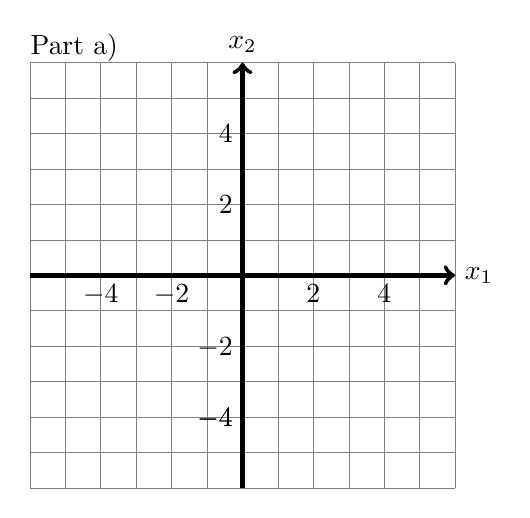
\begin{tikzpicture}[scale=.45]
        \draw[help lines, very thin, gray] (-6, -6) grid (6,6);
        \draw[ultra thick, ->] (-6, 0) -- (6, 0);
        \draw[ultra thick, ->] (0, -6) -- (0, 6);
        \node[overlay, above] at (-4.75, 5.75) { Part a)};
        \node[above] at (0, 6) {$x_2$};
        \node[right] at (6, 0) {$x_1$};
        \node[left] at (0, 2) {$2$};
        \node[below] at (2, 0) {$2$};
        \node[below] at (-2, 0) {$-2$};
        \node[left] at (0, -2.05) {$-2$};  
        \node[left] at (0, 4) {$4$};
        \node[below] at (4, 0) {$4$};
        \node[below] at (-4, 0) {$-4$};
        \node[left] at (0, -4.05) {$-4$};          
        \node[left] at (0, -4.05) {$-4$};          
        \end{tikzpicture}\qquad
        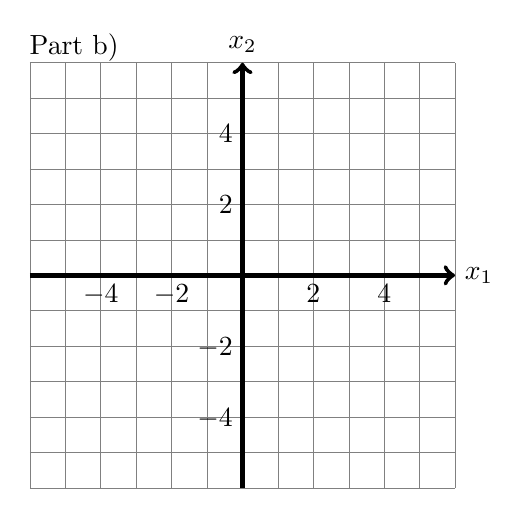
\begin{tikzpicture}[scale=.45]
        \draw[help lines, very thin, gray] (-6, -6) grid (6,6);
        \draw[ultra thick, ->] (-6, 0) -- (6, 0);
        \draw[ultra thick, ->] (0, -6) -- (0, 6);
        \node[overlay, above] at (-4.75, 5.75) { Part b) };
        \node[above] at (0, 6) {$x_2$};
        \node[right] at (6, 0) {$x_1$};
        \node[left] at (0, 2) {$2$};
        \node[below] at (2, 0) {$2$};
        \node[below] at (-2, 0) {$-2$};
        \node[left] at (0, -2.05) {$-2$};  
        \node[left] at (0, 4) {$4$};
        \node[below] at (4, 0) {$4$};
        \node[below] at (-4, 0) {$-4$};
        \node[left] at (0, -4.05) {$-4$};          
        \end{tikzpicture}
        \end{center}
        
        \vspace{24pt}
    \fi
    
    \ifnum \Solutions=1 {\color{DarkBlue} \textit{Solutions.} 
    \begin{enumerate}
        \item[a)] For eigenvalue $\lambda_1$: 
        \begin{align}
            A - \lambda_1 I = \begin{pmatrix} 4&2\\2&7 \end{pmatrix} - 4I = \begin{pmatrix} -4&2\\2&-1 \end{pmatrix}
        \end{align}
        A vector in the null space of this matrix is $v_1 = \begin{pmatrix} 1\\2\end{pmatrix}$. Any nonzero scalar multiple of this vector is also sufficient. For eigenvalue $\lambda_2$: 
        \begin{align}
            A - \lambda_2 I = \begin{pmatrix} 4&2\\2&7 \end{pmatrix}  + I = \begin{pmatrix} 1&2\\2&4 \end{pmatrix}
        \end{align}
        A vector in the null space of this matrix is $v_2 = \begin{pmatrix} -2\\1\end{pmatrix}$. Any nonzero scalar multiple of this vector is also sufficient. Sketching the spans of these vectors gives us the eigenspaces. Be sure to extend the lines to the edges of the graph, because eigenspaces are subspaces. 

        \begin{center}
        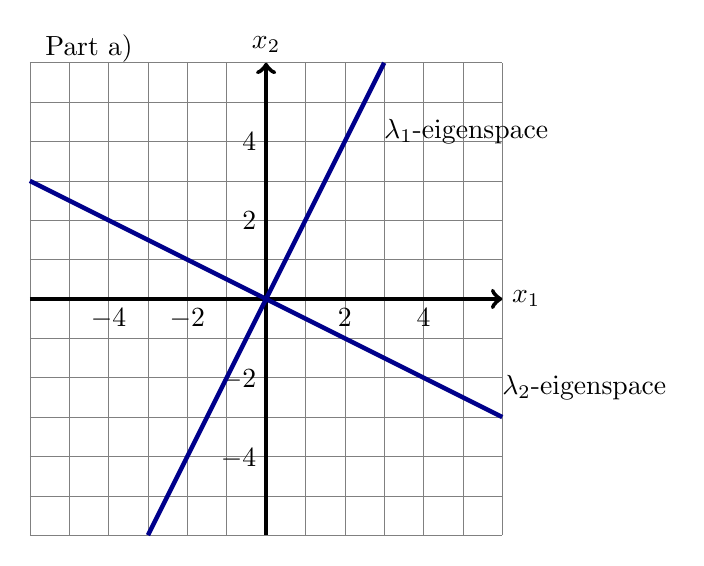
\begin{tikzpicture}[scale=.5]
        \draw[help lines, very thin, gray] (-6, -6) grid (6,6);
        \draw[ultra thick, ->] (-6, 0) -- (6, 0);
        \draw[ultra thick, ->] (0, -6) -- (0, 6);
        \node[overlay, above] at (-4.5, 5.75) {Part a)};
        \node[above] at (0, 6) {$x_2$};
        \node[right] at (6, 0) {$x_1$};
        \node[left] at (0, 2) {$2$};
        \node[below] at (2, 0) {$2$};
        \node[below] at (-2, 0) {$-2$};
        \node[left] at (0, -2.05) {$-2$};  
        \node[left] at (0, 4) {$4$};
        \node[below] at (4, 0) {$4$};
        \node[below] at (-4, 0) {$-4$};
        \node[left] at (0, -4.05) {$-4$};          
        \node[right] at (2.75,4.25) {$\lambda_1$-eigenspace};          
        \draw[ultra thick, DarkBlue,-] (-3, -6) -- (3, 6);
        \node[right] at (5.75,-2.25) {$\lambda_2$-eigenspace};          
        \draw[ultra thick, DarkBlue,-] (-6,3) -- (6,-3);        
        \end{tikzpicture}
        \end{center}
        For this particular matrix, the eigenspaces happen to be perpendicular to each other. Later in the course we will see why this is the case for this matrix. 

        \item[b)] We can approach this in a few different ways. One approach is to work out $p$ using the values of $v_1$ and $v_2$ from the previous part and then compute $Ap$: 
        \begin{align}
            Ap = A (\frac12 v_1 + 2v_2) = \begin{pmatrix} 0&2\\2&3\end{pmatrix}\left( \frac12 \begin{pmatrix} 1\\2 \end{pmatrix} +2 \begin{pmatrix} -2\\1\end{pmatrix}\right) = \begin{pmatrix} 0&2\\2&3\end{pmatrix}\begin{pmatrix} -7/2\\ 3\end{pmatrix} = \begin{pmatrix} 6\\2\end{pmatrix}
        \end{align}
        
        Or, using $Av = \lambda v$ we have that 
        \begin{align}
            Ap = A(\frac12 v_1 + 2v_2) 
            = \frac12 Av_1  + 2Av_2 
            = \frac 12 \lambda_1v_1 + 2\lambda_2v_2 
            = 2\begin{pmatrix} 1\\2 \end{pmatrix} - 2\begin{pmatrix} -2\\1 \end{pmatrix} 
            = \begin{pmatrix} 6\\2\end{pmatrix}
        \end{align}
        The vector $Ap = \begin{pmatrix} 6\\2\end{pmatrix}$ is sketched below. 
            \begin{center}
            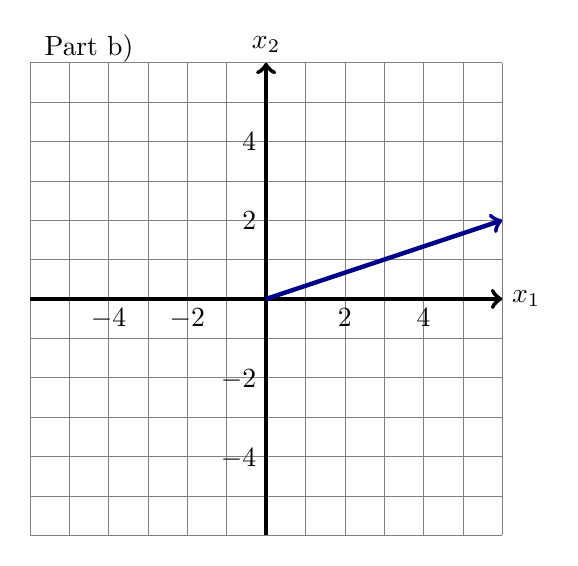
\begin{tikzpicture}[scale=.5]
            \draw[help lines, very thin, gray] (-6, -6) grid (6,6);
            \draw[ultra thick, ->] (-6, 0) -- (6, 0);
            \draw[ultra thick, ->] (0, -6) -- (0, 6);
            \node[overlay, above] at (-4.5, 5.75) {Part b)};
            \node[above] at (0, 6) {$x_2$};
            \node[right] at (6, 0) {$x_1$};
            \node[left] at (0, 2) {$2$};
            \node[below] at (2, 0) {$2$};
            \node[below] at (-2, 0) {$-2$};
            \node[left] at (0, -2.05) {$-2$};  
            \node[left] at (0, 4) {$4$};
            \node[below] at (4, 0) {$4$};
            \node[below] at (-4, 0) {$-4$};
            \node[left] at (0, -4.05) {$-4$};          
            \draw[ultra thick, DarkBlue,->] (0,0) -- (6,2);     
            \end{tikzpicture}
            \end{center}
    \end{enumerate}        
    } 

   \else
      
   \fi
\fi 



\ifnum \Version=2
    \ifnum \Solutions=1 \newpage \fi 
    
    \question[2] The $2\times 2$ matrix $A$ has eigenvalues $\lambda_1=-1$ and $\lambda_2=2$, with eigenspaces indicated in the picture. Vectors $x$ and $y$ are also shown below. Draw $A x$ and $A y$.

    \begin{center}
    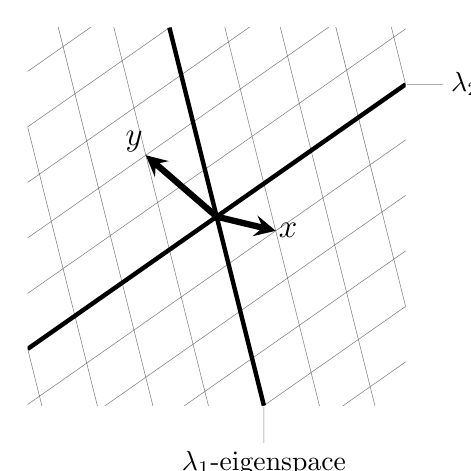
\begin{tikzpicture}[scale=.6,vectorB/.style={-stealth, black, thick, line width=0.8mm}]

      \begin{scope}
      \clip (-4, -4) rectangle (4, 4);
      \begin{scope}[cm={1,2.8/4,1/4,-1,(0,0)}]
        \draw[help lines] (-6, -6) grid (6, 6);
        \draw[vectorB] (0, 0) -- (1, 1) node[right, inner sep=0] {\large $ x$};
        \draw[vectorB] (0, 0) -- (-1, -2) node[above left, inner sep=0] {\large $ y$};
      \end{scope}
      \draw[ultra thick] (-4, -2.8) -- (4, 2.8);
      \draw[ultra thick] (-1, 4) -- (1, -4);
      \node[circle, inner sep=.4mm, fill] at (0, 0) {};
      \end{scope}
      \node[pin={[overlay, inner sep=1mm]0:{$\lambda_2$-eigenspace}}, outer sep=0, inner sep=0] at (4, 2.8) {};
      \node[pin={[overlay, inner sep=1mm]270:{$\lambda_1$-eigenspace}}, outer sep=0, inner sep=0] at (1, -4) {};
    \end{tikzpicture}
    \end{center}    
    
    \ifnum \Solutions=0
        \vspace{12pt}
    \fi

    \ifnum \Solutions=1
        {\color{DarkBlue} 
            \textbf{Solutions}\\
            Take $v_1$ to be any non-zero vector in the $\lambda_1$ eigenspace, and $v_2$ to be any non-zero vector in the $\lambda_2$-eigenspace. We could for example make the following choices for $v_1$ and $v_2$. }
            \begin{center}
            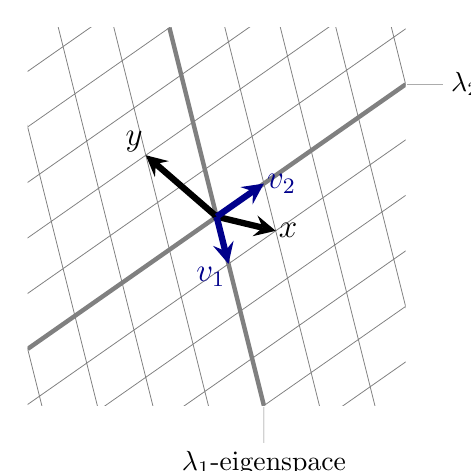
\begin{tikzpicture}[scale=.6,vectorB/.style={-stealth, black, thick, line width=0.8mm},vectorR/.style={-stealth, DarkBlue, thick, line width=0.8mm}]
                \begin{scope}
                    \clip (-4, -4) rectangle (4, 4);
                    \draw[gray,ultra thick] (-4, -2.8) -- (4, 2.8);
                    \draw[gray, ultra thick] (-1, 4) -- (1, -4);
                    \node[circle, inner sep=.4mm, fill] at (0, 0) {};              
                    \begin{scope}[cm={1,2.8/4,1/4,-1,(0,0)}]
                        \draw[help lines,line width=0.1mm] (-6, -6) grid (6, 6);
                        \draw[vectorB] (0, 0) -- (1, 1) node[right, inner sep=0] {\large $ x$};
                        \draw[vectorB] (0, 0) -- (-1, -2) node[above left, inner sep=0] {\large $ y$};
                        \draw[vectorR] (0, 0) -- (0,1) node[below left, inner sep=0] {\large $ v_1$};
                        \draw[vectorR] (0, 0) -- (1, 0) node[right, inner sep=0] {\large $ v_2$};
                    \end{scope}
                \end{scope}
                \node[pin={[overlay, inner sep=1mm]0:{$\lambda_2$-eigenspace}}, outer sep=0, inner sep=0] at (4, 2.8) {};
                \node[pin={[overlay, inner sep=1mm]270:{$\lambda_1$-eigenspace}}, outer sep=0, inner sep=0] at (1, -4) {};
            \end{tikzpicture}
            \end{center}    
            {\color{DarkBlue} 
            With this choice we have $x = v_1 + v_2$, and $y = -2v_1 - v_2$. We want to sketch $A\vec x$ and $A\vec y$, but:
            \begin{align}
                A x &= A(v_1 + v_2) = Av_1 + A v_2 = \lambda_1v_1 + \lambda_2v_2 = -v_1 + 2v_2 \\
                A y &= A(-2v_1 - v_2) = -2Av_1 - A v_2 = -2\lambda_1v_1 - \lambda_2v_2 = 2v_1 - 2v_2 
            \end{align}
            So we need to sketch $Ax = -v_1 + 2v_2$ and $Ay = 2v_1 - 2 v_2$. They are sketched below.}
            \begin{center}
            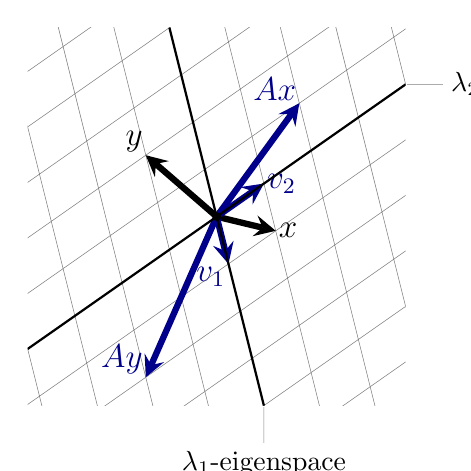
\begin{tikzpicture}[scale=.6,vectorB/.style={-stealth, black, thick, line width=0.8mm},vectorR/.style={-stealth, DarkBlue, thick, line width=0.8mm}]
              \begin{scope}
              \clip (-4, -4) rectangle (4, 4);
              \begin{scope}[cm={1,2.8/4,1/4,-1,(0,0)}]
                \draw[help lines] (-6, -6) grid (6, 6);
                \draw[vectorB] (0, 0) -- (1, 1) node[right, inner sep=0] {\large $ x$};
                \draw[vectorB] (0, 0) -- (-1, -2) node[above left, inner sep=0] {\large $ y$};
                \draw[vectorR] (0, 0) -- (0,1) node[below left, inner sep=0] {\large $ v_1$};
                \draw[vectorR] (0, 0) -- (1, 0) node[right, inner sep=0] {\large $ v_2$};                
                \draw[vectorR] (0, 0) -- (2,-1) node[above left, inner sep=0] {\large $ Ax$};
                \draw[vectorR] (0, 0) -- (-2,2) node[above left, inner sep=0] {\large $ Ay$};
              \end{scope}
              \draw[ thick] (-4, -2.8) -- (4, 2.8);
              \draw[ thick] (-1, 4) -- (1, -4);
              \node[circle, inner sep=.4mm, fill] at (0, 0) {};
              \end{scope}
              \node[pin={[overlay, inner sep=1mm]0:{$\lambda_2$-eigenspace}}, outer sep=0, inner sep=0] at (4, 2.8) {};
              \node[pin={[overlay, inner sep=1mm]270:{$\lambda_1$-eigenspace}}, outer sep=0, inner sep=0] at (1, -4) {};
            \end{tikzpicture}
            \end{center}

    \fi
\fi




\ifnum \Version=3
    \question[2] Calculate the steady state for the Markov chain shown below. Please show your work.  
        \begin{center}
        \begin{tikzpicture}[->,>=stealth',shorten >=1pt,auto,node distance=3cm,thick]
        \tikzstyle{every state}=[circle,fill=gray!10,draw,thick,,font=\bf, line width=0.4mm]
    
        \node[state] (A) {A};
        \node[state]  (B) [right of=A] {B};
        \path 
            (A) edge    [bend left] node {0.3} (B)
                edge    [loop left] node {0.7} (A)
            (B) edge    [loop right] node {0.4} (B) 
                edge    [bend left] node {0.6} (A);
        \end{tikzpicture} 
        \end{center}    

    \ifnum \Solutions=1 {\color{DarkBlue} \textit{Solutions.} 
    
        \begin{align}
            P-I &= \frac{1}{10} \begin{pmatrix} 7 & 6 \\ 3 & 4\end{pmatrix} - \begin{pmatrix} 1&0\\0&1 \end{pmatrix} = \frac{1}{10}\begin{pmatrix}-3&6\\3&-6 \end{pmatrix} \sim \begin{pmatrix}-1&2\\0&0 \end{pmatrix}
        \end{align}
        The steady-state is: 
        $$ \vec q = \frac{1}{3}\begin{pmatrix}2\\1 \end{pmatrix}$$
        } 
    \fi
\fi

\ifnum \Version=4
    \question[2] Calculate the steady state for the Markov chain shown below. Please show your work.  
        \begin{center}
        \begin{tikzpicture}[->,>=stealth',shorten >=1pt,auto,node distance=3cm,thick]
        \tikzstyle{every state}=[circle,fill=gray!10,draw,thick,,font=\bf, line width=0.4mm]
    
        \node[state] (A) {A};
        \node[state]  (B) [right of=A] {B};
        \path 
            (A) edge    [bend left] node {0.3} (B)
                edge    [loop left] node {0.7} (A)
            (B) edge    [loop right] node {0.8} (B) 
                edge    [bend left] node {0.2} (A);
        \end{tikzpicture} 
        \end{center}    

    \ifnum \Solutions=1 {\color{DarkBlue} \textit{Solutions.} 
    
        \begin{align}
            P-I &= \frac{1}{10} \begin{pmatrix} 7 & 2 \\ 3 & 8\end{pmatrix} - \begin{pmatrix} 1&0\\0&1 \end{pmatrix} = \frac{1}{10}\begin{pmatrix}-3&2\\3&-2 \end{pmatrix} \sim \begin{pmatrix}-3&2\\0&0 \end{pmatrix}
        \end{align}
        The steady-state is: 
        $$ \vec q = \frac{1}{5}\begin{pmatrix}2\\3 \end{pmatrix}$$
        } 
    \else
    \vfill         
    \fi
\fi


\ifnum \Version=5
    \question[2] Calculate the steady state for the Markov chain shown below. Please show your work.  
        \begin{center}
        \begin{tikzpicture}[->,>=stealth',shorten >=1pt,auto,node distance=3cm,thick]
        \tikzstyle{every state}=[circle,fill=gray!10,draw,thick,,font=\bf, line width=0.4mm]
    
        \node[state] (A) {A};
        \node[state]  (B) [right of=A] {B};
        \path 
            (A) edge    [bend left] node {0.3} (B)
                edge    [loop left] node {0.7} (A)
            (B) edge    [loop right] node {0.8} (B) 
                edge    [bend left] node {0.2} (A);
        \end{tikzpicture} 
        \end{center}    

    \ifnum \Solutions=1 {\color{DarkBlue} \textit{Solutions.} 
    
        \begin{align}
            P-I &= \frac{1}{10} \begin{pmatrix} 7 & 2 \\ 3 & 8\end{pmatrix} - \begin{pmatrix} 1&0\\0&1 \end{pmatrix} = \frac{1}{10}\begin{pmatrix}-3&2\\3&-2 \end{pmatrix} \sim \begin{pmatrix}-3&2\\0&0 \end{pmatrix}
        \end{align}
        The steady-state is: 
        $$ \vec q = \frac{1}{5}\begin{pmatrix}2\\3 \end{pmatrix}$$
        } 

    \fi
\fi


\ifnum \Version=6
  \TwoStateMarkov{4}{7}
\fi    

\ifnum \Version=7
    \TwoStateMarkov{7}{3} 
\fi

\ifnum \Version=8
    \TwoStateMarkov{7}{5}
\fi      



\ifnum \Version=12 % NOT NEEDED? 
    \question[2] Calculate the steady state for the Markov chain shown below. Please show your work.  
        \begin{center}
        \begin{tikzpicture}[->,>=stealth',shorten >=1pt,auto,node distance=3cm,thick]
        \tikzstyle{every state}=[circle,fill=gray!10,draw,thick,,font=\bf, line width=0.4mm]
    
        \node[state] (A) {A};
        \node[state]  (B) [right of=A] {B};
        \path 
            (A) edge    [bend left] node {0.3} (B)
                edge    [loop left] node {0.7} (A)
            (B) edge    [loop right] node {0.4} (B) 
                edge    [bend left] node {0.6} (A);
        \end{tikzpicture} 
        \end{center}    

    \ifnum \Solutions=1 {\color{DarkBlue} \textit{Solutions.} 
      Find the probability vector in the kernel of $P_I$. 
        \begin{align}
            P-I &= \frac{1}{10} \begin{pmatrix} 7 & 6 \\ 3 & 4\end{pmatrix} - \begin{pmatrix} 1&0\\0&1 \end{pmatrix} = \frac{1}{10}\begin{pmatrix}-3&6\\3&-6 \end{pmatrix} \sim \begin{pmatrix}-1&2\\0&0 \end{pmatrix}
        \end{align}
        The steady-state is: 
        $$ \vec q = \frac{1}{3}\begin{pmatrix}2\\1 \end{pmatrix}$$
        } 
    \else 
        \vfill
    \fi
\fi



\ifnum \Version=13 % NOT NEEDED? 
    \question[2] Calculate the steady state for the Markov chain shown below. Please show your work.  
        \begin{center}
        \begin{tikzpicture}[->,>=stealth',shorten >=1pt,auto,node distance=3cm,thick]
        \tikzstyle{every state}=[circle,fill=gray!10,draw,thick,,font=\bf, line width=0.4mm]
    
        \node[state] (A) {A};
        \node[state]  (B) [right of=A] {B};
        \path 
            (A) edge    [bend left] node {0.2} (B)
                edge    [loop left] node {0.8} (A)
            (B) edge    [loop right] node {0.4} (B) 
                edge    [bend left] node {0.6} (A);
        \end{tikzpicture} 
        \end{center}    

    \ifnum \Solutions=1 {\color{DarkBlue} \textit{Solutions.} 
    
        The steady state has eigenvalue 1. So it is the probability vector in the null space (i.e. - the kernel) of $P-I$. 
        \begin{align} 
            P-I &= \frac{1}{10} \begin{pmatrix} 8 & 6 \\ 2 & 4\end{pmatrix} - \begin{pmatrix} 1&0\\0&1 \end{pmatrix} = \frac{1}{10}\begin{pmatrix}-2&6\\2&-6 \end{pmatrix} \sim \begin{pmatrix}-1&3\\0&0 \end{pmatrix}
        \end{align}
        The steady-state is: 
        $$ \vec q = \frac{1}{4}\begin{pmatrix}3\\1 \end{pmatrix}$$
        } 
    \fi
\fi
        \ifnum \Solutions=0 \newpage \fi
        \question[0.25] \ID
        \ifnum \Version=0
    \question[3] $A = \begin{pmatrix}-1&1&-1\\1&-1&1\\1&-1&1 \end{pmatrix}$ has only two distinct eigenvalues, $\lambda_1 = -1$ and $\lambda_2 = 0$.   
    \begin{parts} 
        \part Construct the eigenbasis for eigenvalue $\lambda_1 = -1$. Please show your work.
        \ifnum \Solutions = 0  \vspace{6cm} \fi
        
        \part Construct the eigenbasis for eigenvalue $\lambda_2 = 0$. Please show your work.
        \ifnum \Solutions = 0  \vspace{6cm} \fi
        
        \part If possible, construct real matrices $P$ and $D$ such that $A = PDP^{-1}$, where $D$ is a diagonal matrix. 
    \end{parts}

    \ifnum \Solutions=1 {\color{DarkBlue} \textit{Solutions.} 
    \begin{enumerate}
        \item[a)] $$A - (-1) I = \begin{pmatrix} 0&1&-1\\1&0&1\\1&-1&2\end{pmatrix}\sim\begin{pmatrix} 0&1&-1\\1&0&1\\0&0&0\end{pmatrix}$$ A vector in the null space is $$v_1 = \begin{pmatrix}1\\-1\\-1 \end{pmatrix}$$ 
        \item[b)] $$A - (0) I = \begin{pmatrix} -1&1&-1\\1&-1&1\\1&-1&1\end{pmatrix}\sim\begin{pmatrix} -1&1&-1\\0&0&0\\0&0&0\end{pmatrix}$$ The first row gives us the equation $-x_1+x_2-x_3 =0$, or $x_1 = x_2 - x_3$. Vectors in the null space have the form $$x = \begin{pmatrix}x_1\\x_2\\x_3 \end{pmatrix} = \begin{pmatrix}x_2-x_3\\x_2\\x_3 \end{pmatrix} = x_2\begin{pmatrix} 1\\1\\0\end{pmatrix} + x_3 \begin{pmatrix} 1\\0\\-1\end{pmatrix}$$ 
        Two vectors that form a basis for the eigenspace are $$v_2 = \begin{pmatrix} 1\\1\\0\end{pmatrix}, \quad v_3 = \begin{pmatrix} 1\\0\\-1\end{pmatrix}$$ 
        \item[c)] $$P = \begin{pmatrix} 1&1&1\\-1&1&0\\-1&0&-1\end{pmatrix}, \quad D = \begin{pmatrix} -1&0&0\\0&0&0\\0&0&0\end{pmatrix}$$
    \end{enumerate}
    } 
   \fi
\fi 


\ifnum \Version=1
\question[3] Suppose $A = \begin{pmatrix} 5&-2\\1&3 \end{pmatrix}$. 
    \begin{parts} 
        \part Determine the eigenvalues of $A$. Show your work. 
        \ifnum \Solutions = 0 
            \vspace{4cm}
        \else
            {\color{DarkBlue} 
            $$ 0 = \det(A-\lambda I) = (5-\lambda)(3-\lambda) + 2 = \lambda^2 - 8 \lambda + 17 \ \Rightarrow \ \lambda = \frac82 \pm \frac12\sqrt{64 - 68} = 4 \pm i$$ For clarity we could set: $$\lambda_1 = 4-i, \quad \lambda_2 = 4+i$$
            }
        \fi     
        \part Determine the eigenvectors of $A$. Show your work.
        
        \ifnum \Solutions = 0 
            \vspace{2cm}
        \else
            {\color{DarkBlue} Using the symbol $\ast$ to denote a value that is not needed:
            $$(A-\lambda I) = \begin{pmatrix} 5-\lambda & -2 \\ \ast & \ast\end{pmatrix} \ \Rightarrow \ (5-\lambda)x_1 - 2x_2 = 0$$
            We covered why the second row was not needed in lecture. But as a quick reminder: the matrix $A - \lambda I$ is singular, so there can only be one pivot, so each row must be a multiple of each other (otherwise there would be two pivots and the matrix would not be singular). Then if we set $x_2 = 5 - \lambda$ we have some convenient cancellation that allows us to obtain $x_1$ quickly. 
            \begin{align}
                0 
                &= (5-\lambda)x_1 - 2x_2 \\ 
                &= (5-\lambda)x_1 - 2(5 - \lambda) \\ 
                &= x_1 - 2 \\ 
                x_1 &= 2
            \end{align}
            Then the eigenvectors have the form $\vec v = \begin{pmatrix} 2\\5 - \lambda \end{pmatrix}$. And we found that $\lambda = 4 \pm  i$, so the eigenvectors and their corresponding eigenvalues are as follows.  
            \begin{align}
                \lambda_1 &= 4-i \ \Rightarrow \vec v_1 = \begin{pmatrix} 2\\5 - \lambda_1 \end{pmatrix} = \begin{pmatrix} 2\\1+i \end{pmatrix} \\
                \lambda_2 &= 4+i \ \Rightarrow \vec v_2 = \begin{pmatrix} 2\\5-\lambda_2 \end{pmatrix} = \begin{pmatrix} 2\\1-i\end{pmatrix}
            \end{align}
            
            \textbf{Solution Notes} 
            \begin{itemize}
            \item Complex eigenvalues and eigenvectors come in conjugate pairs. So we should find that $\vec v_1$ is the conjugate of $\vec v_2$. 
            \item As you are working similar problems while preparing for an exam or completing homework, note that WolframAlpha and MATLAB are great tools for checking your work. They can give eigenvalues and eigenvectors very quickly. 
            \begin{itemize}
                \item The WolframAlpha syntax you would use to obtain the eigenvectors and eigenvalues is: \{\{5,-2\},\{1,3\}\}. Entering the matrix by itself returns the eigenvalues and eigenvectors, in addition to other information. 
                \item The MATLAB (or OCTAVE) syntax that you would use to obtain the eigenvectors and eigenvalues is: 
                [V,D] = eig([5 -2;1 3]).
            \end{itemize}
            \item You may find that your eigenvectors look very different from what the solutions present. It could be because your work is correct and your eigenvectors are a multiple of the eigenvectors that are in the solutions, and the multiple is a complex number. You can also check your work by using MATLAB or OCTAVE to compute $A\vec v - \lambda \vec v$ and see if you get the zero vector. For example, the MATLAB synatx for checking whether these calculations are correct could be (performed in one line):
            \begin{center}
                A=[5 -2;1 3], v=[2;1+i], A*v - (4-i)*v
            \end{center}
            \item Those of you going on to take a differential equations course may use these sort of calculations to construct solutions to systems of differential equations that involve complex eigenvalues. The solutions to a system of differential equations can involve calculations with complex eigenvalues. 
            \end{itemize}
            }
        \fi                  
        
    \end{parts}
\fi 


\ifnum \Version=2
    \question[3] $A = \begin{pmatrix}2&1&1\\-1&0&-1\\1&1&2 \end{pmatrix}$ has only two distinct eigenvalues, $\lambda_1 = 1$ and $\lambda_2 = 2$.   
    \begin{parts} 
        \part Construct an eigenbasis for eigenvalue $\lambda_1 = 1$. Please show your work.
        \ifnum \Solutions = 0  \vspace{6cm} \fi
        
        \part Construct an eigenbasis for eigenvalue $\lambda_2 = 2$. Please show your work.
        \ifnum \Solutions = 0  \vspace{6cm} \fi
        
        \part If possible, construct real matrices $P$ and $D$ such that $A = PDP^{-1}$, where $D$ is a diagonal matrix. 
    \end{parts}

    \ifnum \Solutions=1 {\color{DarkBlue} \textit{Solutions.} 
    \begin{enumerate}
        \item[a)] For $\lambda_1 = 1$, 
        $$A - (1) I = \begin{pmatrix} 1&1&1\\-1&-1&-1\\1&1&1\end{pmatrix}\sim\begin{pmatrix} 1&1&1\\0&0&0\\0&0&0\end{pmatrix}$$ Vectors in the null space have the form $$x = \begin{pmatrix}x_1\\x_2\\x_3 \end{pmatrix} = \begin{pmatrix}-x_2-x_3\\x_2\\x_3 \end{pmatrix} = x_2\begin{pmatrix} -1\\1\\0\end{pmatrix} + x_3 \begin{pmatrix} -1\\0\\1\end{pmatrix}$$ 
        \item[b)] For $\lambda_2 = 2$, 
        $$A - (2) I = \begin{pmatrix} 0&1&1\\-1&-2&-1\\1&1&0\end{pmatrix}\sim\begin{pmatrix} 1&1&0\\0&1&1\\0&0&0\end{pmatrix}\sim\begin{pmatrix} 1&0&-1\\0&1&1\\0&0&0\end{pmatrix}$$ Vectors in the null space have the form $$x = \begin{pmatrix}x_1\\x_2\\x_3 \end{pmatrix} = \begin{pmatrix}x_3\\-x_3\\x_3 \end{pmatrix} = x_3 \begin{pmatrix} 1\\-1\\1\end{pmatrix}$$ 
        A vector that is a basis for the eigenspace is $$v_3 = \begin{pmatrix} 1\\-1\\1\end{pmatrix}$$ But any non-zero multiple is also ok. 
        \item[c)] $$P = \begin{pmatrix} -1&-1&1\\1&0&-1\\0&1&1\end{pmatrix}, \quad D = \begin{pmatrix} 1&0&0\\0&1&0\\0&0&2\end{pmatrix}$$
    \end{enumerate}
    } 
   \fi
\fi 


\ifnum \Version=3
    \question[3] $A = \begin{pmatrix}3&1&1\\-1&1&-1\\1&1&3 \end{pmatrix}$ has only two distinct eigenvalues, $\lambda_1 = 2$ and $\lambda_2 = 3$.   
    \begin{parts} 
        \part Construct the eigenbasis for eigenvalue $\lambda_1 = 2$. Please show your work.
        \ifnum \Solutions = 0  \vspace{6cm} \fi
        
        \part Construct the eigenbasis for eigenvalue $\lambda_2 = 3$. Please show your work.
        \ifnum \Solutions = 0  \vspace{6cm} \fi
        
        \part If possible, construct real matrices $P$ and $D$ such that $A = PDP^{-1}$, where $D$ is a diagonal matrix. 
    \end{parts}

    \ifnum \Solutions=1 {\color{DarkBlue} \textit{Solutions.} 
    \begin{enumerate}
        \item[a)] For $\lambda_1 = 2$, 
        $$A - (2) I = \begin{pmatrix} 1&1&1\\-1&-1&-1\\1&1&1\end{pmatrix}\sim\begin{pmatrix} 1&1&1\\0&0&0\\0&0&0\end{pmatrix}$$ Vectors in the null space have the form $$x = \begin{pmatrix}x_1\\x_2\\x_3 \end{pmatrix} = \begin{pmatrix}-x_2-x_3\\x_2\\x_3 \end{pmatrix} = x_2\begin{pmatrix} -1\\1\\0\end{pmatrix} + x_3 \begin{pmatrix} -1\\0\\1\end{pmatrix}$$ 
        \item[b)] For $\lambda_2 = 3$, 
        $$A - (3) I = \begin{pmatrix} 0&1&1\\-1&-2&-1\\1&1&0\end{pmatrix}\sim\begin{pmatrix} 1&1&0\\0&1&1\\0&0&0\end{pmatrix}$$ Vectors in the null space have the form $$x = \begin{pmatrix}x_1\\x_2\\x_3 \end{pmatrix} = \begin{pmatrix}x_3\\-x_3\\x_3 \end{pmatrix} = x_3 \begin{pmatrix} 1\\-1\\1\end{pmatrix}$$ 
        A vector that is a basis for the eigenspace is $$v_3 = \begin{pmatrix} 1\\-1\\1\end{pmatrix}$$ But any non-zero multiple is also ok. 
        \item[c)] $$P = \begin{pmatrix} -1&-1&1\\1&0&-1\\0&1&1\end{pmatrix}, \quad D = \begin{pmatrix} 2&0&0\\0&2&0\\0&0&3\end{pmatrix}$$
    \end{enumerate}
    } 
   \fi
\fi 

\ifnum \Version=4
    \question[3] $A = \begin{pmatrix}3&1&1\\-1&1&-1\\1&1&3 \end{pmatrix}$ has only two distinct eigenvalues, $\lambda_1 = 2$ and $\lambda_2 = 3$.   
    \begin{parts} 
        \part Construct the eigenbasis for eigenvalue $\lambda_1 = 2$. Please show your work.
        \ifnum \Solutions = 0  \vspace{6cm} \fi
        
        \part Construct the eigenbasis for eigenvalue $\lambda_2 = 3$. Please show your work.
        \ifnum \Solutions = 0  \vspace{6cm} \fi
        
        \part If possible, construct real matrices $P$ and $D$ such that $A = PDP^{-1}$, where $D$ is a diagonal matrix. 
    \end{parts}

    \ifnum \Solutions=1 {\color{DarkBlue} \textit{Solutions.} 
    \begin{enumerate}
        \item[a)] For $\lambda_1 = 2$, 
        $$A - (2) I = \begin{pmatrix} 1&1&1\\-1&-1&-1\\1&1&1\end{pmatrix}\sim\begin{pmatrix} 1&1&1\\0&0&0\\0&0&0\end{pmatrix}$$ Vectors in the null space have the form $$x = \begin{pmatrix}x_1\\x_2\\x_3 \end{pmatrix} = \begin{pmatrix}-x_2-x_3\\x_2\\x_3 \end{pmatrix} = x_2\begin{pmatrix} -1\\1\\0\end{pmatrix} + x_3 \begin{pmatrix} -1\\0\\1\end{pmatrix}$$ 
        \item[b)] For $\lambda_2 = 3$, 
        $$A - (3) I = \begin{pmatrix} 0&1&1\\-1&-2&-1\\1&1&0\end{pmatrix}\sim\begin{pmatrix} 1&1&0\\0&1&1\\0&0&0\end{pmatrix}$$ Vectors in the null space have the form $$x = \begin{pmatrix}x_1\\x_2\\x_3 \end{pmatrix} = \begin{pmatrix}x_3\\-x_3\\x_3 \end{pmatrix} = x_3 \begin{pmatrix} 1\\-1\\1\end{pmatrix}$$ 
        A vector that is a basis for the eigenspace is $$v_3 = \begin{pmatrix} 1\\-1\\1\end{pmatrix}$$ But any non-zero multiple is also ok. 
        \item[c)] $$P = \begin{pmatrix} -1&-1&1\\1&0&-1\\0&1&1\end{pmatrix}, \quad D = \begin{pmatrix} 2&0&0\\0&2&0\\0&0&3\end{pmatrix}$$
    \end{enumerate}
    } 
   \fi
\fi 

\ifnum \Version=5
    \question[3] $A = \begin{pmatrix}3&1&1\\-1&1&-1\\1&1&3 \end{pmatrix}$ has only two distinct eigenvalues, $\lambda_1 = 2$ and $\lambda_2 = 3$.   
    \begin{parts} 
        \part Construct the eigenbasis for eigenvalue $\lambda_1 = 2$. Please show your work.
        \ifnum \Solutions = 0  \vspace{6cm} \fi
        
        \part Construct the eigenbasis for eigenvalue $\lambda_2 = 3$. Please show your work.
        \ifnum \Solutions = 0  \vspace{6cm} \fi
        
        \part If possible, construct real matrices $P$ and $D$ such that $A = PDP^{-1}$, where $D$ is a diagonal matrix. 
    \end{parts}

    \ifnum \Solutions=1 {\color{DarkBlue} \textit{Solutions.} 
    \begin{enumerate}
        \item[a)] For $\lambda_1 = 2$, 
        $$A - (2) I = \begin{pmatrix} 1&1&1\\-1&-1&-1\\1&1&1\end{pmatrix}\sim\begin{pmatrix} 1&1&1\\0&0&0\\0&0&0\end{pmatrix}$$ Vectors in the null space have the form $$x = \begin{pmatrix}x_1\\x_2\\x_3 \end{pmatrix} = \begin{pmatrix}-x_2-x_3\\x_2\\x_3 \end{pmatrix} = x_2\begin{pmatrix} -1\\1\\0\end{pmatrix} + x_3 \begin{pmatrix} -1\\0\\1\end{pmatrix}$$ 
        \item[b)] For $\lambda_2 = 3$, 
        $$A - (3) I = \begin{pmatrix} 0&1&1\\-1&-2&-1\\1&1&0\end{pmatrix}\sim\begin{pmatrix} 1&1&0\\0&1&1\\0&0&0\end{pmatrix}$$ Vectors in the null space have the form $$x = \begin{pmatrix}x_1\\x_2\\x_3 \end{pmatrix} = \begin{pmatrix}x_3\\-x_3\\x_3 \end{pmatrix} = x_3 \begin{pmatrix} 1\\-1\\1\end{pmatrix}$$ 
        A vector that is a basis for the eigenspace is $$v_3 = \begin{pmatrix} -1\\-1\\1\end{pmatrix}$$ But any non-zero multiple is also ok. 
        \item[c)] $$P = \begin{pmatrix} -1&-1&1\\1&0&-1\\0&1&1\end{pmatrix}, \quad D = \begin{pmatrix} 2&0&0\\0&2&0\\0&0&3\end{pmatrix}$$
    \end{enumerate}
    } 
   \fi
\fi 

\ifnum \Version=6
 \question[3] 
$A = \begin{pmatrix}-1&1&1\\2&0&2\\1&1&-1 \end{pmatrix}$ has only two distinct eigenvalues, $\lambda_1 = -2$ and $\lambda_2 = 2$.   
    \begin{parts} 
        \part Construct the eigenbasis for eigenvalue $\lambda_1 = -2$. Please show your work.
        \ifnum \Solutions = 0  \vspace{6cm} \fi
        
        \part Construct the eigenbasis for eigenvalue $\lambda_2 = 2$. Please show your work.
        \ifnum \Solutions = 0  \vspace{6cm} \fi
        
        \part If possible, construct real matrices $P$ and $D$ such that $A = PDP^{-1}$, where $D$ is a diagonal matrix. 
    \end{parts}

    \ifnum \Solutions=1 {\color{DarkBlue} \textit{Solutions.} 
    \begin{enumerate}
        \item[a)] For $\lambda_1 = -2$, 
        $$A + 2I = \begin{pmatrix} 1&1&1\\2&2&2\\1&1&1\end{pmatrix}\sim\begin{pmatrix} 1&1&1\\0&0&0\\0&0&0\end{pmatrix}$$ Vectors in the null space have the form $$x = \begin{pmatrix}x_1\\x_2\\x_3 \end{pmatrix} = \begin{pmatrix}-x_2-x_3\\x_2\\x_3 \end{pmatrix} = x_2\begin{pmatrix} -1\\1\\0\end{pmatrix} + x_3 \begin{pmatrix} -1\\0\\1\end{pmatrix}$$ 
        \item[b)] For $\lambda_2 = 2$, 
        \begin{align*}
            A - 2 I 
        &= \begin{pmatrix} -3&1&1\\2&-2&2\\1&1&-3\end{pmatrix}
        \sim\begin{pmatrix} -3&1&1\\1&-1&1\\1&1&-3\end{pmatrix}
        \sim\begin{pmatrix} -3&1&1\\1&-1&1\\0&2&-4\end{pmatrix}
        \sim\begin{pmatrix} -3&0&3\\1&0&-1\\0&1&-2\end{pmatrix} 
        \end{align*}
        We could reduce further if we like. But we can see at this point that vectors in the null space have the form $$x = \begin{pmatrix}x_1\\x_2\\x_3 \end{pmatrix} = \begin{pmatrix}x_3\\2x_3\\x_3 \end{pmatrix} = x_3 \begin{pmatrix} 1\\2\\1\end{pmatrix}$$ 
        A vector that is a basis for the eigenspace is $$v_3 = \begin{pmatrix} 1\\2\\1\end{pmatrix}$$ But any non-zero multiple of this vector would also be ok. 
        \item[c)] $$P = \begin{pmatrix} -1&-1&1\\1&0&2\\0&1&1\end{pmatrix}, \quad D = \begin{pmatrix} -2&0&0\\0&-2&0\\0&0&2\end{pmatrix}$$
    \end{enumerate}
    } \fi
\fi    
\ifnum \Version=7
\ifnum \Solutions=1 \newpage \fi
 \question[3] 
$A = \begin{pmatrix}-3&1&1\\4&0&4\\1&1&-3 \end{pmatrix}$ has only two distinct eigenvalues, $\lambda_1 = -4$ and $\lambda_2 = 2$.   
    \begin{parts} 
        \part Construct the eigenbasis for eigenvalue $\lambda_1 = -4$. Please show your work.
        \ifnum \Solutions = 0  \vspace{6cm} \fi
        
        \part Construct the eigenbasis for eigenvalue $\lambda_2 = 2$. Please show your work.
        \ifnum \Solutions = 0  \vspace{6cm} \fi
        
        \part If possible, construct real matrices $P$ and $D$ such that $A = PDP^{-1}$, where $D$ is a diagonal matrix. 
    \end{parts}

    \ifnum \Solutions=1 {\color{DarkBlue} \textit{Solutions.} 
    \begin{enumerate}
        \item[a)] For $\lambda_1 = -4$, 
        $$A + 2I = \begin{pmatrix} 1&1&1\\4&4&4\\1&1&1\end{pmatrix}\sim\begin{pmatrix} 1&1&1\\0&0&0\\0&0&0\end{pmatrix}$$ Vectors in the null space have the form $$x = \begin{pmatrix}x_1\\x_2\\x_3 \end{pmatrix} = \begin{pmatrix}-x_2-x_3\\x_2\\x_3 \end{pmatrix} = x_2\begin{pmatrix} -1\\1\\0\end{pmatrix} + x_3 \begin{pmatrix} -1\\0\\1\end{pmatrix}$$ 
        \item[b)] For $\lambda_2 = 2$, 
        $$A - 2 I = \begin{pmatrix} -5&1&1\\4&-2&4\\1&1&-5\end{pmatrix}\sim\begin{pmatrix} 0&6&-24\\0&-6&24\\1&1&-5\end{pmatrix}\sim\begin{pmatrix} 0&1&-4\\0&0&0\\1&1&-5\end{pmatrix}\sim\begin{pmatrix} 1&0&-1\\0&1&-4\\0&0&0\end{pmatrix}$$ Vectors in the null space have the form $$x = \begin{pmatrix}x_1\\x_2\\x_3 \end{pmatrix} = \begin{pmatrix} x_3\\ 4 x_3\\ x_3 \end{pmatrix} = x_3 \begin{pmatrix} 1\\ 4\\1
        \end{pmatrix}$$ 
        A vector that is a basis for the eigenspace is $v_3 = \begin{pmatrix} 1&4&1\end{pmatrix}^T$. But any non-zero multiple is also ok. 
        \item[c)] $$P = \begin{pmatrix} -1&-1&1\\1&0&4\\0&1&1\end{pmatrix}, \quad D = \begin{pmatrix} -4&0&0\\0&-4&0\\0&0&2\end{pmatrix}$$
    \end{enumerate}
    } \fi
\fi    
\ifnum \Version=8
   \question[3] 
$A = \begin{pmatrix}3&1&1\\1&3&1\\1&1&3 \end{pmatrix}$ has only two distinct eigenvalues, $\lambda_1 = 2$ and $\lambda_2 = 5$.   
    \begin{parts} 
        \part Construct the eigenbasis for eigenvalue $\lambda_1 = 2$. Please show your work.
        \ifnum \Solutions = 0  \vspace{6cm} \fi
        
        \part Construct the eigenbasis for eigenvalue $\lambda_2 = 5$. Please show your work.
        \ifnum \Solutions = 0  \vspace{6cm} \fi
        
        \part If possible, construct real matrices $P$ and $D$ such that $A = PDP^{-1}$, where $D$ is a diagonal matrix. 
    \end{parts}

    \ifnum \Solutions=1 {\color{DarkBlue} \textit{Solutions.} 
    \begin{enumerate}
        \item[a)] For $\lambda_1 = 2$, 
        $$A - 2I = \begin{pmatrix} 1&1&1\\1&1&1\\1&1&1\end{pmatrix}\sim\begin{pmatrix} 1&1&1\\0&0&0\\0&0&0\end{pmatrix}$$ Vectors in the null space have the form $$x = \begin{pmatrix}x_1\\x_2\\x_3 \end{pmatrix} = \begin{pmatrix}-x_2-x_3\\x_2\\x_3 \end{pmatrix} = x_2\begin{pmatrix} -1\\1\\0\end{pmatrix} + x_3 \begin{pmatrix} -1\\0\\1\end{pmatrix}$$ 
        \item[b)] For $\lambda_2 = 5$, 
        $$A - 5 I = \begin{pmatrix} -2&1&1\\1&-2&1\\1&1&-2\end{pmatrix}\sim\begin{pmatrix} -2&1&1\\0&-3/2&3/2\\0&0&0\end{pmatrix}$$ Vectors in the null space have the form $$x = \begin{pmatrix}x_1\\x_2\\x_3 \end{pmatrix} = \begin{pmatrix} x_1\\ x_1\\x_1 \end{pmatrix} = x_3 \begin{pmatrix} 1\\ 1\\1
        \end{pmatrix}$$ 
        A vector that is a basis for the eigenspace is $$v_3 = \begin{pmatrix} 1\\1\\1\end{pmatrix}$$ But any non-zero multiple is also ok. 
        \item[c)] $$P = \begin{pmatrix} -1&-1&1\\1&0&1\\0&1&1\end{pmatrix}, \quad D = \begin{pmatrix} 2&0&0\\0&2&0\\0&0&5\end{pmatrix}$$
    \end{enumerate}
    } \fi
\fi    



\begin{comment}
311 
464
113 

has eigenvalues 8 2 2 .  
\end{comment}



\ifnum \Version=9
    \question[3] $A = \begin{pmatrix}2&1&1\\-1&0&-1\\1&1&2 \end{pmatrix}$ has only two distinct eigenvalues, $\lambda_1 = 1$ and $\lambda_2 = 2$.   
    \begin{parts} 
        \part Construct the eigenbasis for eigenvalue $\lambda_1 = 1$. Please show your work.
        \ifnum \Solutions = 0  \vspace{6cm} \fi
        
        \part Construct the eigenbasis for eigenvalue $\lambda_2 = 2$. Please show your work.
        \ifnum \Solutions = 0  \vspace{6cm} \fi
        
        \part If possible, construct real matrices $P$ and $D$ such that $A = PDP^{-1}$, where $D$ is a diagonal matrix. 
    \end{parts}

    \ifnum \Solutions=1 {\color{DarkBlue} \textit{Solutions.} 
    \begin{enumerate}
        \item[a)] For $\lambda_1 = 1$, 
        $$A - (1) I = \begin{pmatrix} 1&1&1\\-1&-1&-1\\1&1&1\end{pmatrix}\sim\begin{pmatrix} 1&1&1\\0&0&0\\0&0&0\end{pmatrix}$$ Vectors in the null space have the form $$x = \begin{pmatrix}x_1\\x_2\\x_3 \end{pmatrix} = \begin{pmatrix}-x_2-x_3\\x_2\\x_3 \end{pmatrix} = x_2\begin{pmatrix} -1\\1\\0\end{pmatrix} + x_3 \begin{pmatrix} -1\\0\\1\end{pmatrix}$$ 
        \item[b)] For $\lambda_2 = 2$, 
        $$A - (2) I = \begin{pmatrix} 0&1&1\\-1&-2&-1\\1&1&0\end{pmatrix}\sim\begin{pmatrix} 1&1&0\\0&1&1\\0&0&0\end{pmatrix}\sim\begin{pmatrix} 1&0&-1\\0&1&1\\0&0&0\end{pmatrix}$$ Vectors in the null space have the form $$x = \begin{pmatrix}x_1\\x_2\\x_3 \end{pmatrix} = \begin{pmatrix}x_3\\-x_3\\x_3 \end{pmatrix} = x_3 \begin{pmatrix} 1\\-1\\1\end{pmatrix}$$ 
        A vector that is a basis for the eigenspace is $$v_3 = \begin{pmatrix} 1\\-1\\1\end{pmatrix}$$ But any non-zero multiple of this vector is also ok. 
        \item[c)] $$P = \begin{pmatrix} -1&-1&1\\1&0&-1\\0&1&1\end{pmatrix}, \quad D = \begin{pmatrix} 1&0&0\\0&1&0\\0&0&2\end{pmatrix}$$
    \end{enumerate}
    } 
   \fi
\fi 
    \fi 


    \ifnum \SetNumber=2
        \question[0.5] \ID
        \question[6] Fill in the blanks. You do not need to show your work. 

\begin{parts} 

% PART A DETERMINANTS AND ITS PROPERTIES 1
\part 
    \ifnum \Version=0
        If $A = \begin{pmatrix} a&b\\c&d\end{pmatrix}$ and $ B = \begin{pmatrix} 2b&2a\\d&c \end{pmatrix} $, and $ \det A = 3$, then $\det B =  \framebox{\strut\hspace{1.2cm}}$.
        
        \ifnum \Solutions=1 {\color{DarkBlue} \textit{Solution:} the answer is $-6$. Using properties of the determinant:
        \begin{align}
            3 & = \det A \\
            &= \begin{vmatrix}\begin{pmatrix} a&b\\c&d \end{pmatrix}\end{vmatrix} \\
            &= \frac12 \begin{vmatrix}\begin{pmatrix} 2a&2b\\c&d \end{pmatrix}\end{vmatrix} \\
            &= -\frac12 \begin{vmatrix}\begin{pmatrix} 2b&2a\\d&c \end{pmatrix}\end{vmatrix}, \quad \text{column swap} \\
            \begin{vmatrix}\begin{pmatrix} 2b&2a\\d&c \end{pmatrix}\end{vmatrix} & = -6
        \end{align} 
         A few notes about the solution to this problem: don't forget that column swaps change the sign of the determinant. This is because a column swap can be obtained using the sequence: transpose, row swap, transpose. And row swaps change the sign of the determinant, transposes don't change the determinant. 
        }
        \fi    
    \fi 
    \ifnum \Version=1
        If $\det A = 3$ then $\det (A^T) = \framebox{\strut\hspace{1cm}}$
        \ifnum \Solutions=1 {\color{DarkBlue} \textit{Solution:} $\text{det}A = 3$ because the determinant of a matrix does not change when the matrix is transposed. } \fi    
    \fi 
    \ifnum \Version=2
        If $a$, $b$, and $c$ are real numbers, and $A = \begin{pmatrix} a&b\\c&c\end{pmatrix}$, $ B = \begin{pmatrix}c&c\\a-2c&b-2c \end{pmatrix}$, and $ \det B = 5$, then $\det A =  \framebox{\strut\hspace{1.2cm}}$.
        \ifnum \Solutions=1 {\color{DarkBlue} \textit{Solution:} matrix $A$ can be obtained from $B$ with one row swap and by adding a multiple of a row to another row. Adding a multiple of a row to another doesn't change the determinant, and a row swap changes the sign of the determinant. So $\det A = -5$. } \fi    
    \fi 
    \ifnum \Version=3
        If $a$, $b$, and $c$ are real numbers, and $A = \begin{pmatrix} a&b\\c&c\end{pmatrix}$, $ B = \begin{pmatrix}c&c\\a-4c&b-4c \end{pmatrix}$, and $ \det A = 4$, then $\det B =  \framebox{\strut\hspace{1.2cm}}$.
        \ifnum \Solutions=1 {\color{DarkBlue} \textit{Solution:} matrix $B$ can be obtained from $A$ with one row swap and by adding a multiple of a row to another row. Adding a multiple of a row to another doesn't change the determinant, and a row swap changes the sign of the determinant. So $\det B = -4$. } \fi  
    \fi 
    \ifnum \Version=4
        If $a$, $b$, and $c$ are real numbers, and $A = \begin{pmatrix} a&b\\c&c\end{pmatrix}$, $ B = \begin{pmatrix}3c&3c\\a-4c&b-4c \end{pmatrix}$, and $ \det A = 3$, then $\det B =  \framebox{\strut\hspace{1.2cm}}$.
        \ifnum \Solutions=1 {\color{DarkBlue} \textit{Solution:} matrix $B$ can be obtained from $A$ with one row swap, scaling a row by 3, and by adding a multiple of a row to another row. Adding a multiple of a row to another doesn't change the determinant, scaling a row by 3 multiplies the determinant by 3, and a row swap changes the sign of the determinant. So $\det B = -9$. } \fi  
    \fi 
    \ifnum \Version=5
        If $a$, $b$, and $c$ are real numbers, and $A = \begin{pmatrix} a&b\\c&c\end{pmatrix}$, $ B = \begin{pmatrix}c&c\\a-4c&b-4c \end{pmatrix}$, and $ \det A = 3$, then $\det B =  \framebox{\strut\hspace{1.2cm}}$.
        \ifnum \Solutions=1 {\color{DarkBlue} \textit{Solution:} matrix $B$ can be obtained from $A$ with one row swap and by adding a multiple of a row to another row. Adding a multiple of a row to another doesn't change the determinant, and a row swap changes the sign of the determinant. So $\det B = -3$. } \fi  
    \fi 
    \ifnum \Version=6
      If  $c \in \mathbb R$,  $A = \begin{pmatrix} 5&4\\c&c\end{pmatrix}$, $ B = \begin{pmatrix}2c&2c\\5-4c&4-4c \end{pmatrix}$, and $ \det A = 3$, then $\det B =  \framebox{\strut\hspace{1.2cm}}$.
        \ifnum \Solutions=1 {\color{DarkBlue} \textit{Solution:} matrix $B$ can be obtained from $A$ with one row swap and by adding a multiple of a row to another row. And multiplying a column by $2$.  Adding a multiple of a row to another doesn't change the determinant, and a row swap changes the sign of the determinant. Multiplying a column by $2$ multiplies the determinant by $2$. So $\det B = -6$. }
        \fi
    \fi    
    \ifnum \Version=7
              If  $c$ is a  real number,  $A = \begin{pmatrix} 5&4\\c&c\end{pmatrix}$, $ B = \begin{pmatrix}10& c\\8 & c  \end{pmatrix}$, and $ \det A = 4$, then $\det B =  \framebox{\strut\hspace{1.2cm}}$.
        \ifnum \Solutions=1 {\color{DarkBlue} \textit{Solution:} matrix $B$ can be obtained from $A$ taking a transpose,  and multiplying a column by $2$. A tranpose does not change the determinant.  Multiplying a column by $2$ multiplies the determinant by $2$. So $\det B = 8$. }
        
         \fi
    \fi    
    \ifnum \Version=8
              If  $c$ is a  real number,  $A = \begin{pmatrix} 7&c \\2&c\end{pmatrix}$, $ B = \begin{pmatrix}  c+7 &21 \\c+2&6 \end{pmatrix}$, and $ \det A = 5$, then $\det B =  \framebox{\strut\hspace{1.2cm}}$.
        \ifnum \Solutions=1 {\color{DarkBlue} \textit{Solution:} matrix $B$ can be obtained from $A$ with one row swap and by adding a multiple of a row to another row. And multiplying a column by $3$.  Adding a multiple of a row to another doesn't change the determinant, and a row swap changes the sign of the determinant. Multiplying a column by $3$ multiplies the determinant by $3$. So $\det B = -15$. }
             \fi
    \fi          







% PART B CALCULATE A DETERMINANT
\part 
    \ifnum \Version=0
        The determinant of $A = \begin{pmatrix}  1&2&3\\1&2&3\\1&2&3\end{pmatrix}$ is: $\framebox{\strut\hspace{1.2cm}}$.
        
        \ifnum \Solutions=1 {\color{DarkBlue} \textit{Solution:} by inspection the matrix has dependent columns, so the matrix is singular. The determinant of a singular matrix is zero. So it isn't necessary to compute the determinant using a co-factor expansion.} \fi    
    \fi 
    \ifnum \Version=1
        The determinant of $A = \begin{pmatrix} 2&3\\0&-3\end{pmatrix}$ is equal to \framebox{\strut\hspace{1cm}}.
        \ifnum \Solutions=1 {\color{DarkBlue} \textit{Solution:} $\det A = 2\cdot (-3) = -6$. The matrix is triangular so the determinant is the product of the entries on the diagonal. } \fi    
    \fi 
    \ifnum \Version=2
        The determinant of $A = \begin{pmatrix} 2&0&0\\4&3&0\\12&-3&4\end{pmatrix}$ is equal to \framebox{\strut\hspace{1cm}}.
        \ifnum \Solutions=1 {\color{DarkBlue} \textit{Solution:} $\det A = 2\cdot 3 \cdot 4= 24$. The matrix is triangular so the determinant is the product of the entries on the diagonal. } \fi    
    \fi 
    \ifnum \Version=3
        The determinant of $A = \begin{pmatrix} 2&0\\4&5\end{pmatrix}$ is equal to \framebox{\strut\hspace{1cm}}.
        \ifnum \Solutions=1 {\color{DarkBlue} \textit{Solution:} $\det A = 2\cdot 5 = 10$. The matrix is triangular so the determinant is the product of the entries on the diagonal.  } \fi    
    \fi 
    \ifnum \Version=4
        The determinant of $A = \begin{pmatrix} 2&0\\4&6\end{pmatrix}$ is equal to \framebox{\strut\hspace{1cm}}.
        \ifnum \Solutions=1 {\color{DarkBlue} \textit{Solution:}  $\det A = 2\cdot 6 = 12$. The matrix is triangular so the determinant is the product of the entries on the diagonal. } \fi    
    \fi 
    \ifnum \Version=5
        The determinant of $A = \begin{pmatrix} 2&0\\4&-4\end{pmatrix}$ is equal to \framebox{\strut\hspace{1cm}}.
        \ifnum \Solutions=1 {\color{DarkBlue} \textit{Solution:} $\det A = 2\cdot (-4) = -8$. The matrix is triangular so the determinant is the product of the entries on the diagonal.  } \fi    
    \fi 
    \ifnum \Version=6
        Suppose $\det A = \begin{pmatrix} 2& c\\4&3\end{pmatrix}=14$. 
        Then $c = \framebox{\strut\hspace{1cm}}$. 
        \ifnum \Solutions=1 {\color{DarkBlue} \textit{Solution:}  calculate the determinant: \begin{align}
            14 &= |A| = 6 -4c \\ 4c &= -8 \\ c &= -2
        \end{align}So $c = -2$. } \fi    
    \fi 
    
    \ifnum \Version=7
        The determinant of $A = \begin{pmatrix}  1&2&0\\1&2&0\\1&2&1\end{pmatrix}$ is: $\framebox{\strut\hspace{1.2cm}}$.
        
        \ifnum \Solutions=1 {\color{DarkBlue} \textit{Solution:} by inspection the matrix has dependent columns, so the matrix is singular. The determinant of a singular matrix is zero. So it isn't necessary to compute the determinant using a co-factor expansion.}
          \fi
    \fi    
    \ifnum \Version=8
        The determinant of $A = \begin{pmatrix}  1&0&3\\1&0&3\\1&2&3\end{pmatrix}$ is: $\framebox{\strut\hspace{1.2cm}}$.
        
        \ifnum \Solutions=1 {\color{DarkBlue} \textit{Solution:} by inspection the matrix has dependent columns, so the matrix is singular. The determinant of a singular matrix is zero. So it isn't necessary to compute the determinant using a co-factor expansion.}
        \fi
    \fi      

% PART C DETERMINANT AND TRANSFORM 
\part 
    \ifnum \Version=0
        Suppose $A$ is a $2\times 2$ matrix and $T_A = A\vec x$ is a linear transformation that first rotates vectors in $\mathbb R^2$ clockwise about the origin by $\pi/2$ radians, then reflects them across the $x_2$-axis. Then det$A$ = \framebox{\strut\hspace{1cm}}.
        
        \ifnum \Solutions=1 {\color{DarkBlue} \textit{Solution:} by inspection $\det A = -1$ because the standard matrix of the transform is $A = A_{reflect}A_{rotate}$ and $\det A = \det (A_{reflect}A_{rotate}) = \det A_{reflect} \det A_{rotate} = (-1)(1) = -1$.}\fi
    \fi 
    \ifnum \Version=1
        Suppose $A$ is a $2\times 2$ matrix and $T_A = A\vec x$ is a linear transformation that first rotates vectors in $\mathbb R^2$ counterclockwise by $\pi/2$ radians about the origin, then projects them onto the $x_1$-axis. Then det$A$ = \framebox{\strut\hspace{1cm}}.
        
        \ifnum \Solutions=1 {\color{DarkBlue} \textit{Solution:}  $\det A = 0$. The determinant of a projection is zero. And the standard matrix of the transform is $A = A_{\textup{project}}A_{\textup{rotate}}$ and $\det A = \det (A_{\textup{project}}A_{\textup{rotate}}) = \det A_{\textup{project}} \det A_{\textup{rotate}}  = (0)(1) = 0$.} \fi    
    \fi 
    \ifnum \Version=2
        Suppose $A$ is a $2\times 2$ matrix and $T_A = A\vec x$ is a linear transformation that first rotates vectors in $\mathbb R^2$ counterclockwise by $\pi/2$ radians about the origin, then reflects them across the $x_2$-axis. Then det$A$ = \framebox{\strut\hspace{1cm}}.
        \ifnum \Solutions=1 {\color{DarkBlue} \textit{Solution:} by inspection $\det A = -1$ because the standard matrix of the transform is $A = A_{\textup{reflect}}A_{\textup{rotate}}$ and $\det A = \det (A_{\textup{reflect}}A_{\textup{rotate}}) = \det A_{\textup{reflect}} \det A_{\textup{rotate}} = (-1)(1) = -1$.} \fi    
    \fi 
    \ifnum \Version=3
        Suppose $A$ is a $2\times 2$ matrix and $T_A = A\vec x$ is a linear transformation that first projects vectors in $\mathbb R^2$ onto the $x_1$-axis, then reflects them across the $x_2$-axis. Then det$A$ = \framebox{\strut\hspace{1cm}}.
        \ifnum \Solutions=1 {\color{DarkBlue} \textit{Solution:}  $\det A = 0$, since there is a projection. The standard matrix of the transform is $A = A_{\textup{reflect}}A_{\textup{proj}}$ and $\det A = \det (A_{\textup{reflect}}A_{\textup{proj}}) = \det A_{\textup{reflect}} \det A_{\textup{proj}} = (-1)(0) = 0$.}\fi    
    \fi 
    \ifnum \Version=4
        $R$ is the parallelogram determined by $\vec p_1 = \begin{pmatrix}3\\4 \end{pmatrix}$, and $\vec p_2 = \begin{pmatrix} 2\\2\end{pmatrix}$.  If $A = \begin{pmatrix} 1&-1\\1&1\end{pmatrix}$, the area of the image of $R$ under the map $ \vec x\mapsto A\vec x$ is \framebox{\strut\hspace{1cm}}.
        \ifnum \Solutions=1 {\color{DarkBlue} \textit{Solution:} 
        The parallelogram has area $2$, and the matrix has determinant $2$, so the area is $4$.} \fi    
    \fi 
    \ifnum \Version=5
        $R$ is the parallelogram determined by $\vec p_1 = \begin{pmatrix}3\\4 \end{pmatrix}$, and $\vec p_2 = \begin{pmatrix} 2\\2\end{pmatrix}$.  If $A = \begin{pmatrix} 1&-1\\1&4\end{pmatrix}$, then $\det A = \framebox{\strut\hspace{1cm}}$, and the area of the image of $R$ under the map $ \vec x\mapsto A\vec x$ is \framebox{\strut\hspace{1cm}}.
        \ifnum \Solutions=1 {\color{DarkBlue} \textit{Solution:} The determinant of $A$ is $$\det A = \begin{vmatrix} 1&-1\\1&4 \end{vmatrix} = 5$$ The parallelogram has area equal to $$\begin{vmatrix} 3&2\\4&2 \end{vmatrix} = 6-8 = -2$$ The matrix has determinant $5$, so the area is $| -2 \cdot 5| = |-10| = 10$. No partial credit for writing that the area is $-10$. Area cannot be negative. } \fi    
    \fi 
    \ifnum \Version=6
    Suppose $A$ is a $2\times 2$ matrix and $T_A = A\vec x$ is a linear transformation that first reflects vectors in $\mathbb R^2$ across the $x_1$-axis, then reflects them across the $x_2$-axis. Then det$A$ = \framebox{\strut\hspace{1cm}}.
        \ifnum \Solutions=1 {\color{DarkBlue} \textit{Solution:}  $\det A = 1$, since each reflection matrix has determinant $-1$. The standard matrix of the transform is given by $ A e_1 = -e_1 $ and $A e_2 = -e_2$.}    
    \fi
    \fi    
    \ifnum \Version=7
         Suppose $A$ is a $2\times 2$ matrix and $T_A = A\vec x$ is a linear transformation that first rotates vectors in $\mathbb R^2$ counterclockwise by $\pi/4$ radians about the origin, then reflects them across the $x_1$-axis. Then det$A$ = \framebox{\strut\hspace{1cm}}.
        \ifnum \Solutions=1 {\color{DarkBlue} \textit{Solution:} by inspection $\det A = -1$ because the standard matrix of the transform is $A = A_{\textup{reflect}}A_{\textup{rotate}}$ and $\det A = \det (A_{\textup{reflect}}A_{\textup{rotate}}) = \det A_{\textup{reflect}} \det A_{\textup{rotate}} = (-1)(1) = -1$.}
        \fi
    \fi    
    \ifnum \Version=8
        $R$ is the parallelogram determined by $\vec p_1 = \begin{pmatrix}3\\1 \end{pmatrix}$, and $\vec p_2 = \begin{pmatrix} 2\\2\end{pmatrix}$.  If $A = \begin{pmatrix} 1&-1\\1&1\end{pmatrix}$, the area of the image of $R$ under the map $ \vec x\mapsto A\vec x$ is \framebox{\strut\hspace{1cm}}.
        \ifnum \Solutions=1 {\color{DarkBlue} \textit{Solution:} 
        The parallelogram has area $4$, and the matrix has determinant $2$, so the area is $8$.}
        \fi 
        
    \fi      

% D DETERMINANT PROPERTIES (eg det(AB)=det(A)det(B))
\part 
    \ifnum \Version=0
        $S$ is the parallelogram determined by $\vec v_1 = \begin{pmatrix} 4\\5\end{pmatrix}$, and $\vec v_2 =\begin{pmatrix}3\\4 \end{pmatrix}$.  If $A = \begin{pmatrix}2&2 \\5&3 \end{pmatrix}$, the area of the image of $S$ under the map $ \vec x\mapsto A\vec x$ is $\framebox{\strut\hspace{1cm}}$.  
        
        \ifnum \Solutions=1 {\color{DarkBlue} \textit{Solution:} The area will be the absolute value of $\det \left(AB \right)$ where $B=\begin{pmatrix} \vec v_1 & \vec v_2\end{pmatrix}$. Then $$
        \begin{vmatrix} \det \left( AB \right) \end{vmatrix}
        = \begin{vmatrix} \det \left(\begin{pmatrix} 4&3\\5&4\end{pmatrix}\begin{pmatrix} 2&2 \\5&3\end{pmatrix} \right) \end{vmatrix}
        = \left| \, \begin{vmatrix} 4&3\\5&4\end{vmatrix}\begin{vmatrix} 2&2 \\5&3\end{vmatrix}\, \right|
        = \begin{vmatrix} (16-15)(6-10)\end{vmatrix}
        = 4$$ Don't forget that area is non-negative, so we need to take the absolute value.} 
        \fi    
    \fi 
    \ifnum \Version=1
        If $A$ and $B$ are $n\times n$ matrices, $\det A = -3$, and $\det B= 2$, then $\det(AB^2) = \framebox{\strut\hspace{1cm}}$.
        \ifnum \Solutions=1 {\color{DarkBlue} \textit{Solution:} $\det(AB^2) = \det A \det B \det B = -12$. } \fi    
    \fi 
    \ifnum \Version=2
        A $2\times 2$ matrix $A$ has columns $\vec a_1$, $\vec a_2$, so that $A = (\vec a_1 \ \ \vec a_2)$. If $\det(A) = 3$, and matrix $B = (\vec a_2 \ \ 2\vec a_1)$, then $\det(B) = \framebox{\strut\hspace{1.2cm}}$
        \ifnum \Solutions=1 {\color{DarkBlue} \textit{Solution:} $-6$ because a column swap changes the determinant by a factor of $-1$ and the factor of 2 will increase the determinant by a factor of 2.  } \fi    
    \fi 
    \ifnum \Version=3
        If $A$, $B$, and $C$ are $n\times n$ matrices, $\det A = -1$, $\det B = 2$, and $\det(BC) = 4$, then $\det(AB^2C) = \framebox{\strut\hspace{1cm}}$.
        \ifnum \Solutions=1 {\color{DarkBlue} \textit{Solution:} $-8$ because $\det(AB^2C) = (\det A) (\det B) (\det BC) = - 8$. } \fi    
    \fi 
    \ifnum \Version=4
        A $2\times 2$ matrix $A$ has columns $\vec a_1$, $\vec a_2$, so that $A = (\vec a_1 \ \ \vec a_2)$. If $\det(A) = 4$, and matrix $B = (\vec a_2 \ \ 3\vec a_1)$, then $\det(B) = \framebox{\strut\hspace{1.2cm}}$
        \ifnum \Solutions=1 {\color{DarkBlue} \textit{Solution:} $-12$ because a column swap changes the determinant by a factor of $-1$ and the factor of 3 will increase the determinant by a factor of 3. No partial credit. } \fi  
    \fi 
    \ifnum \Version=5
        If $A$, $B$, and $C$ are $n\times n$ matrices, $\det A = -1$, $\det B = 2$, and $\det(BC) = 5$, then $\det(AB^2C) = \framebox{\strut\hspace{1cm}}$.
        \ifnum \Solutions=1 {\color{DarkBlue} \textit{Solution:} $-10$ because $\det(AB^2C) = (\det A) (\det B) (\det BC) = (-1)(2)(5) = - 10$. } \fi    
    \fi 
    \ifnum \Version=6
        If $A$, $B$, and $C$ are $n\times n$ matrices, $\det A = -3$, $\det B = 2$, and $\det(BC) = -5$, then $\det(AB^2C) = \framebox{\strut\hspace{1cm}}$.
        \ifnum \Solutions=1 {\color{DarkBlue} \textit{Solution:} $30$ because $\det(AB^2C) = (\det A) (\det B) (\det BC) = 30$. }\fi
    \fi    
    \ifnum \Version=7
        If $A$, $B$, and $C$ are $n\times n$ matrices, $\det A = -1$, $\det B = 2$, and $\det(BC) = -5$, then $\det(AB^2C^T) = \framebox{\strut\hspace{1cm}}$.
        \ifnum \Solutions=1 {\color{DarkBlue} \textit{Solution:} $10$ because $\det(AB^2C^T) = (\det A) (\det B) (\det BC) = (-1)(2)(-5) = 10$. } \fi
    \fi    
    \ifnum \Version=8
       A $3\times 3$ matrix $A$ has columns $\vec a_1$, $\vec a_2$, $\vec a_3$, so that $A = (\vec a_1 \ \ \vec a_2\ \ \vec a_3)$. If $\det(A) = 4$, and matrix $B = (3\vec a_2 \ \ \vec a_1 \ \ 2\vec a_3)$, then $\det(B) = \framebox{\strut\hspace{1.2cm}}$
        \ifnum \Solutions=1 {\color{DarkBlue} \textit{Solution:} $-24$ because a column swap changes the determinant by a factors of $2$ and $3$ will increase the determinant by a factor of $2\cdot 3 = 6$.  } \fi
    \fi      










% E SOMETHING RELATED TO CHARACTERISITC POLYNOMIAL
\part 
    \ifnum \Version=0
        If $A$ is a $2\times 2$ matrix whose characteristic polynomial is $\lambda ^2 - 5\lambda + 6$, then the eigenvalues of $A$ are $\lambda_1 = \framebox{\strut\hspace{1cm}}$ and $\lambda_2 = \framebox{\strut\hspace{1cm}}$. 
        
        \ifnum \Solutions=1 {\color{DarkBlue} \textit{Solution:} Factoring yields $\lambda ^2 - 5\lambda + 6 = (\lambda - 2)(\lambda - 3)$. Thus the roots are 2 and 3 and the eigenvalues are $$\lambda_1 = 2, \lambda_2 = 3$$ It would also be correct to write $$\lambda_1 = 3, \lambda_2 = 2$$ There is no requirement for the first eigenvalue to be the largest or smallest eigenvalue of the matrix.  } \fi    
    \fi 
    \ifnum \Version=1
        If $A$ is a $2\times 2$ matrix whose characteristic polynomial is $\lambda ^2 - 6\lambda + k$, then $A$ has exactly one eigenvalue with algebraic multiplicity 2 when $k = \framebox{\strut\hspace{1cm}}$. 
        
        \ifnum \Solutions=1 {\color{DarkBlue} \textit{Solution:} quadratic equation for roots of the polynomial yields $$\lambda = \frac{6}{2} \pm \frac12 \sqrt{(-6)^2 - 4\cdot 1 \cdot k} = 3 \pm \frac12 \sqrt{36 - 4 k}$$ Thus the roots are repeated when $k=9$. So when $k=9$, the matrix has one eigenvalue with algebraic multiplicity 2. For all other values of $k$ the eigenvalues are distinct.  } \fi    
    \fi 
    \ifnum \Version=2
        If $A$ is a $2\times 2$ matrix whose characteristic polynomial is $\lambda ^2 + k\lambda + 9$, then $A$ has complex eigenvalues with a non-zero imaginary component when $\framebox{\strut\hspace{1cm}} < k < \framebox{\strut\hspace{1cm}}$. 
        
        \ifnum \Solutions=1 {\color{DarkBlue} \textit{Solution:} quadratic equation for roots of the polynomial yields $$\lambda = \frac{-k}{2} \pm \frac12 \sqrt{(k)^2 - 4\cdot 1 \cdot 9} = 3 \pm \frac12 \sqrt{k^2 - 36}$$ Thus the roots are complex when $k^2 - 36 < 0$, which is when $|k| < 6$. So when $-6 < k < 6$, the matrix has complex eigenvalues with an imaginary component that is non-zero. For all other values of $k$ the eigenvalues are real.  } \fi    
    \fi 
    \ifnum \Version=3
        If $A$ is a square matrix whose characteristic polynomial is $\lambda (\lambda - 5)$, then the $A$ has $\framebox{\strut\hspace{1cm}}$ columns, $\det A = \framebox{\strut\hspace{1cm}}$, and the eigenvalues of $A$ are \framebox{\strut\hspace{1cm}} and \framebox{\strut\hspace{1cm}}.  
        \ifnum \Solutions=1 {\color{DarkBlue} \textit{Solution:} there are exactly two roots, so the corresponding matrix must be $2\times 2$ (hence there are two columns). One of the eigenvalues is zero, so the determinant of the matrix is also zero. The eigenvalues are $0$ and $5$, and we could put them either order. In other words, there is no requirement that the first eigenvalue be zero and the second eigenvalue be 5.  } \fi    
    \fi 
    \ifnum \Version=4
        If the characteristic polynomial of a square $2\times2$ matrix is $\lambda^2 -2\lambda -3 - k$, then one of the eigenvalues of $A$ is zero when $k = \framebox{\strut\hspace{1cm}}$ and $A$ has an eigenvalue with algebraic multiplicity 2 when $k = \framebox{\strut\hspace{1cm}}$. 
        \ifnum \Solutions=1 {\color{DarkBlue} \textit{Solution:} Using the quadratic equation for the roots:
        \begin{align}
            \lambda = \frac{2}{2} \pm \frac12 \sqrt{2^2 - 4(-3-k)} = 1 \pm \frac12 \sqrt{16 + 4k} = 1 \pm \sqrt{4 + k}
        \end{align}
        So one of the eigenvalues is zero when 
        \begin{align}
            0 &= 1 - \sqrt{4 + k} \quad \Rightarrow \quad k = -3
        \end{align} And $A$ has a repeated eigenvalue with algebraic multiplicity when $4+k=0$, or when $k = -4$.} \fi    
    \fi 
    \ifnum \Version=5
        If $A$ is a $2\times 2$ matrix whose characteristic polynomial is $\lambda ^2 - 5\lambda + 4$, then the eigenvalues of $A$ are $\lambda_1 = \framebox{\strut\hspace{1cm}}$ and $\lambda_2 = \framebox{\strut\hspace{1cm}}$. 
        \ifnum \Solutions=1 {\color{DarkBlue} \textit{Solution:} factoring yields $\lambda ^2 + 7\lambda + 12 = (\lambda - 4)(\lambda -1)$. Thus the roots are 4 and 1 and the eigenvalues are $$\lambda_1 = 4, \lambda_2 = 1$$ It would also be correct to write $$\lambda_1 = 1, \lambda_2 = 4$$ There is no requirement for the first eigenvalue to be the largest or smallest. } 
        \fi    
    \fi 
    \ifnum \Version=6
    If $A$ is a $2\times 2$ matrix whose characteristic polynomial is $\lambda ^2 - 6\lambda + 8$, then the eigenvalues of $A$ are $\lambda_1 = \framebox{\strut\hspace{1cm}}$ and $\lambda_2 = \framebox{\strut\hspace{1cm}}$. 
        \ifnum \Solutions=1 {\color{DarkBlue} \textit{Solution:} factoring yields $\lambda ^2 + 6\lambda + 8 = (\lambda - 4)(\lambda -2)$. Thus the roots are 4 and 2 and the eigenvalues are $$\lambda_1 = 4, \lambda_2 = 2$$ It would also be correct to write $$\lambda_1 = 2, \lambda_2 = 4$$ There is no requirement for the first eigenvalue to be the largest or smallest. }
        \fi
    \fi    
    \ifnum \Version=7
    If $A$ is a $2\times 2$ matrix whose characteristic polynomial is $\lambda ^2 - \lambda -12$, then the eigenvalues of $A$ are $\lambda_1 = \framebox{\strut\hspace{1cm}}$ and $\lambda_2 = \framebox{\strut\hspace{1cm}}$. 
        \ifnum \Solutions=1 {\color{DarkBlue} \textit{Solution:} factoring yields $\lambda ^2 - \lambda -12 = (\lambda - 4)(\lambda +3)$. Thus the roots are 4 and $-3$ and the eigenvalues are $\lambda_1 = 4, \lambda_2 = -3$. It would also be correct to write $$\lambda_1 = -3, \lambda_2 = 4$$ There is no requirement for the first eigenvalue to be the largest or smallest eigenvalue of the matrix. }
        \fi
    \fi    
    \ifnum \Version=8
        If the characteristic polynomial of a square $2\times2$ matrix is $\lambda^2 -4\lambda +2 + k$, then one of the eigenvalues of $A$ is zero when $k = \framebox{\strut\hspace{1cm}}$ and $A$ has an eigenvalue with algebraic multiplicity 2 when $k = \framebox{\strut\hspace{1cm}}$. 
        \ifnum \Solutions=1 {\color{DarkBlue} \textit{Solution:} Using the quadratic equation for the roots:
        \begin{align}
            \lambda = \frac{4}{2} \pm \frac12 \sqrt{4^2 - 4(2+k)} = 2 \pm \frac12 \sqrt{8 - 4k} = 2 \pm \sqrt{2 - k}
        \end{align}
        So one of the eigenvalues is zero when $k = -2$. And $A$ has a repeated eigenvalue with algebraic multiplicity when $2-k=0$, or when $k = 2$.} \fi    
    \fi      

    % GOOD PROBLEM WE DIDN'T USE IN 2023
    \ifnum \Version=9
    If $A = \begin{pmatrix} 1&k\\5&7\end{pmatrix}$, and the roots of the characteristic polynomial, $p(\lambda)$, are $\lambda_1=6$ or $\lambda_2=2$, then $k= \framebox{\strut\hspace{1cm}}$. 
    
        \ifnum \Solutions=1 {\color{DarkBlue} \textit{Solution:} the determinant of $A-\lambda I$ is the characteristic polynomial $$p = (1-\lambd)(7-\lambda) -5k = \lambda^2 -8\lambda +7-5k$$ But the roots of the characteristic polynomial are 6 and 2, so $$p(\lambda) = (\lambda - 2)(\lambda - 6) = \lambda^2 -8\lambda + 12$$ Comparing the two expressions for $p$, we obtain
        $$12 = 7 - 5k$$
        So $k = -1$. 
        } \fi
    \fi

% F GEOMETRIC MULTIPLICITY, DIAGONALIZABILITY, OR AV=λV
\part 
    \ifnum \Version=0
        Suppose $A$ is a diagonalizable $5\times 5$ matrix and $\det (A - \lambda I) =  (\lambda -4)^2(\lambda-6)^3$. Then $4$ is an eigenvalue of $A$ that has algebraic multiplicity \framebox{\strut\hspace{1cm}} and geometric multiplicity \framebox{\strut\hspace{1cm}}.  
        \ifnum \Solutions=1 {\color{DarkBlue} \textit{Solution:} The algebraic multiplicity of the eigenvalue $\lambda = 4$ is the number of times the eigenvalue repeats as a root of the characteristic polynomial, which is 2. When a matrix is diagonalizable the geometric and algebraic multiplicities are equal, so the geometric multiplicity is also 2.  } \fi    
    \fi 
    \ifnum \Version=1
        If $A = \begin{pmatrix} a_{11}&a_{12}\\a_{21}&a_{22}\end{pmatrix}$ is a $2\times 2$ matrix in echelon form whose eigenvalues are equal to 4 and 1 then $a_{11} = \framebox{\strut\hspace{1cm}}$, $a_{21} = \framebox{\strut\hspace{1cm}}$, $a_{22} = \framebox{\strut\hspace{1cm}}$.
        
        \ifnum \Solutions=1 {\color{DarkBlue} \textit{Solution:} a possible solution to this question is \begin{align}
            a_{11} = 1,  a_{21} = 0, a_{22}=4
        \end{align} 
        and the only other possible solution is \begin{align}
            a_{11} = 4,  a_{21} = 0, a_{22}=1
        \end{align} 
        
        } \fi    
    \fi 

    \ifnum \Version=2
        If $A$ has eigenvector $v = \begin{pmatrix} 2\\3 \end{pmatrix}$ with corresponding eigenvalue $\lambda = 2$, then $A^2v = \begin{pmatrix} c_1\\c_2\end{pmatrix}$, where $c_1 = \framebox{\strut\hspace{1cm}}$, $c_2 = \framebox{\strut\hspace{1cm}}$. 
        \ifnum \Solutions=1 {\color{DarkBlue} \textit{Solution:} If $\lambda = 2$ is an eigenvalue of $A$, then $A(Av) = A(\lambda v)$ becomes $A^2v = \lambda^2v$, and $\lambda^2 = 4$, so $A^2v = 4 v = \begin{pmatrix} 8\\12\end{pmatrix}$.   } \fi    
    \fi 
    \ifnum \Version=3
        If $\lambda = 2$ is an eigenvalue of $A$, then an eigenvalue of $A^2$ is \framebox{\strut\hspace{1cm}}. 
        \ifnum \Solutions=1 {\color{DarkBlue} \textit{Solution:} 4, because if $\lambda = 2$ is an eigenvalue of $A$, then for some $v$, we will have $Av=2v$. So $A(Av) = A(\lambda v)$ becomes $A^2v = \lambda^2v$, and $\lambda^2 = 2^2=4$ is an eigenvalue of $A^2$.  } \fi    
    \fi     
    \ifnum \Version=4
        Suppose $A$ is a diagonalizable $6\times 6$ matrix and $\left|A - \lambda I\right| =  (\lambda -2)^2(\lambda-4)(\lambda-6)^3$. Then $6$ is an eigenvalue of $A$ that has algebraic multiplicity \framebox{\strut\hspace{1cm}} and geometric multiplicity \framebox{\strut\hspace{1cm}}.  
        \ifnum \Solutions=1 {\color{DarkBlue} \textit{Solution:} The algebraic multiplicity of the eigenvalue $\lambda = 6$ is the number of times the eigenvalue repeats as a root of the characteristic polynomial, which is 3. When a matrix is diagonalizable the geometric and algebraic multiplicities are equal, so the geometric multiplicity is also 3.  } \fi      
    \fi 
    \ifnum \Version=5
        Suppose $k$ is a real number, $A = \begin{pmatrix} 2&k\\12&4\end{pmatrix}$ is a singular matrix whose eigenvalues are $\lambda_1$ and $\lambda_2$. Then $\det A = \framebox{\strut\hspace{1cm}}$, and $\lambda_1 + \lambda_2 = \framebox{\strut\hspace{1cm}}$. 
        \ifnum \Solutions=1 {\color{DarkBlue} \textit{Solution:} if the matrix is singular its determinant is zero, so $\det A =0$. And the sum of the entries on the diagonal is equal to the sum of the eigenvalues, so $\lambda_1 + \lambda_2 = 2 + 4 = 6$.  } \fi      
    \fi 
    \ifnum \Version=6
         If $\lambda_1 = -4$ is an eigenvalue of $A$ with corresponding eigenvector $v_1 = \begin{pmatrix} 2\\3\end{pmatrix}$, then an eigenvalue of $A^2$ is $\lambda = \framebox{\strut\hspace{.8cm}}$ with corresponding eigenvector $v = \begin{pmatrix} c_1\\c_2 \end{pmatrix}$, where $c_1 = \framebox{\strut\hspace{.8cm}}, c_2= \framebox{\strut\hspace{.8cm}}$. 
        \ifnum \Solutions=1 {\color{DarkBlue} \textit{Solution:} The eigenvalue is $\lambda = 16$ because if $\lambda = -4$ is an eigenvalue of $A$, then for some $v$, we will have $Av=\lambda v$. So $A(Av) = A(\lambda v)$ becomes $A^2v = \lambda^2v$, and $\lambda^2 = 16$ is an eigenvalue of $A^2$. The corresponding eigenvector is $v = v_1$, so $c_1 =2$ and $c_2=3$. Any non-zero scalar multiple is ok, although most correct answers will be $c_1 =2$ and $c_2=3$. Note that we could NOT use $c_1 =2^2$ and $c_2=3^2$, as this would give us a vector that is not parallel to $v_1$. } 
        \fi
    \fi    

    \ifnum \Version=7
         If $\lambda_1 = -2$ is an eigenvalue of $A$ with corresponding eigenvector $v_1 = \begin{pmatrix} 4\\3\end{pmatrix}$, then an eigenvalue of $A^2$ is \framebox{\strut\hspace{1cm}} with corresponding eigenvector $v = \begin{pmatrix} c_1\\c_2 \end{pmatrix}$, where $c_1 = \framebox{\strut\hspace{1cm}}, c_2= \framebox{\strut\hspace{1cm}}$. 
        \ifnum \Solutions=1 {\color{DarkBlue} \textit{Solution:} The eigenvalue is 16, because if $\lambda = -4$ is an eigenvalue of $A$, then for some $v$, we will have $Av=\lambda v$. So $A(Av) = A(\lambda v)$ becomes $A^2v = \lambda^2v$, and $\lambda^2 = 16$ is an eigenvalue of $A^2$. The corresponding eigenvector is $v = v_1$, so $c_1 =4$ and $c_2=3$. Any non-zero scalar multiple is ok, although most correct answers will be $c_1 =4$ and $c_2=3$. Note that we could NOT use $c_1 =4^2$ and $c_2=3^2$, as this would give us a vector that is not parallel to $v_1$. } 
        \fi
    \fi        

    \ifnum \Version=8
        Suppose $A$ is a diagonalizable $8\times 8$ matrix and $\left|A - \lambda I\right| =  (\lambda -2)^2(\lambda-3)(\lambda-4)^5$. Then $4$ is an eigenvalue of $A$ that has algebraic multiplicity \framebox{\strut\hspace{1cm}} and geometric multiplicity \framebox{\strut\hspace{1cm}}.  
        \ifnum \Solutions=1 {\color{DarkBlue} \textit{Solution:} The algebraic multiplicity of the eigenvalue $\lambda = 5$ is the number of times the eigenvalue repeats as a root of the characteristic polynomial, which is 5. When a matrix is diagonalizable the geometric and algebraic multiplicities are equal, so the geometric multiplicity is also 5.  } \fi  
    \fi        
    
    \ifnum \Version=9
        If $\lambda = 4$ is an eigenvalue of $A$, then an eigenvalue of $A^2$ is \framebox{\strut\hspace{1cm}}. 
        \ifnum \Solutions=1 {\color{DarkBlue} \textit{Solution:} 16, because if $\lambda = 4$ is an eigenvalue of $A$, then for some $v$, we will have $Av=\lambda v$. So $A(Av) = A(\lambda v)$ becomes $A^2v = \lambda^2v$, and $\lambda^2 = 16$ is an eigenvalue of $A^2$.  } \fi    
    \fi 

    \ifnum \Version=10
    If $\lambda = -1$ is an eigenvalue of $A$, then an eigenvalue of $A^3$ is \framebox{\strut\hspace{1cm}}. 
        \ifnum \Solutions=1 {\color{DarkBlue} \textit{Solution:} -1, because if $\lambda = -1$ is an eigenvalue of $A$, then for some $v$, we will have $Av=\lambda v$. So $A(Av) = A(\lambda v)$ becomes $A^2v = \lambda^2v$,  and  $A(A^2v)= \lambda^3 v$. 
        So $\lambda^3 = -1$ is an eigenvalue of $A^3$.  } 
        \fi
    \fi        
\end{parts}
        \ifnum \Solutions=1 \newpage \fi
        \question[9] Indicate \textbf{true} if the statement is true, otherwise, indicate \textbf{false}.

\vspace{-0.8cm}
\setlength{\extrarowheight}{0.20cm}
\begin{center}
\hspace{-.9cm}\begin{tabular}[H]{ p{.15cm} p{14.2cm} p{.6cm} p{.6cm} }
       & & true &  false  \\[2pt] \hline 
    
    % DETERMINANTS
    a) &  
    \ifnum \Version=0      
        If $\det(A) =0$, then zero is a root of the characteristic polynomial of $A$. 
        \ifnum \Solutions=1 {\color{DarkBlue} \textit{Solution: true, because if $\det A = 0$, then the matrix will be singular, and singular matrices have a zero eigenvalue.}  } \fi
    \fi            
    \ifnum \Version=1         
        If $A$ is $n\times n$, and $A$ does not have $n$ pivots, then $\text{det}(A) = 0$.
        \ifnum \Solutions=1 {\color{DarkBlue} \textit{Solution: } true, because the determinant of a singular matrix is zero. } \fi
    \fi
    \ifnum \Version=2      
        If $A$ is square and row equivalent to an identity matrix, then det$(A) \ne 0$.
        \ifnum \Solutions=1 {\color{DarkBlue} 
        \textit{Solution:} true, because the matrix will be invertible, and the determinant of an invertible matrix is non-zero.}   \fi
    \fi    
    \ifnum \Version=3  
        If $A$ is $n\times n$, and there exists a $\vec b \in \mathbb R^n$ such that $A\vec x = \vec b$ is inconsistent, then $\text{det}(A) = 0$.    
        \ifnum \Solutions=1 {\color{DarkBlue} \textit{Solution: true, because the matrix will be singular, and the determinant of an singular matrix is zero.}  } \fi
    \fi    
    \ifnum \Version=4    
        Swapping the rows of $A$ does not change the value of $\text{det}(A)$.
        \ifnum \Solutions=1 {\color{DarkBlue} \textit{False. This is a property of determinants. Swapping a row changes the sign of the determinant.}  } \fi
    \fi   
    \ifnum \Version=5    
        Swapping the rows of $A$ does not change the value of $\text{det}(A)$.
        \ifnum \Solutions=1 {\color{DarkBlue} \textit{Solution: false, a property of determinants is that swapping rows changes the sign of the determinant. }  } \fi
    \fi    
    \ifnum \Version=6
        If $A$ is a $n\times n$, and  $\text{det}(A) = 3$, then  $Ax=b$ has a solution for all $b\in \mathbb R^n$. 
        \ifnum \Solutions=1 {\color{DarkBlue} \textit{Solution: } True. The determinant is non-zero, so matrix is invertible, and $x= A^{-1}b$ is the solution. } \fi
    \fi    
    \ifnum \Version=7
        If $E$ is a $2\times2$ elementary matrix, then $\text{det}(E) = 1$.
        \ifnum \Solutions=1 {\color{DarkBlue} \textit{Solution: false. An elementary matrix is any square matrix that is obtained by applying one row operation to the identity. For example \setlength{\extrarowheight}{0.0cm} $E = \begin{pmatrix} 2&0\\0&1 \end{pmatrix}$ is an elementary matrix, and $\det A \ne 0$. }  } \fi
    \fi    
    \ifnum \Version=8
         If $A$ is a $n\times n$, and  $\text{det}(A) = 3$, then $3$ is an eigenvalue of $A$. 
        \ifnum \Solutions=1 {\color{DarkBlue} \textit{Solution: } False. The number 3 is an eigenvalue when $\text{det}(A - 3I) = 0$, not when $\det A = 3$. } \fi
    \fi   
    \ifnum \Version=9
        If $E$ is n $n\times n$ elementary matrix, then $\text{det}(E) \ne 0$.
        \ifnum \Solutions=1 {\color{DarkBlue} \textit{Solution: True. An elementary matrix is any square matrix that is obtained by applying one row operation to the identity. So all elementary matrices are row equivalent to the identity, so they must also be invertible. Invertible matrices have non-zero determinants. }  } \fi
    \fi        
    & $\bigcirc$  & $\bigcirc$ \\
    
    % STOCHASTIC
    b) & 
    \ifnum \Version=0      
    The set of all probability vectors in $\mathbb R^n$ forms a subspace of $\mathbb R^n$.
        \ifnum \Solutions=1 {\color{DarkBlue} \textit{Solution: } false, because if $v$ is a probability vector, then $kv$ is not a probability vector for every $k$. } \fi
    \fi          
    \ifnum \Version=1         
        If $A$ is an $n\times n$ stochastic matrix and $\vec p$ is a column of $A$, then $\vec p$ is a probability vector. 
        \ifnum \Solutions=1 {\color{DarkBlue} \textit{Solution: } true, because the columns of a stochastic matrix are probability vectors (by definition).  } \fi
    \fi
    \ifnum \Version=2   
        The steady state of a stochastic matrix is unique. \ifnum \Solutions=1 {\color{DarkBlue} false, a counterexample would be the chain $x_{k+1} = Px_k$ with $P = I_n$.   } \fi
    \fi    
    \ifnum \Version=3  
        A steady-state vector of a regular stochastic matrix $P$ is unique. 
        \ifnum \Solutions=1 {\color{DarkBlue} \textit{Solution: } true, this is one of the theorems we covered in lecture and is given in the textbook. Regularity means starting from any state of the Markov Chain, one will visit every other state.} \fi
    \fi    
    \ifnum \Version=4      
        Any stochastic matrix with a zero entry cannot be regular.
        \ifnum \Solutions=1 {\color{DarkBlue} \textit{Solution: } false, if $P$ is a $3\times 3$ stochastic matrix with only one zero entry, then $P$ will have the property that every entry of $P^2$ is positive.} \fi
    \fi   
    \ifnum \Version=5      
        If $q$ is a steady-state vector for stochastic matrix $P$, then the Markov Chain $x_{k+1} = Px_k$ converges to $q$ as $k \to \infty$. 
        \ifnum \Solutions=1 {\color{DarkBlue} \textit{Solution: } false, we are only guaranteed that the chain converges to its steady state when it is regular.} \fi
    \fi    
    \ifnum \Version=6
         A steady-state vector of a stochastic matrix $P$ is unique. 
        \ifnum \Solutions=1 {\color{DarkBlue} \textit{Solution: } False. Think of a Chain where state A only goes to A, and B only goes to B. Regularity is required for uniqueness of the Markov state.  Regularity means starting from any state of the Markov Chain, one will visit every other state.} \fi
    \fi    
    \ifnum \Version=7
        $1$ is always an eigenvalue for any stochastic matrix $P$. 
        \ifnum \Solutions=1 {\color{DarkBlue} \textit{Solution: } True. A steady state always exists for any stochastic matrix, and the steady-state is an eigenvector associated with eigenvalue $1$.} \fi
    \fi    
    \ifnum \Version=8
        A steady state vector of a regular stochastic matrix only has positive entries.  
        \ifnum \Solutions=1 {\color{DarkBlue} \textit{Solution: } True. Because the steady state is defined as a probability vector, and probability vectors have entries that are between 0 and 1. Also because regular means that every state can visit every other state, so every entry of the steady state vector must be positive. } \fi
    \fi        
    & $\bigcirc$  & $\bigcirc$ \\ 




    % EIG 1 EASY
    c) & 
    \ifnum \Version=0      
        Row operations on a matrix do not change its eigenvalues. 
        \ifnum \Solutions=1 {\color{DarkBlue} \textit{Solution: false, row operations can change the eigenvalues of a matrix. Change the rows on the $2\times 2$ Identity, for instance.}  } \fi
    \fi          
    \ifnum \Version = 1
        If $A$ is $n\times n$ and upper triangular then the eigenvalues of $A$ are non-zero. 
        \ifnum \Solutions=1 {\color{DarkBlue} \textit{Solution: false, because for example the matrix \setlength{\extrarowheight}{0.00cm} $\begin{pmatrix} -1&0\\0&0\end{pmatrix}$ is upper triangular and has eigenvalues $-1$ and $0$.}  } \fi
    \fi
    \ifnum \Version=2      
        A $2\times 2$ matrix $A$ whose rank is $1$ must have an eigenvalue that is equal to zero. 
        \ifnum \Solutions=1 {\color{DarkBlue} \textit{Solution: } true, because the matrix must be singular if its rank is only 1, and singular matrices have at least one eigenvalue that is equal to zero. } \fi
    \fi    
    \ifnum \Version=3  
        If $\lambda=0$ is an eigenvalue of $A$, then the matrix $A$ is non-singular.    
        \ifnum \Solutions=1 {\color{DarkBlue} \textit{Solution: false, if an eigenvalue is zero the matrix must be non-invertible.}  } \fi
    \fi    
    \ifnum \Version=4      
        An eigenspace is a subspace spanned by a single eigenvector.
        \ifnum \Solutions=1 {\color{DarkBlue} \textit{Solution: false because an eigenspace is a subspace, but an eigenspace can be spanned by two eigenvectors. Take for example the matrix $A = \begin{pmatrix} 1&0&0\\0&2&0\\0&0&2\end{pmatrix}$ The eigenspace for eigenvalue $\lambda = 2$ is two dimensional. }  } \fi
    \fi   
    \ifnum \Version=5      
        An eigenvalue of a matrix could be associated with two linearly independent eigenvectors. 
        \ifnum \Solutions=1 {\color{DarkBlue} \setlength{\extrarowheight}{0.0cm} \textit{Solution: true, for example $A = \begin{pmatrix} 2&0\\0 & 2 \end{pmatrix}$ has eigenvalue $\lambda = 2$, and the eigenvectors $\begin{pmatrix}1\\0 \end{pmatrix}$ and $\begin{pmatrix}0\\1 \end{pmatrix}$ are associated with $\lambda = 2$.  }  } \fi
    \fi    
    \ifnum \Version=6
         An eigenspace of a square matrix $A$ has a basis that consists of eigenvectors. 
        \ifnum \Solutions=1 {\color{DarkBlue} \textit{Solution: } True. Every non-zero vector in an eigenspace is an eigenvector. So any basis consists only of eigenvectors. } \fi
    \fi    
    \ifnum \Version=7
        The dimension of an eigenspace of a square matrix $A $ is one. 
        \ifnum \Solutions=1 {\color{DarkBlue} \textit{Solution: } False. The eigenspace of the $n\times n$ identity matrix is $\mathbb R^n$.   } \fi
    \fi    
    \ifnum \Version=8
        If $A$ is a square matrix, and $A -3I $ is non-singular, then $3$ is an eigenvector of $A$. 
        \ifnum \Solutions=1 {\color{DarkBlue} \textit{Solution: } False.  $A-3I$ should be \emph{singular.} } \fi
    \fi        
    \ifnum \Version=9
        If $A$ is a $n\times n$ and $A +6I $ is singular, then $-6$ is an eigenvalue of the matrix. 
        \ifnum \Solutions=1 {\color{DarkBlue} \textit{Solution: True. There is a vector $x$ so that $(A+6I)x=0$, which means $Ax=-6x$.}  } \fi    
    \fi
    & $\bigcirc$  & $\bigcirc$ \\
    
    
    % EIG 2 SIMILAR
    d) &  
    \ifnum \Version=0      
        If matrices $A$ and $B$ have the same eigenvalues, then $A$ and $B$ are similar. 
        \ifnum \Solutions=1 {\color{DarkBlue} \textit{Solution: } false, this was covered in lectures and the textbook. A counter example would be the matrices \setlength{\extrarowheight}{0.0cm} $A = \begin{pmatrix} 0&1\\0&0\end{pmatrix} , B = \begin{pmatrix} 0&0\\0&0 \end{pmatrix}$. The two matrices have the same eigenvalues but cannot be similar because there is no $P$ so that $A = PBP^{-1}$, because $PBP^{-1} = P\begin{pmatrix} 0&0\\0&0 \end{pmatrix}P^{-1} =  \begin{pmatrix} 0&0\\0&0 \end{pmatrix} \ne A$.} \fi
    \fi          
    \ifnum \Version=1         
        If two matrices have the same eigenvalues, then the matrices are similar. \ifnum \Solutions=1 {\color{DarkBlue} \textit{Solution: } False. Similarity implies the same eigenvalues. But requires the same eigenvectors as well. The identity matrix and
        \setlength{\extrarowheight}{0.00cm}$\begin{pmatrix}
            1 &1 \\ 0 & 1
        \end{pmatrix}$ are not similar.} \fi
    \fi 
    \ifnum \Version=2      
        If $A$ is square and similar to the identity matrix, then $A$ is the identity matrix. 
        \ifnum \Solutions=1 {\color{DarkBlue} \textit{Solution: } true, because if A is similar to I, then $A = PIP^{-1} = PP^{-1} = I$.  } \fi
    \fi    
    \ifnum \Version=3  
        If matrices $A$ and $B$ are similar then $A$ and $B$ have the same eigenvalues. 
        \ifnum \Solutions=1 {\color{DarkBlue} \textit{Solution: } true, this is a theorem introduced in lectures and the textbook.   } \fi
    \fi    
    \ifnum \Version=4      
        If matrices $A$ and $B$ are similar then $A$ and $B$ have the same characteristic polynomial. 
        \ifnum \Solutions=1 {\color{DarkBlue} \textit{Solution: }  true, this is a theorem introduced in lectures and the textbook.} \fi
    \fi   
    \ifnum \Version=5      
        If matrices $A$ and $B$ are similar then $A$ and $B$ must have the same eigenvalues. 
        \ifnum \Solutions=1 {\color{DarkBlue} \textit{Solution: } true, this is a theorem introduced in lectures and the textbook.   } \fi
    \fi    
    \ifnum \Version=6
        If $A$ and $B$ are $2\times 2$ similar matrices, then $A$ and $B$ have the same rank. 
        \ifnum \Solutions=1 {\color{DarkBlue} \textit{Solution: } True. They share the same eigenvalues, and the rank would be the number of non-zero eigenvalues, with multiplicity. } \fi
    \fi    
    \ifnum \Version=7
        If matrices $A$ and $B$ have the same eigenvalues, then $A$ and $B$ are similar. 
        \ifnum \Solutions=1 {\color{DarkBlue} \textit{Solution: } False. We encountered a counterexample in lectures. } \fi
        \fi    
    \ifnum \Version=8
        A non-zero matrix $A$ can be similar to the zero matrix. 
        \ifnum \Solutions=1 {\color{DarkBlue} \textit{Solution: } False. 
        We have $A = P 0 P^{-1} = 0$} \fi
    \fi        
    & $\bigcirc$  & $\bigcirc$ \\ 
       
    
    
    
    % DIAG AND INVERTIBILITY
    e) & 
    \ifnum \Version=0      
        If $A$ is $n \times n$ and not invertible, then $A$ cannot be diagonalizable. 
        \ifnum \Solutions=1 {\color{DarkBlue} 
        \textit{Solution: } false, the zero matrix is a counterexample because it is both singular and diagonalizable. Also, matrices with distinct eigenvalues are also diagonalizable. So a matrix such as \setlength{\extrarowheight}{0.0cm}
        $\begin{pmatrix} 1&0\\0&0\end{pmatrix}$ is another counter example because it is both singular and diagonalizable. }\fi
    \fi          
    \ifnum \Version = 1
        If $A$ is a diagonalizable $n\times n$ matrix, then rank$(A) = n$. 
        \ifnum \Solutions=1 {\color{DarkBlue} \textit{Solution: } False. The zero matrix is diagonalizable. } \fi
    \fi 
    \ifnum \Version=2      
    If $A$ is $n \times n$ and not diagonalizable, then $A$ is not invertible. 
        \ifnum \Solutions=1 {\color{DarkBlue} \textit{Solution: } false, a counterexample would be \setlength{\extrarowheight}{0.0cm}$A = \begin{pmatrix} 1&1\\0&1\end{pmatrix}$} \fi
    \fi    
    \ifnum \Version=3  
    If $A$ is $n \times n$ and diagonalizable, then $A$ is invertible. 
        \ifnum \Solutions=1 {\color{DarkBlue} \textit{Solution: } false, the zero matrix is diagonalizable.} \fi
    \fi    
    \ifnum \Version=4      
    If $A$ is $n \times n$ and not diagonalizable, then $A$ is not invertible. 
        \ifnum \Solutions=1 {\color{DarkBlue} \textit{Solution: } false} \fi
    \fi   
    \ifnum \Version=5      
        If $A$ is $n \times n$ and not invertible, then $A$ is not diagonalizable. 
        \ifnum \Solutions=1 {\color{DarkBlue} \textit{Solution: } false, a counterexample would be \setlength{\extrarowheight}{0.0cm}$A = \begin{pmatrix} 1&1\\0&1\end{pmatrix}$} \fi
    \fi    
    \ifnum \Version=6
        Suppose $A$ is a diagonalizable $n\times n$ matrix, $x$ and $b$ are vectors in $\mathbb R^n$. The linear system $Ax=b$ has a solution for all $n$. 
        \ifnum \Solutions=1 {\color{DarkBlue} \textit{Solution: } False. The zero matrix is diagonalizable. } 
         \fi
    \fi    
    \ifnum \Version=7
        If $A$ is a diagonalizable $n\times n$ matrix, then $A$ has $n$ distinct eigenvalues.  
        \ifnum \Solutions=1 {\color{DarkBlue} \textit{Solution: } False. The zero matrix is diagonalizable, and all eigenvalues equal zero. } 
         \fi
    \fi    
    \ifnum \Version=8
        If $A$ is a diagonalizable $n\times n$ matrix, then  it is similar to a diagonal matrix. 
        \ifnum \Solutions=1 {\color{DarkBlue} \textit{Solution: } True. That is the definition.} 
     \fi
    \fi        
    & $\bigcirc$  & $\bigcirc$ \\
    
    
    % DIAGONALIZABLE AND EIGENVALUES OR OTHER DIAGONALIZABILITY THING
    f) & 
    \ifnum \Version=0  
        If an $n\times n$ matrix has $n$ distinct eigenvalues, then the matrix is diagonalizable.
        \ifnum \Solutions=1 {\color{DarkBlue} \textit{Solution: }  true, this is a theorem introduced in the textbook and in lectures. } \fi
    \fi        
    \ifnum \Version = 1
        If $A$ is $n\times n$ and diagonalizable, then $A$ has $n$ distinct eigenvalues. 
        \ifnum \Solutions=1 {\color{DarkBlue} \textit{Solution: } false, the zero matrix and identity matrix are examples of matrices that are diagonalizable, with  } \fi
    \fi 
    \ifnum \Version=2      
        If $A$ is $n\times n$ has $n$ distinct eigenvalues then $A$ is diagonalizable. 
        \ifnum \Solutions=1 {\color{DarkBlue} \textit{Solution: } true, this is a theorem introduced in the textbook and in lectures. } \fi
    \fi    
    \ifnum \Version=3  
        Suppose $A$ is a $3\times3$ matrix with two eigenvalues, $\lambda_1$ and $\lambda_2$. If the geometric multiplicity of $\lambda_1$ is 1, and the geometric multiplicity of $\lambda_2$ is 2, then $A$ must be diagonalizable. 
        \ifnum \Solutions=1 {\color{DarkBlue} \textit{Solution: } true, if the sum of the geometric multiplicities is equal to the sum of the algebraic multiplicities, the matrix is diagonalizable.  } \fi
    \fi    
    \ifnum \Version=4      
        The $n\times n$ zero matrix can be diagonalized. 
        \ifnum \Solutions=1 {\color{DarkBlue} \textit{Solution: } true, because it is diagonal. } \fi
    \fi   
    \ifnum \Version=5      
        Suppose $A$ is a $4\times 4$ matrix that has exactly 2 distinct eigenvalues. If both of them have geometric multiplicity 2, then $A$ can be diagonalized.
        \ifnum \Solutions=1 {\color{DarkBlue} \textit{Solution: } true, if the sum of the geometric multiplicities is equal to the sum of the algebraic multiplicities, the matrix is diagonalizable. } \fi
    \fi      
    \ifnum \Version=6
         If matrix $A$ is $n\times n$ and has $n$ distinct eigenvalues, then $\text{rank} A = n$. 
        \ifnum \Solutions=1 {\color{DarkBlue} \textit{Solution: }  False. An eigenvalue could be zero.  } \fi
    \fi    
    \ifnum \Version=7
       If an $n\times n$ matrix has $n$ distinct eigenvalues, then $Ax=b$ 
       has a solution for all $b$. 
        \ifnum \Solutions=1 {\color{DarkBlue} \textit{Solution: } False. An eigenvalue could be zero.} \fi
    \fi    
    \ifnum \Version=8
        The only $2\times 2$ matrix that has the eigenvalues $\lambda_1 = \lambda_2 = 0$ is the zero matrix.  
        \ifnum \Solutions=1 {\color{DarkBlue} \textit{Solution: False.}  
        a counterexample would be \setlength{\extrarowheight}{0.0cm}$A = \begin{pmatrix} 0&1\\0&0\end{pmatrix}$} \fi
    \fi            
    & $\bigcirc$  & $\bigcirc$ \\
    

    % COMPLEX OR GOOGLE PAGE RANK
    g) & 
    \ifnum \Version=0      
        If $A \in \mathbb R^{2\times2}$ has complex eigenvalues $\lambda_1$ and $\lambda_2$, then $|\lambda_1 | = |\lambda_2|$.
        \ifnum \Solutions=1 {\color{DarkBlue} \textit{Solution: } true because the eigenvalues are complex conjugates of each other. } \fi
    \fi        
    \ifnum \Version=1
        The steady-state of the Google matrix for any web with at least two pages is unique when the damping factor, $p$, is equal to 0.85.
        \ifnum \Solutions=1 {\color{DarkBlue} \textit{Solution: } true because the second adjustment will force the matrix to have positive entries.  } \fi
    \fi        
    \ifnum \Version = 2
        If the characteristic polynomial of a $2\times 2$ matrix has no real roots, then $A$ must have two complex eigenvalues. \ifnum \Solutions=1 {\color{DarkBlue} \textit{Solution: } true, the roots are the eigenvalues of the matrix. So if the roots are complex the eigenvalues are also complex.} \fi
    \fi 
    \ifnum \Version=3
        If $A$ is a real $n\times n$ matrix and $n$ is odd, at least one of the eigenvalues of $A$ is real.
        \ifnum \Solutions=1 {\color{DarkBlue} \textit{Solution: } true because complex eigenvalues come in conjugate pairs, so if $n$ is odd then one eigenvalue must be real. } \fi
    \fi         
    \ifnum \Version=4      
        The Google matrix for any web with at least two pages is always regular stochastic when the damping factor, $p$, is equal to 0.85.     
        \ifnum \Solutions=1 {\color{DarkBlue} \textit{Solution: } true because the second adjustment will force the matrix to have positive entries.} \fi
    \fi   
    \ifnum \Version=5      
        If $A$ is a real $2\times 2$ singular matrix, then both eigenvalues of $A$ cannot have an imaginary component. 
        \ifnum \Solutions=1 {\color{DarkBlue} \textit{Solution: } true, because eigenvalues come in conjugate pairs and one eigenvalue is zero. } \fi
    \fi     
    \ifnum \Version=6
        A $2 \times 2$ matrix $A$ with characteristic polynomial $\lambda ^2 +1 $ has two complex eigenvalues. 
        %%%%%%%%%%%%%%
        %  The pmatrix below was causing a mysterious problem. --MTL
        %%%%%%%%%%%%%
        %The matrix  \setlength{\extrarowheight}{0.0cm}
       %$ A = \begin{pmatrix}0&-1\\1&0\end{pmatrix}$ 
       %has two complex eigenvalues. 
        \ifnum \Solutions=1 {\color{DarkBlue} \textit{Solution: True.} The characteristic polynomial is $\lambda ^2 + 1=0$, and the eigenvalues  are $\pm i$} 
    \fi \fi    
    \ifnum \Version=7
    A $2 \times 2$ matrix $A$ with characteristic polynomial $\lambda ^2 +1 $ has two real eigenvalues. 
    %%%%%%%% See comment in the previous problem. 
    %    The matrix  \setlength{\extrarowheight}{0.0cm}
         %$A = \begin{pmatrix} 0&-1\\1&0\end{pmatrix}$ has two real  eigenvalues. 
        \ifnum \Solutions=1 {\color{DarkBlue} \textit{Solution: False.} The characteristic polynomial is $\lambda ^2 + 1=0$, and the eigenvalues  are $\pm i$} 
    \fi
    \fi    
    \ifnum \Version=8
         If $A$ is a real $5\times 5$ matrix, then at least one of the eigenvalues of $A$ is real.
        \ifnum \Solutions=1 {\color{DarkBlue} \textit{Solution: } true because complex eigenvalues come in conjugate pairs.  There are 5 eigenvalues, so one must be odd. } \fi
    \fi            
    & $\bigcirc$  & $\bigcirc$ \\

    
    % SECOND DETERMINANT
    h) & 
    \ifnum \Version=0    
        If $A$ is $n\times n$ and invertible, then $\det(A^3) \ne 0$.
        \ifnum \Solutions=1 {\color{DarkBlue} \textit{Solution: } true, because $\det(A^3) = (\det A)(\det A)(\det A) = (\det A)^3 $. And if $A$ is invertible, $\det A \ne 0$, so $(\det A)^3 \ne 0$, so $\det (A^3)$ is also nonzero.  } \fi
    \fi  
    \ifnum \Version = 1 
        If $A$ and $B$ are $n\times n$ matrices, $n>1$, and $B$ is obtained by swapping two of the rows of $A$, then $\det A = \det B$. 
        \ifnum \Solutions=1 {\color{DarkBlue} \textit{Solution: } false, a row swap will change the sign of the determinant. } \fi
    \fi
    \ifnum \Version = 2
        If $A$ and $B$ are invertible $n\times n$ matrices, then $\det(AB)\ne 0$.
        \ifnum \Solutions=1 {\color{DarkBlue} \textit{Solution: } true, because $\det(AB) = \det A \det B$ and if $A$ and $B$ are invertible, then $\det A$ and $\det B$ are non-zero.  } \fi
    \fi
    \ifnum \Version = 3
        If $\det(A)= 4$ and $A$ is a $2\times2$ matrix, then $\det(2A)=8$.
        \ifnum \Solutions=1 {\color{DarkBlue} \textit{Solution: } \setlength{\extrarowheight}{0.0cm}False. $\det(2A) = 2^2\det A = 2^2\cdot4 = 16$. We can verify this result with any $2\times2$ matrix whose determinant is $4$. Take for example the case where $A = \begin{pmatrix} 4&0\\0&1\end{pmatrix}$, Then $\det(2A) = \det\left(2 \begin{pmatrix} 4&0\\0&1\end{pmatrix}\right) = \det\begin{pmatrix} 8&0\\0&2 \end{pmatrix} = 8\cdot 2 = 16$. } \fi
    \fi
    \ifnum \Version = 4
       If $\det(A)= 3$ and $A$ is a $2\times2$ matrix, then $\det(2A)=6$.
        \ifnum \Solutions=1 {\color{DarkBlue} \textit{Solution: }  False. Take for example the matrix \setlength{\extrarowheight}{0.0cm} $A = \begin{pmatrix}1&0\\0&3 \end{pmatrix}$. Then $\det(A) = 3$, and $\det(2A) = \det \left( \begin{pmatrix} 2&0\\0&6\end{pmatrix} \right) = 12$. For any $2\times 2$ matrix, $\det(2A) = 4\det A$.} \fi
    \fi     
    \ifnum \Version = 5
       If $\det(A)= 3$ and $A$ is a $2\times2$ matrix, then $\det(2A)=6$.
        \ifnum \Solutions=1 {\color{DarkBlue} \textit{Solution: }  false, $\det(2A) = 4\det A = 4\cdot6 = 12$. } \fi
    \fi     
    \ifnum \Version=6
        If $A$ and $B$ are $n\times n$ matrices, $n>1$, and $B$ is obtained by swapping two of the rows of $A$, then $\det A = -\det B$. 
        \ifnum \Solutions=1 {\color{DarkBlue} \textit{Solution: } True, a row swap will change the sign of the determinant. } 
         \fi
    \fi    
    \ifnum \Version=7
        If $\det(A)= 3$ and $A$ is a $3\times3$ matrix, then $\det(-A)=-3$.
        \ifnum \Solutions=1 {\color{DarkBlue} \textit{Solution: True.}   $\det(-A) = (-1)^3\det A = -3$. } \fi
    \fi    
    \ifnum \Version=8
          If $\det(A)= 3$ and $A$ is a $3\times3$ matrix, then $\det(-A)=3$.
        \ifnum \Solutions=1 {\color{DarkBlue} \textit{Solution: False.}  , $\det(-A) = (-1)\det A = -3$. } \fi
    \fi            
    & $\bigcirc$  & $\bigcirc$ \\
    
    
    % OTHER
    i) & 
    \ifnum \Version=0
        A stochastic matrix that is not regular can have a unique steady-state vector. 
        \ifnum \Solutions=1 {\color{DarkBlue} \textit{Solution: } true, the matrix \setlength{\extrarowheight}{0.0cm} $\begin{pmatrix} 0&1\\1&0\end{pmatrix}$ is one such example. Any stochastic matrix $P$ with the property that $I-P$ has exactly one non-pivot column will have a unique steady-state. } \fi
    \fi          
    \ifnum \Version = 1
        The geometric multiplicity of an eigenvalue $\lambda$ can be zero.
        \ifnum \Solutions=1 {\color{DarkBlue} \textit{Solution: } false, because the dimension of an eigenspace must be at least one.  } \fi
    \fi     
    \ifnum \Version = 2
        If an eigenvalue of $n\times n$ matrix $A$ is $\lambda = 1$, then $\dim(\Null(A - I)) = n-1$.    
        \ifnum \Solutions=1 {\color{DarkBlue} \textit{Solution: } false, a counterexample would be \setlength{\extrarowheight}{0.0cm} $A = \begin{pmatrix}1&0\\0&1 \end{pmatrix}$, because $\dim(\Null(A - I)) = 2 \ne n -1$. } \fi
    \fi     
    \ifnum \Version = 3
        If $A$ is an $n\times n$ matrix and has eigenvector $\vec x$, then $2\vec x$ is also an eigenvector of $A$.
        \ifnum \Solutions=1 {\color{DarkBlue} \textit{Solution: } true, because 
        $A(2 \vec x)= 2 A \vec x = 2 \lambda \vec x = \lambda (2\vec x)$.  Non-zero multiples of eigenvectors are eigenvectors. 
        %if $\vec x$ satisfies $$A\vec v = \lambda \vec v$$ then $$A(2\vec v) = \lambda (2\vec v)$$ simplifies to $$A\vec v = \lambda \vec v$$ because the factor of 2 cancels out.  
        } \fi
    \fi     
    \ifnum \Version = 4
        If $A$ is a square matrix, $\vec v$ and $\vec w$ are eigenvectors of $A$, then $\vec v + \vec w$ is also an eigenvector of $A$. 
        \ifnum \Solutions=1 {\color{DarkBlue} \textit{False.} The eigenvalues would have to be equal as well. } \fi
    \fi     
    \ifnum \Version = 5
        If a stochastic matrix is not regular then it cannot have a steady state. 
        \ifnum \Solutions=1 {\color{DarkBlue} \textit{Solution: } False. Think of State A always goes to State B, and vice versa. Not regular, and has a unique steady state.} \fi
    \fi        
    \ifnum \Version = 6
        If $A$ is an $n\times n$ matrix and has eigenvector $\vec x$, then $2\vec x$ is also an eigenvector of $A$.
        \ifnum \Solutions=1 {\color{DarkBlue} \textit{Solution: True.} Because 
        $A(-2 \vec x)= -2 A \vec x = -2 \lambda \vec x = \lambda (2\vec x)$.  Non-zero multiples of eigenvectors are eigenvectors. }
        \fi
    \fi    
    \ifnum \Version = 7
        If an eigenvalue of $n\times n$ matrix $A$ is $\lambda = 2$, then $\dim(\Null(A - 2I)) = n-1$.    
        \ifnum \Solutions=1 {\color{DarkBlue} \textit{Solution: } false, a counterexample would be \setlength{\extrarowheight}{0.0cm} $A = \begin{pmatrix}2&0\\0&2 \end{pmatrix}$, because $\dim(\Null(A - I)) = 2 \ne n -1$. } \fi
    \fi    
    \ifnum \Version = 8 
        A regular stochastic matrix has full rank. 
        \ifnum \Solutions=1 {\color{DarkBlue} \textit{Solution: False.} Take the $2\times 2$ matrix with all entries equal to $1/2$.} \fi
    \fi
    & $\bigcirc$  & $\bigcirc$ \\[8pt]     
    \hline
\end{tabular}
\end{center}
\setlength{\extrarowheight}{0.0cm}

 
        \newpage
        \question[0.25] \ID
        %%%%%%%%   Macro for the Two State Markov Chain Problems 
%%%%%%%%   The general solution here depends upon the 
%%%%%%%%   transition probabilities  p from A-> B and  q from B-> A . 
%%%%%%%%   You can set up one macro to generate this question.  
\newcounter{AtoB}  %  one digit from 1 to 9 
\newcounter{BtoA}  %  one digit from 1 to 9 
\newcounter{AtoA}  %  one digit from 1 to 9 
\newcounter{BtoB}  %  one digit from 1 to 9 
%%%%%%%%%%%%%%%%%%%%%%%%
%  Command for the markov Chain example.  Input two numbers from 1 to 9. 
%   For Example, call \TwoStateMarkov{3}{5}  
%%%%%%%%%%%%%%%%%%%%%%%% 
\newcommand{\TwoStateMarkov}[2]{
\setcounter{AtoB}{#1} \setcounter{BtoA}{#2} 
\setcounter{AtoA}{10-\theAtoB} \setcounter{BtoB}{10-\theBtoA} 
\question[2]
Calculate the steady state for the Markov chain shown below. Please show your work.  
        \begin{center}
        \begin{tikzpicture}[->,>=stealth',shorten >=1pt,auto,node distance=3cm,thick]
        \tikzstyle{every state}=[circle,fill=gray!10,draw,thick,,font=\bf, line width=0.4mm]
  %  
        \node[state] (A) {A};
        \node[state]  (B) [right of=A] {B};
        \path 
            (A) edge    [bend left] node {0.\theAtoB} (B)
                edge    [loop left] node {0.\theAtoA} (A)
            (B) edge    [loop right] node {0.\theBtoB} (B) 
                edge    [bend left] node {0.\theBtoA} (A);
        \end{tikzpicture} 
        \end{center}    
        
    \ifnum \Solutions=1 {\color{DarkBlue} \textit{Solutions.}         
        \begin{align}
            P-I &= \frac{1}{10} \begin{pmatrix} \theAtoA & \theBtoA \\ \theAtoB & \theBtoB\end{pmatrix} - \begin{pmatrix} 1&0\\0&1 \end{pmatrix} 
            \addtocounter{AtoA}{-10} \addtocounter{BtoB}{-10} 
            = \frac{1}{10} \begin{pmatrix} \theAtoA & \theBtoA \\ \theAtoB & \theBtoB\end{pmatrix}
            \sim \frac{1}{10} \begin{pmatrix}\theAtoA & \theBtoA \\0&0 \end{pmatrix}
        \end{align}
        The steady state is $ \frac1{\theAtoB+\theBtoA} \begin{pmatrix} \theBtoA \\ \theAtoB \end{pmatrix}$.
    }
    \else 
        \vfill
    \fi
}


\ifnum \Solutions=1 \newpage \fi


\ifnum \Version=0
    \question[2] If $x \in \mathbb R^2$ and $A = \begin{pmatrix} 5&-5\\5&5\end{pmatrix}$ then the transform $x \to Ax$ is the composition of a rotation and a scaling. Determine the angle of the rotation $\phi$ and the scale factor $r$. Assume that $\phi$ measures angles counter-clockwise from the $x_1$-axis. Please show your work. 
    
    \ifnum \Solutions=1 {\color{DarkBlue} \textit{Solutions.} 
    By inspection $A$ is a rotation-dilation matrix and therefore its eigenvalues are $\lambda = a \pm bi = 5 \pm 5i$.
    The scale factor is the distance $r = \sqrt{a^2 + b^2} = \sqrt{5^2 + 5^2} = 5\sqrt 2$, and the angle of rotation is $\tan^{-1} (b/a) = \pi/4$. 
    
    A few notes regarding the solution to this problem: 
    \begin{itemize}
        \item This is a \textit{show your work} question, so do write down some of your intermediate steps. 
        \item It isn't necessary to construct the characteristic polynomial and determine its roots to obtain these eigenvalues in this case, because the matrix $A$ is a rotation-dilation matrix. $2\times 2$ rotation dilation matrices always have $a\pm ib$ as their eigenvalues. For other problems where you need to compute eigenvalues, you should show some intermediate steps when computing eigenvalues. 
        \item One way to check whether your calculations for $r$ and $\phi$ are correct is to compute the output of the transform $x \ to Ax$ for a sample point. For example $Ae_1 = \begin{pmatrix} 5&-5\\5&5\end{pmatrix}\begin{pmatrix} 1\\0 \end{pmatrix} = \begin{pmatrix}5\\5 \end{pmatrix}$, which corresponds to the point $(5,5)$. The distance from the origin to this point is $5\sqrt2$ and the input point was rotated by $\pi/4$ radians counterclockwise to where it ended up after the transform. 
        \item It is ok to leave your answer for $\phi$ as $\phi = \tan^{-1} 1$. 
        \item If you would like to get more practice on a question like this, exercises from section 5.5 of our textbook are recommended. They might be in the MML Study Plan. 
    \end{itemize}
     
    
    

    } 
   \else
      
   \fi
\fi 


\ifnum \Version=1
    \question[2]  $A = \begin{pmatrix} 0&2\\2&3\end{pmatrix}$ has eigenvalues $\lambda_1 = 4$ and $\lambda_2 = -1$, with corresponding eigenvectors $v_1$ and $v_2$. Vector $p$ satisfies $p = \frac12 v_1 + 2v_2$. On the grids below, sketch a) the $\lambda_1$ and $\lambda_2$ eigenspaces, and b) the vector $Ap$. You do not need to show your work but please clearly label your eigenspaces. 
    \ifnum \Solutions=0
        \vspace{-12pt}
        \begin{center}
        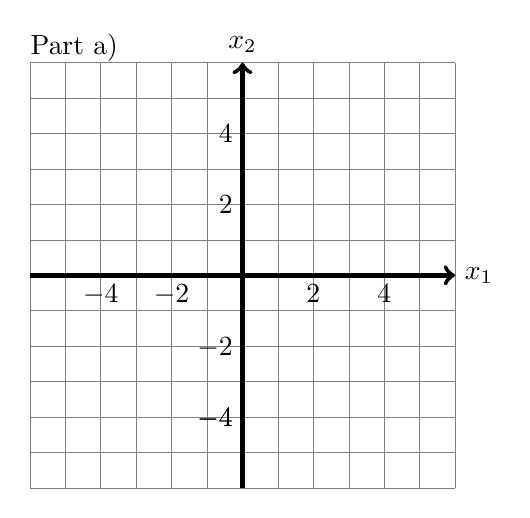
\begin{tikzpicture}[scale=.45]
        \draw[help lines, very thin, gray] (-6, -6) grid (6,6);
        \draw[ultra thick, ->] (-6, 0) -- (6, 0);
        \draw[ultra thick, ->] (0, -6) -- (0, 6);
        \node[overlay, above] at (-4.75, 5.75) { Part a)};
        \node[above] at (0, 6) {$x_2$};
        \node[right] at (6, 0) {$x_1$};
        \node[left] at (0, 2) {$2$};
        \node[below] at (2, 0) {$2$};
        \node[below] at (-2, 0) {$-2$};
        \node[left] at (0, -2.05) {$-2$};  
        \node[left] at (0, 4) {$4$};
        \node[below] at (4, 0) {$4$};
        \node[below] at (-4, 0) {$-4$};
        \node[left] at (0, -4.05) {$-4$};          
        \node[left] at (0, -4.05) {$-4$};          
        \end{tikzpicture}\qquad
        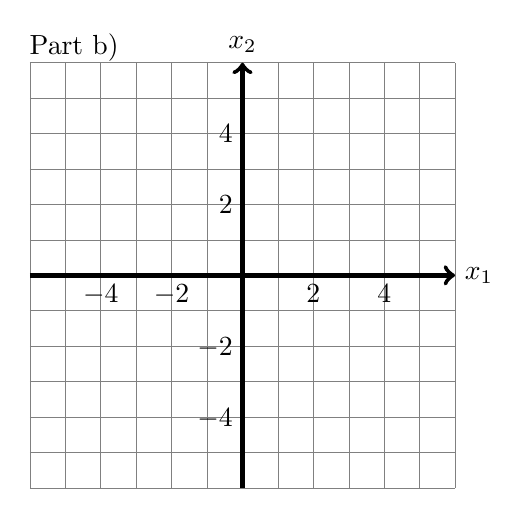
\begin{tikzpicture}[scale=.45]
        \draw[help lines, very thin, gray] (-6, -6) grid (6,6);
        \draw[ultra thick, ->] (-6, 0) -- (6, 0);
        \draw[ultra thick, ->] (0, -6) -- (0, 6);
        \node[overlay, above] at (-4.75, 5.75) { Part b) };
        \node[above] at (0, 6) {$x_2$};
        \node[right] at (6, 0) {$x_1$};
        \node[left] at (0, 2) {$2$};
        \node[below] at (2, 0) {$2$};
        \node[below] at (-2, 0) {$-2$};
        \node[left] at (0, -2.05) {$-2$};  
        \node[left] at (0, 4) {$4$};
        \node[below] at (4, 0) {$4$};
        \node[below] at (-4, 0) {$-4$};
        \node[left] at (0, -4.05) {$-4$};          
        \end{tikzpicture}
        \end{center}
        
        \vspace{24pt}
    \fi
    
    \ifnum \Solutions=1 {\color{DarkBlue} \textit{Solutions.} 
    \begin{enumerate}
        \item[a)] For eigenvalue $\lambda_1$: 
        \begin{align}
            A - \lambda_1 I = \begin{pmatrix} 4&2\\2&7 \end{pmatrix} - 4I = \begin{pmatrix} -4&2\\2&-1 \end{pmatrix}
        \end{align}
        A vector in the null space of this matrix is $v_1 = \begin{pmatrix} 1\\2\end{pmatrix}$. Any nonzero scalar multiple of this vector is also sufficient. For eigenvalue $\lambda_2$: 
        \begin{align}
            A - \lambda_2 I = \begin{pmatrix} 4&2\\2&7 \end{pmatrix}  + I = \begin{pmatrix} 1&2\\2&4 \end{pmatrix}
        \end{align}
        A vector in the null space of this matrix is $v_2 = \begin{pmatrix} -2\\1\end{pmatrix}$. Any nonzero scalar multiple of this vector is also sufficient. Sketching the spans of these vectors gives us the eigenspaces. Be sure to extend the lines to the edges of the graph, because eigenspaces are subspaces. 

        \begin{center}
        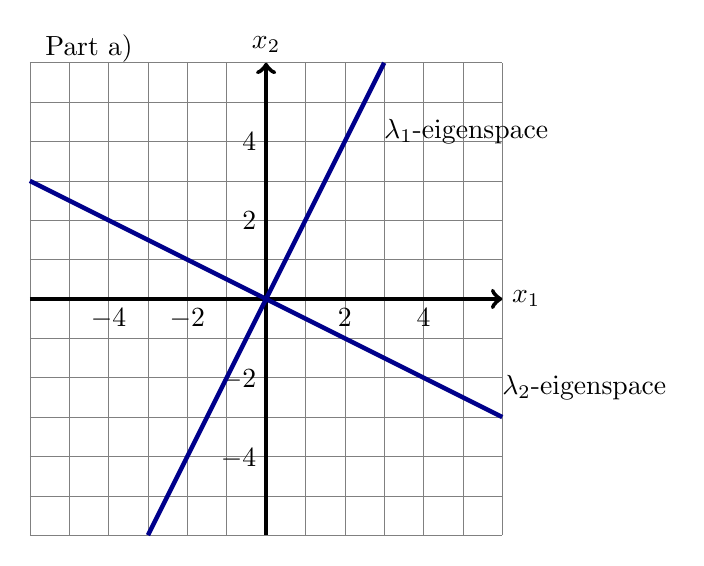
\begin{tikzpicture}[scale=.5]
        \draw[help lines, very thin, gray] (-6, -6) grid (6,6);
        \draw[ultra thick, ->] (-6, 0) -- (6, 0);
        \draw[ultra thick, ->] (0, -6) -- (0, 6);
        \node[overlay, above] at (-4.5, 5.75) {Part a)};
        \node[above] at (0, 6) {$x_2$};
        \node[right] at (6, 0) {$x_1$};
        \node[left] at (0, 2) {$2$};
        \node[below] at (2, 0) {$2$};
        \node[below] at (-2, 0) {$-2$};
        \node[left] at (0, -2.05) {$-2$};  
        \node[left] at (0, 4) {$4$};
        \node[below] at (4, 0) {$4$};
        \node[below] at (-4, 0) {$-4$};
        \node[left] at (0, -4.05) {$-4$};          
        \node[right] at (2.75,4.25) {$\lambda_1$-eigenspace};          
        \draw[ultra thick, DarkBlue,-] (-3, -6) -- (3, 6);
        \node[right] at (5.75,-2.25) {$\lambda_2$-eigenspace};          
        \draw[ultra thick, DarkBlue,-] (-6,3) -- (6,-3);        
        \end{tikzpicture}
        \end{center}
        For this particular matrix, the eigenspaces happen to be perpendicular to each other. Later in the course we will see why this is the case for this matrix. 

        \item[b)] We can approach this in a few different ways. One approach is to work out $p$ using the values of $v_1$ and $v_2$ from the previous part and then compute $Ap$: 
        \begin{align}
            Ap = A (\frac12 v_1 + 2v_2) = \begin{pmatrix} 0&2\\2&3\end{pmatrix}\left( \frac12 \begin{pmatrix} 1\\2 \end{pmatrix} +2 \begin{pmatrix} -2\\1\end{pmatrix}\right) = \begin{pmatrix} 0&2\\2&3\end{pmatrix}\begin{pmatrix} -7/2\\ 3\end{pmatrix} = \begin{pmatrix} 6\\2\end{pmatrix}
        \end{align}
        
        Or, using $Av = \lambda v$ we have that 
        \begin{align}
            Ap = A(\frac12 v_1 + 2v_2) 
            = \frac12 Av_1  + 2Av_2 
            = \frac 12 \lambda_1v_1 + 2\lambda_2v_2 
            = 2\begin{pmatrix} 1\\2 \end{pmatrix} - 2\begin{pmatrix} -2\\1 \end{pmatrix} 
            = \begin{pmatrix} 6\\2\end{pmatrix}
        \end{align}
        The vector $Ap = \begin{pmatrix} 6\\2\end{pmatrix}$ is sketched below. 
            \begin{center}
            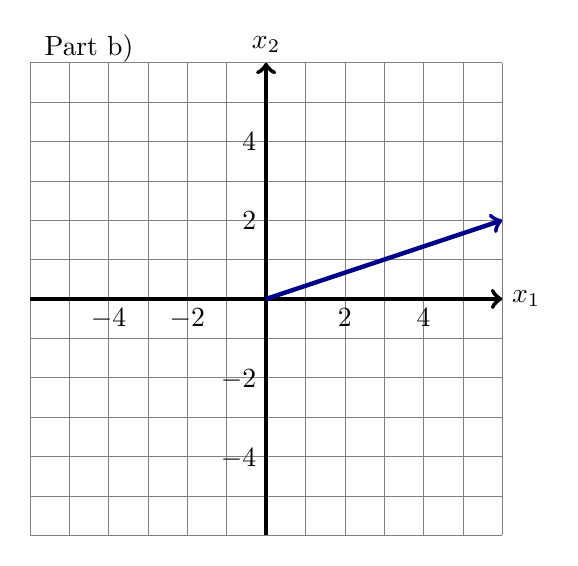
\begin{tikzpicture}[scale=.5]
            \draw[help lines, very thin, gray] (-6, -6) grid (6,6);
            \draw[ultra thick, ->] (-6, 0) -- (6, 0);
            \draw[ultra thick, ->] (0, -6) -- (0, 6);
            \node[overlay, above] at (-4.5, 5.75) {Part b)};
            \node[above] at (0, 6) {$x_2$};
            \node[right] at (6, 0) {$x_1$};
            \node[left] at (0, 2) {$2$};
            \node[below] at (2, 0) {$2$};
            \node[below] at (-2, 0) {$-2$};
            \node[left] at (0, -2.05) {$-2$};  
            \node[left] at (0, 4) {$4$};
            \node[below] at (4, 0) {$4$};
            \node[below] at (-4, 0) {$-4$};
            \node[left] at (0, -4.05) {$-4$};          
            \draw[ultra thick, DarkBlue,->] (0,0) -- (6,2);     
            \end{tikzpicture}
            \end{center}
    \end{enumerate}        
    } 

   \else
      
   \fi
\fi 



\ifnum \Version=2
    \ifnum \Solutions=1 \newpage \fi 
    
    \question[2] The $2\times 2$ matrix $A$ has eigenvalues $\lambda_1=-1$ and $\lambda_2=2$, with eigenspaces indicated in the picture. Vectors $x$ and $y$ are also shown below. Draw $A x$ and $A y$.

    \begin{center}
    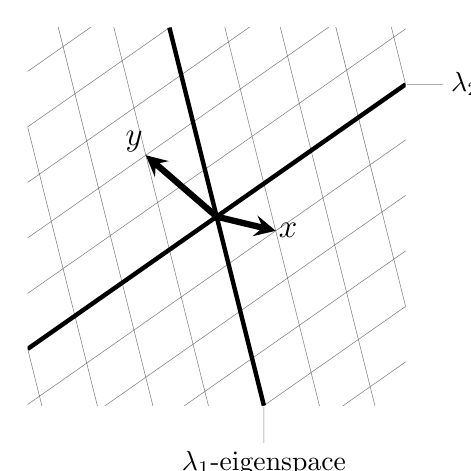
\begin{tikzpicture}[scale=.6,vectorB/.style={-stealth, black, thick, line width=0.8mm}]

      \begin{scope}
      \clip (-4, -4) rectangle (4, 4);
      \begin{scope}[cm={1,2.8/4,1/4,-1,(0,0)}]
        \draw[help lines] (-6, -6) grid (6, 6);
        \draw[vectorB] (0, 0) -- (1, 1) node[right, inner sep=0] {\large $ x$};
        \draw[vectorB] (0, 0) -- (-1, -2) node[above left, inner sep=0] {\large $ y$};
      \end{scope}
      \draw[ultra thick] (-4, -2.8) -- (4, 2.8);
      \draw[ultra thick] (-1, 4) -- (1, -4);
      \node[circle, inner sep=.4mm, fill] at (0, 0) {};
      \end{scope}
      \node[pin={[overlay, inner sep=1mm]0:{$\lambda_2$-eigenspace}}, outer sep=0, inner sep=0] at (4, 2.8) {};
      \node[pin={[overlay, inner sep=1mm]270:{$\lambda_1$-eigenspace}}, outer sep=0, inner sep=0] at (1, -4) {};
    \end{tikzpicture}
    \end{center}    
    
    \ifnum \Solutions=0
        \vspace{12pt}
    \fi

    \ifnum \Solutions=1
        {\color{DarkBlue} 
            \textbf{Solutions}\\
            Take $v_1$ to be any non-zero vector in the $\lambda_1$ eigenspace, and $v_2$ to be any non-zero vector in the $\lambda_2$-eigenspace. We could for example make the following choices for $v_1$ and $v_2$. }
            \begin{center}
            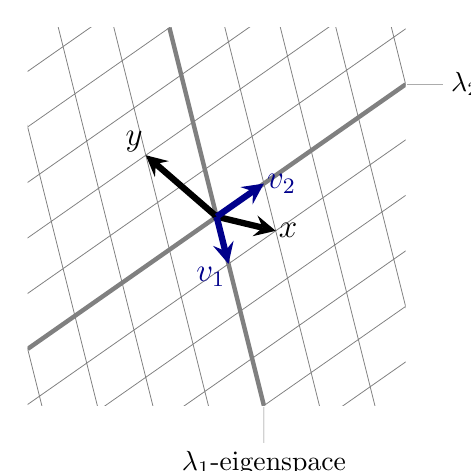
\begin{tikzpicture}[scale=.6,vectorB/.style={-stealth, black, thick, line width=0.8mm},vectorR/.style={-stealth, DarkBlue, thick, line width=0.8mm}]
                \begin{scope}
                    \clip (-4, -4) rectangle (4, 4);
                    \draw[gray,ultra thick] (-4, -2.8) -- (4, 2.8);
                    \draw[gray, ultra thick] (-1, 4) -- (1, -4);
                    \node[circle, inner sep=.4mm, fill] at (0, 0) {};              
                    \begin{scope}[cm={1,2.8/4,1/4,-1,(0,0)}]
                        \draw[help lines,line width=0.1mm] (-6, -6) grid (6, 6);
                        \draw[vectorB] (0, 0) -- (1, 1) node[right, inner sep=0] {\large $ x$};
                        \draw[vectorB] (0, 0) -- (-1, -2) node[above left, inner sep=0] {\large $ y$};
                        \draw[vectorR] (0, 0) -- (0,1) node[below left, inner sep=0] {\large $ v_1$};
                        \draw[vectorR] (0, 0) -- (1, 0) node[right, inner sep=0] {\large $ v_2$};
                    \end{scope}
                \end{scope}
                \node[pin={[overlay, inner sep=1mm]0:{$\lambda_2$-eigenspace}}, outer sep=0, inner sep=0] at (4, 2.8) {};
                \node[pin={[overlay, inner sep=1mm]270:{$\lambda_1$-eigenspace}}, outer sep=0, inner sep=0] at (1, -4) {};
            \end{tikzpicture}
            \end{center}    
            {\color{DarkBlue} 
            With this choice we have $x = v_1 + v_2$, and $y = -2v_1 - v_2$. We want to sketch $A\vec x$ and $A\vec y$, but:
            \begin{align}
                A x &= A(v_1 + v_2) = Av_1 + A v_2 = \lambda_1v_1 + \lambda_2v_2 = -v_1 + 2v_2 \\
                A y &= A(-2v_1 - v_2) = -2Av_1 - A v_2 = -2\lambda_1v_1 - \lambda_2v_2 = 2v_1 - 2v_2 
            \end{align}
            So we need to sketch $Ax = -v_1 + 2v_2$ and $Ay = 2v_1 - 2 v_2$. They are sketched below.}
            \begin{center}
            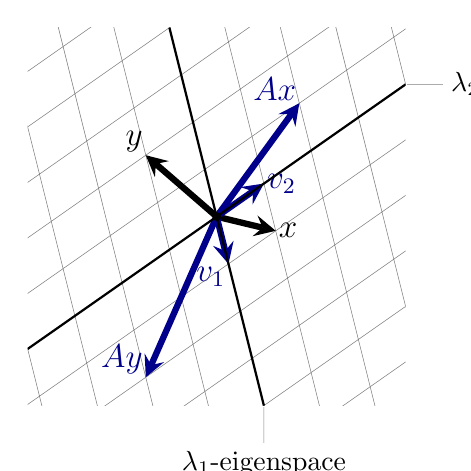
\begin{tikzpicture}[scale=.6,vectorB/.style={-stealth, black, thick, line width=0.8mm},vectorR/.style={-stealth, DarkBlue, thick, line width=0.8mm}]
              \begin{scope}
              \clip (-4, -4) rectangle (4, 4);
              \begin{scope}[cm={1,2.8/4,1/4,-1,(0,0)}]
                \draw[help lines] (-6, -6) grid (6, 6);
                \draw[vectorB] (0, 0) -- (1, 1) node[right, inner sep=0] {\large $ x$};
                \draw[vectorB] (0, 0) -- (-1, -2) node[above left, inner sep=0] {\large $ y$};
                \draw[vectorR] (0, 0) -- (0,1) node[below left, inner sep=0] {\large $ v_1$};
                \draw[vectorR] (0, 0) -- (1, 0) node[right, inner sep=0] {\large $ v_2$};                
                \draw[vectorR] (0, 0) -- (2,-1) node[above left, inner sep=0] {\large $ Ax$};
                \draw[vectorR] (0, 0) -- (-2,2) node[above left, inner sep=0] {\large $ Ay$};
              \end{scope}
              \draw[ thick] (-4, -2.8) -- (4, 2.8);
              \draw[ thick] (-1, 4) -- (1, -4);
              \node[circle, inner sep=.4mm, fill] at (0, 0) {};
              \end{scope}
              \node[pin={[overlay, inner sep=1mm]0:{$\lambda_2$-eigenspace}}, outer sep=0, inner sep=0] at (4, 2.8) {};
              \node[pin={[overlay, inner sep=1mm]270:{$\lambda_1$-eigenspace}}, outer sep=0, inner sep=0] at (1, -4) {};
            \end{tikzpicture}
            \end{center}

    \fi
\fi




\ifnum \Version=3
    \question[2] Calculate the steady state for the Markov chain shown below. Please show your work.  
        \begin{center}
        \begin{tikzpicture}[->,>=stealth',shorten >=1pt,auto,node distance=3cm,thick]
        \tikzstyle{every state}=[circle,fill=gray!10,draw,thick,,font=\bf, line width=0.4mm]
    
        \node[state] (A) {A};
        \node[state]  (B) [right of=A] {B};
        \path 
            (A) edge    [bend left] node {0.3} (B)
                edge    [loop left] node {0.7} (A)
            (B) edge    [loop right] node {0.4} (B) 
                edge    [bend left] node {0.6} (A);
        \end{tikzpicture} 
        \end{center}    

    \ifnum \Solutions=1 {\color{DarkBlue} \textit{Solutions.} 
    
        \begin{align}
            P-I &= \frac{1}{10} \begin{pmatrix} 7 & 6 \\ 3 & 4\end{pmatrix} - \begin{pmatrix} 1&0\\0&1 \end{pmatrix} = \frac{1}{10}\begin{pmatrix}-3&6\\3&-6 \end{pmatrix} \sim \begin{pmatrix}-1&2\\0&0 \end{pmatrix}
        \end{align}
        The steady-state is: 
        $$ \vec q = \frac{1}{3}\begin{pmatrix}2\\1 \end{pmatrix}$$
        } 
    \fi
\fi

\ifnum \Version=4
    \question[2] Calculate the steady state for the Markov chain shown below. Please show your work.  
        \begin{center}
        \begin{tikzpicture}[->,>=stealth',shorten >=1pt,auto,node distance=3cm,thick]
        \tikzstyle{every state}=[circle,fill=gray!10,draw,thick,,font=\bf, line width=0.4mm]
    
        \node[state] (A) {A};
        \node[state]  (B) [right of=A] {B};
        \path 
            (A) edge    [bend left] node {0.3} (B)
                edge    [loop left] node {0.7} (A)
            (B) edge    [loop right] node {0.8} (B) 
                edge    [bend left] node {0.2} (A);
        \end{tikzpicture} 
        \end{center}    

    \ifnum \Solutions=1 {\color{DarkBlue} \textit{Solutions.} 
    
        \begin{align}
            P-I &= \frac{1}{10} \begin{pmatrix} 7 & 2 \\ 3 & 8\end{pmatrix} - \begin{pmatrix} 1&0\\0&1 \end{pmatrix} = \frac{1}{10}\begin{pmatrix}-3&2\\3&-2 \end{pmatrix} \sim \begin{pmatrix}-3&2\\0&0 \end{pmatrix}
        \end{align}
        The steady-state is: 
        $$ \vec q = \frac{1}{5}\begin{pmatrix}2\\3 \end{pmatrix}$$
        } 
    \else
    \vfill         
    \fi
\fi


\ifnum \Version=5
    \question[2] Calculate the steady state for the Markov chain shown below. Please show your work.  
        \begin{center}
        \begin{tikzpicture}[->,>=stealth',shorten >=1pt,auto,node distance=3cm,thick]
        \tikzstyle{every state}=[circle,fill=gray!10,draw,thick,,font=\bf, line width=0.4mm]
    
        \node[state] (A) {A};
        \node[state]  (B) [right of=A] {B};
        \path 
            (A) edge    [bend left] node {0.3} (B)
                edge    [loop left] node {0.7} (A)
            (B) edge    [loop right] node {0.8} (B) 
                edge    [bend left] node {0.2} (A);
        \end{tikzpicture} 
        \end{center}    

    \ifnum \Solutions=1 {\color{DarkBlue} \textit{Solutions.} 
    
        \begin{align}
            P-I &= \frac{1}{10} \begin{pmatrix} 7 & 2 \\ 3 & 8\end{pmatrix} - \begin{pmatrix} 1&0\\0&1 \end{pmatrix} = \frac{1}{10}\begin{pmatrix}-3&2\\3&-2 \end{pmatrix} \sim \begin{pmatrix}-3&2\\0&0 \end{pmatrix}
        \end{align}
        The steady-state is: 
        $$ \vec q = \frac{1}{5}\begin{pmatrix}2\\3 \end{pmatrix}$$
        } 

    \fi
\fi


\ifnum \Version=6
  \TwoStateMarkov{4}{7}
\fi    

\ifnum \Version=7
    \TwoStateMarkov{7}{3} 
\fi

\ifnum \Version=8
    \TwoStateMarkov{7}{5}
\fi      



\ifnum \Version=12 % NOT NEEDED? 
    \question[2] Calculate the steady state for the Markov chain shown below. Please show your work.  
        \begin{center}
        \begin{tikzpicture}[->,>=stealth',shorten >=1pt,auto,node distance=3cm,thick]
        \tikzstyle{every state}=[circle,fill=gray!10,draw,thick,,font=\bf, line width=0.4mm]
    
        \node[state] (A) {A};
        \node[state]  (B) [right of=A] {B};
        \path 
            (A) edge    [bend left] node {0.3} (B)
                edge    [loop left] node {0.7} (A)
            (B) edge    [loop right] node {0.4} (B) 
                edge    [bend left] node {0.6} (A);
        \end{tikzpicture} 
        \end{center}    

    \ifnum \Solutions=1 {\color{DarkBlue} \textit{Solutions.} 
      Find the probability vector in the kernel of $P_I$. 
        \begin{align}
            P-I &= \frac{1}{10} \begin{pmatrix} 7 & 6 \\ 3 & 4\end{pmatrix} - \begin{pmatrix} 1&0\\0&1 \end{pmatrix} = \frac{1}{10}\begin{pmatrix}-3&6\\3&-6 \end{pmatrix} \sim \begin{pmatrix}-1&2\\0&0 \end{pmatrix}
        \end{align}
        The steady-state is: 
        $$ \vec q = \frac{1}{3}\begin{pmatrix}2\\1 \end{pmatrix}$$
        } 
    \else 
        \vfill
    \fi
\fi



\ifnum \Version=13 % NOT NEEDED? 
    \question[2] Calculate the steady state for the Markov chain shown below. Please show your work.  
        \begin{center}
        \begin{tikzpicture}[->,>=stealth',shorten >=1pt,auto,node distance=3cm,thick]
        \tikzstyle{every state}=[circle,fill=gray!10,draw,thick,,font=\bf, line width=0.4mm]
    
        \node[state] (A) {A};
        \node[state]  (B) [right of=A] {B};
        \path 
            (A) edge    [bend left] node {0.2} (B)
                edge    [loop left] node {0.8} (A)
            (B) edge    [loop right] node {0.4} (B) 
                edge    [bend left] node {0.6} (A);
        \end{tikzpicture} 
        \end{center}    

    \ifnum \Solutions=1 {\color{DarkBlue} \textit{Solutions.} 
    
        The steady state has eigenvalue 1. So it is the probability vector in the null space (i.e. - the kernel) of $P-I$. 
        \begin{align} 
            P-I &= \frac{1}{10} \begin{pmatrix} 8 & 6 \\ 2 & 4\end{pmatrix} - \begin{pmatrix} 1&0\\0&1 \end{pmatrix} = \frac{1}{10}\begin{pmatrix}-2&6\\2&-6 \end{pmatrix} \sim \begin{pmatrix}-1&3\\0&0 \end{pmatrix}
        \end{align}
        The steady-state is: 
        $$ \vec q = \frac{1}{4}\begin{pmatrix}3\\1 \end{pmatrix}$$
        } 
    \fi
\fi
        \question[5] Fill in the blanks. You do not need to show your work. 

\begin{parts} 

% A) EIGENVECTORS
\part 
    \ifnum \Version=0
        If $\lambda$ is an eigenvalue of $A$, and $A - \lambda I = \begin{pmatrix} 3&1\\6&2\end{pmatrix}$, then an eigenvector of $A$ is $v = \begin{pmatrix} 1\\k\end{pmatrix}$, where $k = \framebox{\strut\hspace{1cm}}$. 
        
        \ifnum \Solutions=1 {\color{DarkBlue} \textit{Solution:} $v$ has to be in the null space of $A - \lambda I$, so we need to obtain $k$ so that $$\begin{pmatrix} 3&1\\6&2\end{pmatrix}\begin{pmatrix} 1\\k \end{pmatrix} = \begin{pmatrix}0\\0 \end{pmatrix}$$ The only value of $k$ that will satisfy this equation is $k = -3$. } \fi    
    \fi 
    \ifnum \Version=1
        If $A = \begin{pmatrix} 3&1\\6&2\end{pmatrix}$, then $\lambda_1=5$ is an eigenvalue, and a basis for the $\lambda_1$ eigenspace is $v = \begin{pmatrix} 3\\k\end{pmatrix}$, where $k = \framebox{\strut\hspace{1cm}}$. 
        \ifnum \Solutions=1 {\color{DarkBlue} \textit{Solution:} $k=6$ because a vector in the null space of $A-5I = \begin{pmatrix} -2&1\\6&-3\end{pmatrix}$ is $v = \begin{pmatrix}3\\6 \end{pmatrix}$. The dimension of $A-\lambda_1I$ is one, so one vector is sufficient for a basis.  } \fi    
    \fi 
    \ifnum \Version=2
        If $A = \begin{pmatrix} 4&2\\6&5\end{pmatrix}$, then an eigenvector of $A$ that corresponds to eigenvalue $\lambda=1$ is $v = \begin{pmatrix} 2\\k\end{pmatrix}$, where $k = \framebox{\strut\hspace{1cm}}$.     
        \ifnum \Solutions=1 {\color{DarkBlue} \textit{Solution:} 
        $Av = \begin{pmatrix} 8+2k\\12+5k\end{pmatrix}
        =\begin{pmatrix} 2\\k\end{pmatrix}$. 
        So $k=-3$. }
        %   $\begin{pmatrix} 4&2\\6&5\end{pmatrix} - \lambda I_2 = \begin{pmatrix} 3&2\\6&4\end{pmatrix}$, so $v = \begin{pmatrix} 2\\-3\end{pmatrix}$ is in the null space of $A - \lambda I$, so $k = -3$.} 
        \fi    
    \fi 
    \ifnum \Version=3
        If $A = \begin{pmatrix} 5&2\\6&6\end{pmatrix}$, then an eigenvector of $A$ that corresponds to eigenvalue $\lambda=2$ is $v = \begin{pmatrix} 2\\k\end{pmatrix}$, where $k = \framebox{\strut\hspace{1cm}}$.     
        \ifnum \Solutions=1 {\color{DarkBlue} \textit{Solution:} $A - \lambda I_2 = \begin{pmatrix} 3&2\\6&4\end{pmatrix}$, so $v = \begin{pmatrix} 2\\-3\end{pmatrix}$ is in the null space of $A - \lambda I$, so $k = -3$.} \fi    
    \fi 
    \ifnum \Version=4
        If $v_1 = \begin{pmatrix} 2 & 2+4i\end{pmatrix}^T$ is an eigenvector of $A$ that corresponds to eigenvalue $\lambda_1$, then an eigenvector of $A$ that corresponds to the other eigenvalue $\lambda_2$ is $v_2 = \begin{pmatrix} 1 & k\end{pmatrix}^T$, where $k = \framebox{\strut\hspace{1cm}}$.     
        \ifnum \Solutions=1 {\color{DarkBlue} \textit{Solution:} Eigenvectors come in complex conjugate pairs, so if $v_1 = \begin{pmatrix} 2 & 2+4i\end{pmatrix}^T$ is an eigenvector, then $v_2 = \begin{pmatrix} 2 & 2-4i\end{pmatrix}^T$ is an eigenvector for $\lambda_2$. Any non-zero scalar multiple of an eigenvector is also an eigenvector for the same eigenvalue, so if the first entry of $v_2$ needs to be 1, then we can use $v_2 = \begin{pmatrix} 1 & 2=1-2i\end{pmatrix}^T$. So $k = 1-2i$} \fi     
    \fi 
    \ifnum \Version=5
        If $A = \begin{pmatrix} 6&2\\6&7\end{pmatrix}$, then an eigenvector of $A$ that corresponds to eigenvalue $\lambda=3$ is $v = \begin{pmatrix} 2\\k\end{pmatrix}$, where $k = \framebox{\strut\hspace{1cm}}$.     
        \ifnum \Solutions=1 {\color{DarkBlue} \textit{Solution:} $A - \lambda I_2 = \begin{pmatrix} 3&2\\6&4\end{pmatrix}$, so $v = \begin{pmatrix} 2\\-3\end{pmatrix}$ is in the null space of $A - \lambda I$, so $k = -3$.} \fi    
    \fi 
    \ifnum \Version=6
        If $A = \begin{pmatrix} 6&2\\6&7\end{pmatrix}$, then an eigenvector of $A$ that corresponds to eigenvalue $\lambda=10$ is $v = \begin{pmatrix} 1\\k\end{pmatrix}$, where $k = \framebox{\strut\hspace{1cm}}$.     
        \ifnum \Solutions=1 {\color{DarkBlue} \textit{Solution:} $A - \lambda I_2 = \begin{pmatrix} -4&2\\6&-3\end{pmatrix}$, so $v = \begin{pmatrix} 1\\2\end{pmatrix}$ is in the null space of $A - \lambda I$, so $k = 2$.} \fi
    \fi    
    \ifnum \Version=7
        If $A = \begin{pmatrix} 6&2\\6&7\end{pmatrix}$, then an eigenvector of $A$ that corresponds to eigenvalue $\lambda=10$ is $v = \begin{pmatrix} 2\\k\end{pmatrix}$, where $k = \framebox{\strut\hspace{1cm}}$.     
        \ifnum \Solutions=1 {\color{DarkBlue} \textit{Solution:} $A - \lambda I_2 = \begin{pmatrix} -4&2\\6&-3\end{pmatrix}$, so $v = \begin{pmatrix} 2\\4\end{pmatrix}$ is in the null space of $A - \lambda I$, so $k = 4$.}
        \fi
    \fi    
    \ifnum \Version=8    % The other eigenvalue is 15 for this matrix. 
        If $A = \begin{pmatrix} 3&4\\3&14\end{pmatrix}$, then an eigenvector of $A$ that corresponds to eigenvalue $\lambda=2$ is $v = \begin{pmatrix} 4\\k\end{pmatrix}$, where $k = \framebox{\strut\hspace{1cm}}$.     
        \ifnum \Solutions=1 {\color{DarkBlue} \textit{Solution:} $A - \lambda I_2 = \begin{pmatrix} 1&4\\3&12\end{pmatrix}$, so $v = \begin{pmatrix} 4\\-1\end{pmatrix}$ is in the null space of $A - \lambda I$, so $k = -1$.}
        
        \fi
    \fi      

    \ifnum \Version=9
        If $A = \begin{pmatrix} 6&2\\6&7\end{pmatrix}$, then an eigenvector of $A$ that corresponds to eigenvalue $\lambda=3$ is $v = \begin{pmatrix} 2\\k\end{pmatrix}$, where $k = \framebox{\strut\hspace{1cm}}$.     
        \ifnum \Solutions=1 {\color{DarkBlue} \textit{Solution:} $A - \lambda I_2 = \begin{pmatrix} 3&2\\6&4\end{pmatrix}$, so $v = \begin{pmatrix} 2\\-3\end{pmatrix}$ is in the null space of $A - \lambda I$, so $k = -3$.} \fi     
    \fi 

    
% B DIAGOANLIZABILITY AND/OR MULTIPLICITIES
\part 
    \ifnum \Version=0
        If $k = \framebox{\strut\hspace{1cm}}$ then $A = \begin{pmatrix} k&1\\0&3\end{pmatrix}$ is not diagonalizable. 
        
        \ifnum \Solutions=1 {\color{DarkBlue} \textit{Solution:} $k=3$. This is because any matrix with distinct eigenvalues will be diagonalizable, and the eigenvalues of a trianagular matrix are the entries on the main diagonal, so we need $k = 3$ to force $A$ to have repeated eigenvalues. Note that not all matrices with repeated eigenvalues are not diagonalizable, but in this case the matrix is not diagonalizable for $k=3$ because  we won't be able to form $2$ linearly independent eigenvectors to construct $P$ in the diagonalization $A = PDP^{-1}$. } \fi    
    \fi 

    
    \ifnum \Version=1
        Suppose that a $2\times 2$ matrix $A$ is diagonalizable, and that the eigenvalues of $A$ are $\lambda = 1$ and $\lambda= 1/2$. Then as $N$ tends to infinity, what does $\det(A^N)$ tend to? \framebox{\strut\hspace{1cm}}
        \ifnum \Solutions=1 {\color{DarkBlue} \textit{Solution:} Using properties of determinants:
        \begin{align}
            \det(A^N) &= (\det A)^N \\
            &= (\det (PDP^{-1}))^N \\
            &= (\det P \det D \det P^{-1})^N\\
            &= (\det P  \det P^{-1} \det D)^N\\
            &= (\det (P P^{-1}) \det D)^N\\
            &= (\det (I) \det D)^N\\
            &= (\det D)^N
        \end{align}
        But $D$ is diagonal and its eigenvalues are 1 and 0.5, so $D$ is either 
        \begin{align}
            \begin{pmatrix} 1&0\\0&0.5\end{pmatrix} \quad \text{or} \quad \begin{pmatrix} 0.5&0\\0&1\end{pmatrix}
        \end{align}        
        Either way, $\det D = 1 \cdot \frac{1}{2} = \frac12$. So 
        \begin{align}
            \det(A^N) = (\det D)^N = \frac{1}{2^N}
        \end{align}
        So as $N \to \infty$,  $\det(A^N) \to 0$. 
        } \fi    
    \fi 

    
    \ifnum \Version=2
        Suppose that a $2\times 2$ matrix $A$ is diagonalizable, and that the eigenvalues of $A$ are $\lambda = 2$ and $\lambda= 1$. Then $\det(A^4) =  \framebox{\strut\hspace{1cm}}$. 
        \ifnum \Solutions=1 {\color{DarkBlue} \textit{Solution:} Using properties of determinants:
        \begin{align}
            \det(A^4) &= (\det A)^4 \\
            &= (\det (PDP^{-1}))^4 \\
            &= (\det P \det D \det P^{-1})^4\\
            &= (\det P  \det P^{-1} \det D)^4\\
            &= (\det (P P^{-1}) \det D)^4\\
            &= (\det (I) \det D)^4\\
            &= (\det D)^4
        \end{align}
        But $D$ is diagonal and its eigenvalues are 2 and 1, so $D$ is either 
        \begin{align}
            \begin{pmatrix} 1&0\\0&2\end{pmatrix} \quad \text{or} \quad \begin{pmatrix} 2&0\\0&1\end{pmatrix}
        \end{align}        
        Either way, $\det D = 1 \cdot 2 = 2$. So 
        \begin{align}
            \det(A^4) 
            &= (\det D)^4 = 2^4 = 16
        \end{align}        
        } \fi    
    \fi 
    \ifnum \Version=3
        Suppose $A$ is $4\times4$, has only two distinct eigenvalues $\lambda_1$ and $\lambda_2$ and all eigenvalues of $A$ are real. The algebraic multiplicity of $\lambda_1$ is 1, and the algebraic multiplicity of $\lambda_2$ is 3. If $A$ is diagonalizable, the geometric multiplicity of $\lambda_2 = \framebox{\strut\hspace{1cm}}$. 
        \ifnum \Solutions=1 {\color{DarkBlue} \textit{Solution:} for a matrix to be diagonalizable, the geometric multiplicity of each eigenvalue has to be equal to the corresponding algebraic multiplicity. So if the algebraic multiplicity of $\lambda_2$ is 3, then the geometric multiplicity of $\lambda_2$ is also 3. } \fi     
    \fi 
    \ifnum \Version=4
        Suppose $A$ is $4\times4$, has only two distinct eigenvalues $\lambda_1$ and $\lambda_2$ and all eigenvalues of $A$ are real. The algebraic multiplicity of $\lambda_1$ is 1, and the algebraic multiplicity of $\lambda_2$ is 3. If $A$ is diagonalizable, the geometric multiplicity of $\lambda_2 = \framebox{\strut\hspace{1cm}}$. 
        \ifnum \Solutions=1 {\color{DarkBlue} \textit{Solution:} for a matrix to be diagonalizable, the geometric multiplicity of each eigenvalue has to be equal to the corresponding algebraic multiplicity. So if the algebraic multiplicity of $\lambda_2$ is 3, then the geometric multiplicity of $\lambda_2$ is also 3. } \fi      
    \fi 
    \ifnum \Version=5
        Suppose $A$ is $7\times7$, has only two distinct eigenvalues $\lambda_1$ and $\lambda_2$ and all eigenvalues of $A$ are real. The algebraic multiplicity of $\lambda_1$ is 1, and the algebraic multiplicity of $\lambda_2$ is 6. If $A$ is diagonalizable, the geometric multiplicity of $\lambda_2 = \framebox{\strut\hspace{1cm}}$. 
        \ifnum \Solutions=1 {\color{DarkBlue} \textit{Solution:} for a matrix to be diagonalizable, the geometric multiplicity of each eigenvalue has to be equal to the corresponding algebraic multiplicity. So if the algebraic multiplicity of $\lambda_2$ is 6, then the geometric multiplicity of $\lambda_2$ is also 6. } \fi     
    \fi 
    \ifnum \Version=6
        Suppose $A$ is $6\times6$, has only two distinct eigenvalues $\lambda_1$ and $\lambda_2$ and all eigenvalues of $A$ are real. The algebraic multiplicity of $\lambda_1$ is 1, and the algebraic multiplicity of $\lambda_2$ is 5. If $A$ is diagonalizable, the geometric multiplicity of $\lambda_2 = \framebox{\strut\hspace{1cm}}$. 
        \ifnum \Solutions=1 {\color{DarkBlue} \textit{Solution:} for a matrix to be diagonalizable, the geometric multiplicity of each eigenvalue has to be equal to the corresponding algebraic multiplicity. So if the algebraic multiplicity of $\lambda_2$ is 5, then the geometric multiplicity of $\lambda_2$ is also 5. } \fi
    \fi    
    \ifnum \Version=7
        Suppose $A$ is $8\times8$, has only two distinct eigenvalues $\lambda_1$ and $\lambda_2$ and all eigenvalues of $A$ are real. The geometric multiplicity of $\lambda_1$ is 2, and the algebraic multiplicity of $\lambda_2$ is 6. If $A$ is diagonalizable, the geometric multiplicity of $\lambda_2 = \framebox{\strut\hspace{1cm}}$. 
        \ifnum \Solutions=1 {\color{DarkBlue} \textit{Solution:} for a matrix to be diagonalizable, the geometric multiplicity of each eigenvalue has to be equal to the corresponding algebraic multiplicity. So if the algebraic multiplicity of $\lambda_2$ is 6, then the geometric multiplicity of $\lambda_2$ is also 6. } \fi
    \fi    
    \ifnum \Version=8
        Suppose $A$ is $5\times5$, has only two distinct eigenvalues $\lambda_1$ and $\lambda_2$ and all eigenvalues of $A$ are real. The algebraic multiplicity of $\lambda_1$ is 1, and the algebraic multiplicity of $\lambda_2$ is 4. If $A$ is diagonalizable, the geometric multiplicity of $\lambda_2 = \framebox{\strut\hspace{1cm}}$. 
        \ifnum \Solutions=1 {\color{DarkBlue} \textit{Solution:} for a matrix to be diagonalizable, the geometric multiplicity of each eigenvalue has to be equal to the corresponding algebraic multiplicity. So if the algebraic multiplicity of $\lambda_2$ is 4, then the geometric multiplicity of $\lambda_2$ is also 4. } \fi
    \fi      



% C COMPLEX 1
\part 
    \ifnum \Version=0
        An eigenvalue of $A = \begin{pmatrix} 3&-2\\1&1\end{pmatrix}$ is $\lambda_1 = 2+i$. The corresponding eigenvector is $\vec v_1 = \begin{pmatrix} 2 \\ k \end{pmatrix}$, where $k = \framebox{\strut\hspace{1cm}}$. 
        \ifnum \Solutions=1 {\color{DarkBlue} \textit{Solution:} The answer is $k = 1-i$, which could be found by inspection. But an explanation for how to obtain this answer is below. \\[2pt] 
        
        To determine the eigenvector corresponding to $\lambda_1$ we look for a vector in the null space of $A - \lambda_1I$. $$A-\lambda_1 I = \begin{pmatrix} 3&-2\\1&1\end{pmatrix} - (2+i) \begin{pmatrix} 1&0\\0&1 \end{pmatrix} = \begin{pmatrix} 1-i & -2 \\ \ast & \ast \end{pmatrix} $$
        
        The symbol $\ast$ denotes an value that is not needed. If you are wondering why the second row isn't actually needed: don't forget that $A - \lambda I$ is $2\times 2$ and must be singular. So the second row of $A - \lambda I$ must be a multiple of the first, otherwise each row would be pivotal, which would force $A - \lambda I$ to be invertible, which it isn't. When calculating eigenvectors of $2\times 2$ matrices by hand, you never need both rows. You can use both rows in your calculations but you don't need to. 
        
        Vector $\vec v_1$ has to be in the null space of $A - \lambda_1 I$, so \begin{align}
            (A - \lambda_1 I) \vec v & = \begin{pmatrix} 0\\0 \end{pmatrix} \\
            \begin{pmatrix} 1-i & -2 \\ \ast & \ast \end{pmatrix}\begin{pmatrix} 2 \\ k \end{pmatrix}& = \begin{pmatrix} 0\\0 \end{pmatrix} \\ \text{the first row is: } (1-i)\cdot 2 - 2k &= 0 \\
            \text{solve for } k: \quad k &= 1 - i
        \end{align}
        
     } \fi    
    \fi 
    \ifnum \Version=1
        Suppose $A$ is a real $4\times 4$ matrix that has the eigenvalues $3$, $2$, and $1+2i$. Then $A$ also has an eigenvalue that is equal to $\framebox{\strut\hspace{1cm}}$. 
        \ifnum \Solutions=1 {\color{DarkBlue} \textit{Solution:} complex eigenvalues come in conjugate pairs so the remaining eigenvalue is $1-2i$.  } \fi    
    \fi 
    \ifnum \Version=2
        Suppose $A$ is a real $4\times 4$ matrix that has the eigenvalues $3$, $2$, and $1+4i$. Then $A$ also has an eigenvalue that is equal to $\framebox{\strut\hspace{1cm}}$. 
        \ifnum \Solutions=1 {\color{DarkBlue} \textit{Solution:} complex eigenvalues come in conjugate pairs so the remaining eigenvalue is $1-4i$.  } \fi   
    \fi 
    \ifnum \Version=3
        Suppose $A$ is a $4\times 4$ matrix that has the eigenvalues $3$, $2$, and $1+2i$. Then $A$ also has an eigenvalue that is equal to $\framebox{\strut\hspace{1cm}}$. 
        \ifnum \Solutions=1 {\color{DarkBlue} \textit{Solution:} complex eigenvalues come in conjugate pairs so the remaining eigenvalue is $1-2i$.  } \fi      
    \fi 
    \ifnum \Version=4
        Suppose $A$ is a $4\times 4$ matrix that has the eigenvalues $3$, $2$, and $1+2i$. Then $A$ also has an eigenvalue that is equal to $\framebox{\strut\hspace{1cm}}$. 
        \ifnum \Solutions=1 {\color{DarkBlue} \textit{Solution:} complex eigenvalues come in conjugate pairs so the remaining eigenvalue is $1-2i$.  } \fi  
    \fi 
    \ifnum \Version=5
        Suppose $A$ is a $4\times 4$ matrix that has the eigenvalues $3$, $2$, and $1+2i$. Then $A$ also has an eigenvalue that is equal to $\framebox{\strut\hspace{1cm}}$. 
        \ifnum \Solutions=1 {\color{DarkBlue} \textit{Solution:} complex eigenvalues come in conjugate pairs so the remaining eigenvalue is $1-2i$.  } \fi  
    \fi 
    \ifnum \Version=6
       Suppose $A$ is a $4\times 4$ matrix that has the eigenvalues $3$, $-1$, and $1-6i$. Then $A$ also has an eigenvalue that is equal to $\framebox{\strut\hspace{1cm}}$. 
        \ifnum \Solutions=1 {\color{DarkBlue} \textit{Solution:} complex eigenvalues come in conjugate pairs so the remaining eigenvalue is $1+6i$.  }
        \fi
    \fi    
    \ifnum \Version=7
        Suppose $A$ is a $4\times 4$ matrix that has the eigenvalues $3$, $0$, and $7i$. Then $A$ also has an eigenvalue that is equal to $\framebox{\strut\hspace{1cm}}$. 
        \ifnum \Solutions=1 {\color{DarkBlue} \textit{Solution:} complex eigenvalues come in conjugate pairs so the remaining eigenvalue is $-7i$.  } \fi
    \fi    
    \ifnum \Version=8
        Suppose $A$ is a $4\times 4$ matrix that has the eigenvalues $5$, $0$, and $1-3i$. Then $A$ also has an eigenvalue that is equal to $\framebox{\strut\hspace{1cm}}$. 
        \ifnum \Solutions=1 {\color{DarkBlue} \textit{Solution:} complex eigenvalues come in conjugate pairs so the remaining eigenvalue is $1+3i$.  } \fi
    \fi      


% D GOOGLE OR COMPLEX 2
\part 
    \ifnum \Version=0
        $G$ is the Google Matrix for the set of four web pages that link to each other according to the diagram below. If the damping factor is $p=0.85$, then 
        
            \begin{tikzpicture}
                \begin{scope}[->,>=stealth',shorten >=1pt,auto,node distance=1.75cm,ultra thick, main node/.style={circle,fill=gray!10,draw}]
                \node[main node] (1) {A};
                \node[main node] (2) [right of=1] {B};
                \node[main node] (3) [below of=2] {D};
                \node[main node] (4) [right of=2] {C};
                \path[every node/.style={font=\sffamily\small}]
                (4) edge node[below] {} (3)
                (2) edge node [above] {} (1)
                edge [left] node {}  (3) 
                edge [left] node {}  (4) 
                (3) edge node {} (1)
                edge node[right] {} (2);
                %edge node[right] {} (5)
                %(4) edge node [above] {} (5)
                %(4) edge node [above] {} (5);
                \end{scope}
                \node[left] at (-2, -0.85) {$G = p\begin{pmatrix} &&&&&\\&\ &&&&\\&\ &&&&&\\&\ &&&&&\end{pmatrix} + (1-p)\begin{pmatrix} &&&&&\\&\ &&&&\\&\ &&&&&\\&\ &&&&&\end{pmatrix}.$};
            \end{tikzpicture}  
            
        \ifnum \Solutions=1 {\color{DarkBlue} \textit{Solution:} The Google matrix is $$G = p \begin{pmatrix} 1/4&1/3&0&1/2\\1/4&0&0&1/2\\1/4&1/3&0&0\\1/4&1/3&1&0 \end{pmatrix} + (1-p)\begin{pmatrix}1/4&1/4&1/4&1/4\\1/4&1/4&1/4&1/4\\1/4&1/4&1/4&1/4\\1/4&1/4&1/4&1/4 \end{pmatrix}$$ } \fi    
    \fi 
    
    \ifnum \Version=1
      Suppose $A$ is a $2\times2$ matrix with a complex eigenvalue $\lambda = 2+3i$, and an associated eigenvector $v=\begin{pmatrix} 4+i\\5\end{pmatrix}$. Then $A=PCP^{-1}$, where $P=\begin{pmatrix} p_{11}&p_{12}\\p_{21}&p_{22} \end{pmatrix}$, $C=\begin{pmatrix} c_{11}&c_{12}\\c_{21}&c_{22}\end{pmatrix}$ is a real $2\times 2$ matrix, $p_{11} = \framebox{\strut\hspace{1cm}}$ and $c_{11} = \framebox{\strut\hspace{1cm}}$.
      
        \ifnum \Solutions=1 {\color{DarkBlue} \textit{Solution:} Using the $PCP^{-1}$ decomposition that assumes that $C$ is a rotation dilation matrix and $\lambda_1$ is complex, we have 
        \begin{align}
            A=PCP^{-1}, \quad P = \begin{pmatrix} 4&1\\5&0\end{pmatrix}, \quad C=\begin{pmatrix} 2&3\\-3&2\end{pmatrix}
        \end{align}
        Then $p_{11} = 4$, $c_{11} = 2$. Note the following. 
        \begin{itemize}
            \item The question did specify that $P$ and $C$ had to be real. If we were allowed to make $C$ be a diagonal matrix with complex entries, then a correct answer could be obtained by using a diagonalization, and either of the following would also be acceptable. 
        \begin{align}
            A&=PCP^{-1}, \quad P = \begin{pmatrix} 4+i&4-i\\5&5\end{pmatrix}, \quad C = \begin{pmatrix} 2+3i&0\\0&2-3i \end{pmatrix} \\
            A&=PCP^{-1}, \quad P = \begin{pmatrix} 4-i&4+i\\5&5\end{pmatrix}, \quad C= \begin{pmatrix} 2-3i&0\\0&2+3i \end{pmatrix} 
        \end{align}
        In this special case, it would be ok to use $p_{11} = 4+i$ and $c_{11} = 2+3i$, or $p_{11} = 4-i$ and $c_{11} = 2-3i$. But we were told that $C$ had to be real, so this would be only be correct if we didn't have that constraint. 
            \item Don't forget that the $PDP^{-1}$ factorization does not require that the eigenvalues of $A$ be real. The $A=PDP^{-1}$ factorization will exist for $n\times n$ matrix $A$ when $A$ has $n$ linearly independent eigenvectors, regardless of whether the eigenvectors are real or complex. 
            \item Regardless of what factorization was used, the result should give us the same result for $A$. Computing every entry of $P$, $C$, and $P^{-1}$ and then multiplying them together wasn't required for this question (because it requires a lot of calculations). But if you were to hand this calculation over to a computer you should obtain
            \begin{align}
                A = \begin{pmatrix} 14&-10.2\\15&-10\end{pmatrix}
            \end{align}
        \end{itemize}   } \fi    
    \fi 
    \ifnum \Version=2
      Suppose $A$ is a $2\times2$ matrix with a complex eigenvalue $\lambda = 2+3i$, and an associated eigenvector $v=\begin{pmatrix} 4+i\\5\end{pmatrix}$. Then $A=PCP^{-1}$, where $P=\begin{pmatrix} p_{11}&p_{12}\\p_{21}&p_{22} \end{pmatrix}$, $C=\begin{pmatrix} c_{11}&c_{12}\\c_{21}&c_{22}\end{pmatrix}$ is a rotation dilation matrix, $p_{11} = \framebox{\strut\hspace{1cm}}$ and $c_{11} = \framebox{\strut\hspace{1cm}}$. 
        \ifnum \Solutions=1 {\color{DarkBlue} \textit{Solution:} The first column of $P$ is the real part of the eigenvector $v$. The first column of $C$ is from the eigenvalue $2+3i$. 
        $p_{11} = 4$, $c_{11} = 2$.  } \fi    
    \fi 
    \ifnum \Version=3
      Suppose $A$ is a $2\times2$ matrix with a complex eigenvalue $\lambda = 1+3i$, and an associated eigenvector $v=\begin{pmatrix} 2+i\\5\end{pmatrix}$. Then $A=PCP^{-1}$, where $P=\begin{pmatrix} p_{11}&p_{12}\\p_{21}&p_{22} \end{pmatrix}$, $C=\begin{pmatrix} c_{11}&c_{12}\\c_{21}&c_{22}\end{pmatrix}$ is a rotation dilation matrix, $p_{11} = \framebox{\strut\hspace{1cm}}$ and $c_{11} = \framebox{\strut\hspace{1cm}}$. 
        \ifnum \Solutions=1 {\color{DarkBlue} \textit{Solution:} $p_{11} = 2$, $c_{11} = 1$.  } \fi      
    \fi 
    \ifnum \Version=4
        If $x \in \mathbb R^2$ and $A = \begin{pmatrix} 3&-4\\4&3\end{pmatrix}$, then the transform $x \to Ax$ is the composition of a rotation and a scaling. The angle of the rotation is $\phi = \tan^{-1} \left( \, \framebox{\strut\hspace{1cm}}\, \right)$ and the scale factor is $r = \framebox{\strut\hspace{1cm}}$. Assume that $\phi$ measures angles counter-clockwise from the $x_1$-axis. 
        \ifnum \Solutions=1 {\color{DarkBlue} \textit{Solution:} the angle is $\pi = \tan ^{-1} (4/3)$ and the scale factor is $\sqrt{3^2 + 4^2} = 5$. } \fi    
    \fi 
    \ifnum \Version=5
        If $x \in \mathbb R^2$ and $A = \begin{pmatrix} 3&-4\\4&3\end{pmatrix}$, then the transform $x \to Ax$ is the composition of a rotation and a scaling. The angle of the rotation is $\phi = \tan^{-1} \left( \, \framebox{\strut\hspace{1cm}}\, \right)$ and the scale factor is $r = \framebox{\strut\hspace{1cm}}$. Assume that $\phi$ measures angles counter-clockwise from the $x_1$-axis. 
        \ifnum \Solutions=1 {\color{DarkBlue} \textit{Solution:} the angle is $\pi = \tan ^{-1} (4/3)$ and the scale factor is $\sqrt{3^2 + 4^2} = 5$. } \fi  
    \fi 
    \ifnum \Version=6
        If $x \in \mathbb R^2$ and $A = \begin{pmatrix} 3&-2\\2&3\end{pmatrix}$, then the transform $x \to Ax$ is the composition of a rotation and a scaling. The angle of the rotation is $\phi = \tan^{-1} \left( \, \framebox{\strut\hspace{1cm}}\, \right)$ and the scale factor is $r = \framebox{\strut\hspace{1cm}}$. Assume that $\phi$ measures angles counter-clockwise from the $x_1$-axis. 
        \ifnum \Solutions=1 {\color{DarkBlue} \textit{Solution:} the angle is $\pi = \tan ^{-1} (2/3)$ and the scale factor is $\sqrt{3^2 + 2^2} = \sqrt{13}$. } \fi
    \fi    
    \ifnum \Version=7
        If $x \in \mathbb R^2$ and $A = \begin{pmatrix} 3&2\\-2&3\end{pmatrix}$, then the transform $x \to Ax$ is the composition of a rotation and a scaling. The angle of the rotation is $\phi = \tan^{-1} \left( \, \framebox{\strut\hspace{1cm}}\, \right)$ and the scale factor is $r = \framebox{\strut\hspace{1cm}}$. Assume that $\phi$ measures angles counter-clockwise from the $x_1$-axis. 
        \ifnum \Solutions=1 {\color{DarkBlue} \textit{Solution:} the angle is $\pi = \tan ^{-1} (-2/3)$ and the scale factor is $\sqrt{3^2 + 2^2} = \sqrt{13}$. } \fi
    \fi    
    \ifnum \Version=8
        If $x \in \mathbb R^2$ and $A = \begin{pmatrix} 3&-1\\1&3\end{pmatrix}$, then the transform $x \to Ax$ is the composition of a rotation and a scaling. The angle of the rotation is $\phi = \tan^{-1} \left( \, \framebox{\strut\hspace{1cm}}\, \right)$ and the scale factor is $r = \framebox{\strut\hspace{1cm}}$. Assume that $\phi$ measures angles counter-clockwise from the $x_1$-axis. 
        \ifnum \Solutions=1 {\color{DarkBlue} \textit{Solution:} the angle is $\pi = \tan ^{-1} (1/3)$ and the scale factor is $\sqrt{3^2 + 1^2} = \sqrt{10}$. }
        \fi
    \fi      


% E STOCHASTIC MATRICES PROPERTIES OR DYNAMICAL SYSTEMS
\part 
    \ifnum \Version=0
        The steady-state vector of $P=\dfrac14\begin{pmatrix} 3&2\\1&2\end{pmatrix}$ is $\vec q = \begin{pmatrix} c_1 \\c_2 \end{pmatrix}$, where $c_1 = \framebox{\strut\hspace{1cm}}$, $c_2 = \framebox{\strut\hspace{1cm}}$.
        
        \ifnum \Solutions=1 {\color{DarkBlue} \textit{Solution:} the steady state is a probability vector in the null space of $P-I$, and $$P-I = \begin{pmatrix} -1/4&2/4\\1/4&-2/4 \end{pmatrix} \sim \begin{pmatrix} -1&2\\1&-2\end{pmatrix}$$ Then $\begin{pmatrix} 2\\1\end{pmatrix}$ is in the null space. Dividing by the sum of the entries gives us the steady-state, $\vec q = \frac13 \begin{pmatrix} 2\\1\end{pmatrix}$. So $c_1 = 2/3, \ c_2 = 1/3$. } \fi    
    \fi 
    \ifnum \Version=1
        Matrix $A$ is $2\times 2$ with eigenvalues $\lambda_1 = 1$ and $\lambda_2= 1/2$. The corresponding eigenvectors are $v_1 = \begin{pmatrix} 2\\1\end{pmatrix}$ and $v_2=\begin{pmatrix} 2\\3\end{pmatrix}$. If $ p = 3v_1+2v_2$, $A^kp \to \begin{pmatrix} c_1 \\ c_2 \end{pmatrix}$ as $k\to \infty$, then $c_1 = \framebox{\strut\hspace{1cm}}$ and $c_2 = \framebox{\strut\hspace{1cm}}$. 
        \ifnum \Solutions=1 {\color{DarkBlue} \textit{Solution:} $A^kp = A^k(3v_1 + 2v_2) = 3A^kv_1 + 2A^kv_2 = 3\lambda_1^kv_1 + 2\lambda_2^kv_2$. But $\lambda_1^k =1^k = 1$, and $\lambda_2^k = (1/2)^k\to 0$ as $k\to \infty$. So \begin{align}
            \lim_{k \to \infty} A^kp = 3v_1 + 0v_2 = \begin{pmatrix} 6\\3\end{pmatrix}
        \end{align} So $c_1 = 6$, $c_2 = 3$. } \fi    
    \fi 
    \ifnum \Version=2
        If $A$ is a singular $2\times 2$ matrix that is stochastic, the eigenvalues of $A$ are \framebox{\strut\hspace{1cm}} and \framebox{\strut\hspace{1cm}}. 
        \ifnum \Solutions=1 {\color{DarkBlue} \textit{Solution:} singular matrices have an eigenvalue equal to zero and stochastic matrices have an eigenvalue equal to one. So one of the two blanks should be filled with 1 and the other should be filled with 0. } \fi     
    \fi 
    \ifnum \Version=3
        If $A$ is a singular $2\times 2$ matrix that is stochastic, the eigenvalues of $A$ are \framebox{\strut\hspace{1cm}} and \framebox{\strut\hspace{1cm}}. 
        \ifnum \Solutions=1 {\color{DarkBlue} \textit{Solution:} singular matrices have an eigenvalue equal to zero and stochastic matrices have an eigenvalue equal to one. So one of the two blanks should be filled with 1 and the other should be filled with 0. } \fi  
    \fi 
    \ifnum \Version=4
        If $A$ is a singular $2\times 2$ matrix that is stochastic, the eigenvalues of $A$ are \framebox{\strut\hspace{1cm}} and \framebox{\strut\hspace{1cm}}. 
        \ifnum \Solutions=1 {\color{DarkBlue} \textit{Solution:} singular matrices have an eigenvalue equal to zero and stochastic matrices have an eigenvalue equal to one. So one of the two blanks should be filled with 1 and the other should be filled with 0. } \fi  
    \fi 
    \ifnum \Version=5
        If $A$ is a singular $2\times 2$ matrix that is stochastic, the eigenvalues of $A$ are \framebox{\strut\hspace{1cm}} and \framebox{\strut\hspace{1cm}}. 
        \ifnum \Solutions=1 {\color{DarkBlue} \textit{Solution:} singular matrices have an eigenvalue equal to zero and stochastic matrices have an eigenvalue equal to one. So one of the two blanks should be filled with 1 and the other should be filled with 0. } \fi  
    \fi 
    \ifnum \Version=6
        Matrix $A$ is $2\times 2$. Its eigenvalues are $\lambda_1 = 1$ and $\lambda_2= 1/4$. The corresponding eigenvectors are $v_1 = \begin{pmatrix} 3\\2\end{pmatrix}$ and $v_2=\begin{pmatrix} -2\\3\end{pmatrix}$. If $ p = 2v_1+v_2$, and $A^kp \to \begin{pmatrix} c_1 \\ c_2 \end{pmatrix}$ as $k\to \infty$, then $c_1 = \framebox{\strut\hspace{1cm}}$ and $c_2 = \framebox{\strut\hspace{1cm}}$. 
        
        \ifnum \Solutions=1 {\color{DarkBlue} \textit{Solution:} $A^kp = A^k(2v_1 + v_2) = 2A^kv_1 + A^kv_2 = 2\lambda_1^kv_1 + \lambda_2^kv_2$. But $\lambda_1^k =1^k = 1$, and $\lambda_2^k = (1/2)^k\to 0$ as $k\to \infty$. So \begin{align}
            \lim_{k \to \infty} A^kp = 2v_1 + 0v_2 = 2v_1 = \begin{pmatrix} 6\\4\end{pmatrix}
        \end{align} So $c_1 = 6$, $c_2 = 4c$. } \fi    
    
    \fi    
    \ifnum \Version=7
        The steady-state vector of $P=\dfrac15\begin{pmatrix} 2&1\\3&4\end{pmatrix}$ is $\vec q = \begin{pmatrix} c_1 \\c_2 \end{pmatrix}$, where $c_1 = \framebox{\strut\hspace{1cm}}$, $c_2 = \framebox{\strut\hspace{1cm}}$.
        
        \ifnum \Solutions=1 {\color{DarkBlue} \textit{Solution:} the steady state is a probability vector in the null space of $P-I$, and $$P-I = \dfrac15\begin{pmatrix} -3&1\\3&-1 \end{pmatrix} $$ Then $\begin{pmatrix} 1\\3\end{pmatrix}$ is in the null space. Dividing by the sum of the entries gives us the steady-state, $\vec q = \frac14\begin{pmatrix} 1\\3\end{pmatrix}$. So $c_1 = 1/4, \ c_2 = 3/4$. } \fi
    \fi    
    \ifnum \Version=8
        The steady-state vector of $P=\dfrac15\begin{pmatrix} 2&4\\3&1\end{pmatrix}$ is $\vec q = \begin{pmatrix} c_1 \\c_2 \end{pmatrix}$, where $c_1 = \framebox{\strut\hspace{1cm}}$, $c_2 = \framebox{\strut\hspace{1cm}}$.
        
        \ifnum \Solutions=1 {\color{DarkBlue} \textit{Solution:} the steady state is a probability vector in the null space of $P-I$, and $$P-I = \dfrac15\begin{pmatrix} -3&4\\3&-4 \end{pmatrix} $$ Then $\begin{pmatrix} 4\\3\end{pmatrix}$ is in the null space. Dividing by the sum of the entries gives us the steady-state, $\vec q = \frac17\begin{pmatrix} 4\\3\end{pmatrix}$. So $c_1 = 4/7, \ c_2 = 3/7$. } \fi
    \fi      


    \ifnum \Version=9
        The steady-state vector of $P=\dfrac14\begin{pmatrix} 1&2\\3&2\end{pmatrix}$ is $\vec q = \begin{pmatrix} c_1 \\c_2 \end{pmatrix}$, where $c_1 = \framebox{\strut\hspace{1cm}}$, $c_2 = \framebox{\strut\hspace{1cm}}$.
        
        \ifnum \Solutions=1 {\color{DarkBlue} \textit{Solution:} the steady state is a probability vector in the null space of $P-I$, and $$P-I = \dfrac14\begin{pmatrix} -3&2\\3&-2 \end{pmatrix} \sim \begin{pmatrix} -3&2\\3&-2\end{pmatrix}$$ Then $\begin{pmatrix} 2\\3\end{pmatrix}$ is in the null space. Dividing by the sum of the entries gives us the steady-state, $\vec q = \frac15\begin{pmatrix} 2\\3\end{pmatrix}$. So $c_1 = 2/5, \ c_2 = 3/5$. } \fi
    \fi    

\end{parts}
        \ifnum \Solutions=0 \newpage \fi
        \question[0.25] \ID
        \ifnum \Version=0
    \question[3] $A = \begin{pmatrix}-1&1&-1\\1&-1&1\\1&-1&1 \end{pmatrix}$ has only two distinct eigenvalues, $\lambda_1 = -1$ and $\lambda_2 = 0$.   
    \begin{parts} 
        \part Construct the eigenbasis for eigenvalue $\lambda_1 = -1$. Please show your work.
        \ifnum \Solutions = 0  \vspace{6cm} \fi
        
        \part Construct the eigenbasis for eigenvalue $\lambda_2 = 0$. Please show your work.
        \ifnum \Solutions = 0  \vspace{6cm} \fi
        
        \part If possible, construct real matrices $P$ and $D$ such that $A = PDP^{-1}$, where $D$ is a diagonal matrix. 
    \end{parts}

    \ifnum \Solutions=1 {\color{DarkBlue} \textit{Solutions.} 
    \begin{enumerate}
        \item[a)] $$A - (-1) I = \begin{pmatrix} 0&1&-1\\1&0&1\\1&-1&2\end{pmatrix}\sim\begin{pmatrix} 0&1&-1\\1&0&1\\0&0&0\end{pmatrix}$$ A vector in the null space is $$v_1 = \begin{pmatrix}1\\-1\\-1 \end{pmatrix}$$ 
        \item[b)] $$A - (0) I = \begin{pmatrix} -1&1&-1\\1&-1&1\\1&-1&1\end{pmatrix}\sim\begin{pmatrix} -1&1&-1\\0&0&0\\0&0&0\end{pmatrix}$$ The first row gives us the equation $-x_1+x_2-x_3 =0$, or $x_1 = x_2 - x_3$. Vectors in the null space have the form $$x = \begin{pmatrix}x_1\\x_2\\x_3 \end{pmatrix} = \begin{pmatrix}x_2-x_3\\x_2\\x_3 \end{pmatrix} = x_2\begin{pmatrix} 1\\1\\0\end{pmatrix} + x_3 \begin{pmatrix} 1\\0\\-1\end{pmatrix}$$ 
        Two vectors that form a basis for the eigenspace are $$v_2 = \begin{pmatrix} 1\\1\\0\end{pmatrix}, \quad v_3 = \begin{pmatrix} 1\\0\\-1\end{pmatrix}$$ 
        \item[c)] $$P = \begin{pmatrix} 1&1&1\\-1&1&0\\-1&0&-1\end{pmatrix}, \quad D = \begin{pmatrix} -1&0&0\\0&0&0\\0&0&0\end{pmatrix}$$
    \end{enumerate}
    } 
   \fi
\fi 


\ifnum \Version=1
\question[3] Suppose $A = \begin{pmatrix} 5&-2\\1&3 \end{pmatrix}$. 
    \begin{parts} 
        \part Determine the eigenvalues of $A$. Show your work. 
        \ifnum \Solutions = 0 
            \vspace{4cm}
        \else
            {\color{DarkBlue} 
            $$ 0 = \det(A-\lambda I) = (5-\lambda)(3-\lambda) + 2 = \lambda^2 - 8 \lambda + 17 \ \Rightarrow \ \lambda = \frac82 \pm \frac12\sqrt{64 - 68} = 4 \pm i$$ For clarity we could set: $$\lambda_1 = 4-i, \quad \lambda_2 = 4+i$$
            }
        \fi     
        \part Determine the eigenvectors of $A$. Show your work.
        
        \ifnum \Solutions = 0 
            \vspace{2cm}
        \else
            {\color{DarkBlue} Using the symbol $\ast$ to denote a value that is not needed:
            $$(A-\lambda I) = \begin{pmatrix} 5-\lambda & -2 \\ \ast & \ast\end{pmatrix} \ \Rightarrow \ (5-\lambda)x_1 - 2x_2 = 0$$
            We covered why the second row was not needed in lecture. But as a quick reminder: the matrix $A - \lambda I$ is singular, so there can only be one pivot, so each row must be a multiple of each other (otherwise there would be two pivots and the matrix would not be singular). Then if we set $x_2 = 5 - \lambda$ we have some convenient cancellation that allows us to obtain $x_1$ quickly. 
            \begin{align}
                0 
                &= (5-\lambda)x_1 - 2x_2 \\ 
                &= (5-\lambda)x_1 - 2(5 - \lambda) \\ 
                &= x_1 - 2 \\ 
                x_1 &= 2
            \end{align}
            Then the eigenvectors have the form $\vec v = \begin{pmatrix} 2\\5 - \lambda \end{pmatrix}$. And we found that $\lambda = 4 \pm  i$, so the eigenvectors and their corresponding eigenvalues are as follows.  
            \begin{align}
                \lambda_1 &= 4-i \ \Rightarrow \vec v_1 = \begin{pmatrix} 2\\5 - \lambda_1 \end{pmatrix} = \begin{pmatrix} 2\\1+i \end{pmatrix} \\
                \lambda_2 &= 4+i \ \Rightarrow \vec v_2 = \begin{pmatrix} 2\\5-\lambda_2 \end{pmatrix} = \begin{pmatrix} 2\\1-i\end{pmatrix}
            \end{align}
            
            \textbf{Solution Notes} 
            \begin{itemize}
            \item Complex eigenvalues and eigenvectors come in conjugate pairs. So we should find that $\vec v_1$ is the conjugate of $\vec v_2$. 
            \item As you are working similar problems while preparing for an exam or completing homework, note that WolframAlpha and MATLAB are great tools for checking your work. They can give eigenvalues and eigenvectors very quickly. 
            \begin{itemize}
                \item The WolframAlpha syntax you would use to obtain the eigenvectors and eigenvalues is: \{\{5,-2\},\{1,3\}\}. Entering the matrix by itself returns the eigenvalues and eigenvectors, in addition to other information. 
                \item The MATLAB (or OCTAVE) syntax that you would use to obtain the eigenvectors and eigenvalues is: 
                [V,D] = eig([5 -2;1 3]).
            \end{itemize}
            \item You may find that your eigenvectors look very different from what the solutions present. It could be because your work is correct and your eigenvectors are a multiple of the eigenvectors that are in the solutions, and the multiple is a complex number. You can also check your work by using MATLAB or OCTAVE to compute $A\vec v - \lambda \vec v$ and see if you get the zero vector. For example, the MATLAB synatx for checking whether these calculations are correct could be (performed in one line):
            \begin{center}
                A=[5 -2;1 3], v=[2;1+i], A*v - (4-i)*v
            \end{center}
            \item Those of you going on to take a differential equations course may use these sort of calculations to construct solutions to systems of differential equations that involve complex eigenvalues. The solutions to a system of differential equations can involve calculations with complex eigenvalues. 
            \end{itemize}
            }
        \fi                  
        
    \end{parts}
\fi 


\ifnum \Version=2
    \question[3] $A = \begin{pmatrix}2&1&1\\-1&0&-1\\1&1&2 \end{pmatrix}$ has only two distinct eigenvalues, $\lambda_1 = 1$ and $\lambda_2 = 2$.   
    \begin{parts} 
        \part Construct an eigenbasis for eigenvalue $\lambda_1 = 1$. Please show your work.
        \ifnum \Solutions = 0  \vspace{6cm} \fi
        
        \part Construct an eigenbasis for eigenvalue $\lambda_2 = 2$. Please show your work.
        \ifnum \Solutions = 0  \vspace{6cm} \fi
        
        \part If possible, construct real matrices $P$ and $D$ such that $A = PDP^{-1}$, where $D$ is a diagonal matrix. 
    \end{parts}

    \ifnum \Solutions=1 {\color{DarkBlue} \textit{Solutions.} 
    \begin{enumerate}
        \item[a)] For $\lambda_1 = 1$, 
        $$A - (1) I = \begin{pmatrix} 1&1&1\\-1&-1&-1\\1&1&1\end{pmatrix}\sim\begin{pmatrix} 1&1&1\\0&0&0\\0&0&0\end{pmatrix}$$ Vectors in the null space have the form $$x = \begin{pmatrix}x_1\\x_2\\x_3 \end{pmatrix} = \begin{pmatrix}-x_2-x_3\\x_2\\x_3 \end{pmatrix} = x_2\begin{pmatrix} -1\\1\\0\end{pmatrix} + x_3 \begin{pmatrix} -1\\0\\1\end{pmatrix}$$ 
        \item[b)] For $\lambda_2 = 2$, 
        $$A - (2) I = \begin{pmatrix} 0&1&1\\-1&-2&-1\\1&1&0\end{pmatrix}\sim\begin{pmatrix} 1&1&0\\0&1&1\\0&0&0\end{pmatrix}\sim\begin{pmatrix} 1&0&-1\\0&1&1\\0&0&0\end{pmatrix}$$ Vectors in the null space have the form $$x = \begin{pmatrix}x_1\\x_2\\x_3 \end{pmatrix} = \begin{pmatrix}x_3\\-x_3\\x_3 \end{pmatrix} = x_3 \begin{pmatrix} 1\\-1\\1\end{pmatrix}$$ 
        A vector that is a basis for the eigenspace is $$v_3 = \begin{pmatrix} 1\\-1\\1\end{pmatrix}$$ But any non-zero multiple is also ok. 
        \item[c)] $$P = \begin{pmatrix} -1&-1&1\\1&0&-1\\0&1&1\end{pmatrix}, \quad D = \begin{pmatrix} 1&0&0\\0&1&0\\0&0&2\end{pmatrix}$$
    \end{enumerate}
    } 
   \fi
\fi 


\ifnum \Version=3
    \question[3] $A = \begin{pmatrix}3&1&1\\-1&1&-1\\1&1&3 \end{pmatrix}$ has only two distinct eigenvalues, $\lambda_1 = 2$ and $\lambda_2 = 3$.   
    \begin{parts} 
        \part Construct the eigenbasis for eigenvalue $\lambda_1 = 2$. Please show your work.
        \ifnum \Solutions = 0  \vspace{6cm} \fi
        
        \part Construct the eigenbasis for eigenvalue $\lambda_2 = 3$. Please show your work.
        \ifnum \Solutions = 0  \vspace{6cm} \fi
        
        \part If possible, construct real matrices $P$ and $D$ such that $A = PDP^{-1}$, where $D$ is a diagonal matrix. 
    \end{parts}

    \ifnum \Solutions=1 {\color{DarkBlue} \textit{Solutions.} 
    \begin{enumerate}
        \item[a)] For $\lambda_1 = 2$, 
        $$A - (2) I = \begin{pmatrix} 1&1&1\\-1&-1&-1\\1&1&1\end{pmatrix}\sim\begin{pmatrix} 1&1&1\\0&0&0\\0&0&0\end{pmatrix}$$ Vectors in the null space have the form $$x = \begin{pmatrix}x_1\\x_2\\x_3 \end{pmatrix} = \begin{pmatrix}-x_2-x_3\\x_2\\x_3 \end{pmatrix} = x_2\begin{pmatrix} -1\\1\\0\end{pmatrix} + x_3 \begin{pmatrix} -1\\0\\1\end{pmatrix}$$ 
        \item[b)] For $\lambda_2 = 3$, 
        $$A - (3) I = \begin{pmatrix} 0&1&1\\-1&-2&-1\\1&1&0\end{pmatrix}\sim\begin{pmatrix} 1&1&0\\0&1&1\\0&0&0\end{pmatrix}$$ Vectors in the null space have the form $$x = \begin{pmatrix}x_1\\x_2\\x_3 \end{pmatrix} = \begin{pmatrix}x_3\\-x_3\\x_3 \end{pmatrix} = x_3 \begin{pmatrix} 1\\-1\\1\end{pmatrix}$$ 
        A vector that is a basis for the eigenspace is $$v_3 = \begin{pmatrix} 1\\-1\\1\end{pmatrix}$$ But any non-zero multiple is also ok. 
        \item[c)] $$P = \begin{pmatrix} -1&-1&1\\1&0&-1\\0&1&1\end{pmatrix}, \quad D = \begin{pmatrix} 2&0&0\\0&2&0\\0&0&3\end{pmatrix}$$
    \end{enumerate}
    } 
   \fi
\fi 

\ifnum \Version=4
    \question[3] $A = \begin{pmatrix}3&1&1\\-1&1&-1\\1&1&3 \end{pmatrix}$ has only two distinct eigenvalues, $\lambda_1 = 2$ and $\lambda_2 = 3$.   
    \begin{parts} 
        \part Construct the eigenbasis for eigenvalue $\lambda_1 = 2$. Please show your work.
        \ifnum \Solutions = 0  \vspace{6cm} \fi
        
        \part Construct the eigenbasis for eigenvalue $\lambda_2 = 3$. Please show your work.
        \ifnum \Solutions = 0  \vspace{6cm} \fi
        
        \part If possible, construct real matrices $P$ and $D$ such that $A = PDP^{-1}$, where $D$ is a diagonal matrix. 
    \end{parts}

    \ifnum \Solutions=1 {\color{DarkBlue} \textit{Solutions.} 
    \begin{enumerate}
        \item[a)] For $\lambda_1 = 2$, 
        $$A - (2) I = \begin{pmatrix} 1&1&1\\-1&-1&-1\\1&1&1\end{pmatrix}\sim\begin{pmatrix} 1&1&1\\0&0&0\\0&0&0\end{pmatrix}$$ Vectors in the null space have the form $$x = \begin{pmatrix}x_1\\x_2\\x_3 \end{pmatrix} = \begin{pmatrix}-x_2-x_3\\x_2\\x_3 \end{pmatrix} = x_2\begin{pmatrix} -1\\1\\0\end{pmatrix} + x_3 \begin{pmatrix} -1\\0\\1\end{pmatrix}$$ 
        \item[b)] For $\lambda_2 = 3$, 
        $$A - (3) I = \begin{pmatrix} 0&1&1\\-1&-2&-1\\1&1&0\end{pmatrix}\sim\begin{pmatrix} 1&1&0\\0&1&1\\0&0&0\end{pmatrix}$$ Vectors in the null space have the form $$x = \begin{pmatrix}x_1\\x_2\\x_3 \end{pmatrix} = \begin{pmatrix}x_3\\-x_3\\x_3 \end{pmatrix} = x_3 \begin{pmatrix} 1\\-1\\1\end{pmatrix}$$ 
        A vector that is a basis for the eigenspace is $$v_3 = \begin{pmatrix} 1\\-1\\1\end{pmatrix}$$ But any non-zero multiple is also ok. 
        \item[c)] $$P = \begin{pmatrix} -1&-1&1\\1&0&-1\\0&1&1\end{pmatrix}, \quad D = \begin{pmatrix} 2&0&0\\0&2&0\\0&0&3\end{pmatrix}$$
    \end{enumerate}
    } 
   \fi
\fi 

\ifnum \Version=5
    \question[3] $A = \begin{pmatrix}3&1&1\\-1&1&-1\\1&1&3 \end{pmatrix}$ has only two distinct eigenvalues, $\lambda_1 = 2$ and $\lambda_2 = 3$.   
    \begin{parts} 
        \part Construct the eigenbasis for eigenvalue $\lambda_1 = 2$. Please show your work.
        \ifnum \Solutions = 0  \vspace{6cm} \fi
        
        \part Construct the eigenbasis for eigenvalue $\lambda_2 = 3$. Please show your work.
        \ifnum \Solutions = 0  \vspace{6cm} \fi
        
        \part If possible, construct real matrices $P$ and $D$ such that $A = PDP^{-1}$, where $D$ is a diagonal matrix. 
    \end{parts}

    \ifnum \Solutions=1 {\color{DarkBlue} \textit{Solutions.} 
    \begin{enumerate}
        \item[a)] For $\lambda_1 = 2$, 
        $$A - (2) I = \begin{pmatrix} 1&1&1\\-1&-1&-1\\1&1&1\end{pmatrix}\sim\begin{pmatrix} 1&1&1\\0&0&0\\0&0&0\end{pmatrix}$$ Vectors in the null space have the form $$x = \begin{pmatrix}x_1\\x_2\\x_3 \end{pmatrix} = \begin{pmatrix}-x_2-x_3\\x_2\\x_3 \end{pmatrix} = x_2\begin{pmatrix} -1\\1\\0\end{pmatrix} + x_3 \begin{pmatrix} -1\\0\\1\end{pmatrix}$$ 
        \item[b)] For $\lambda_2 = 3$, 
        $$A - (3) I = \begin{pmatrix} 0&1&1\\-1&-2&-1\\1&1&0\end{pmatrix}\sim\begin{pmatrix} 1&1&0\\0&1&1\\0&0&0\end{pmatrix}$$ Vectors in the null space have the form $$x = \begin{pmatrix}x_1\\x_2\\x_3 \end{pmatrix} = \begin{pmatrix}x_3\\-x_3\\x_3 \end{pmatrix} = x_3 \begin{pmatrix} 1\\-1\\1\end{pmatrix}$$ 
        A vector that is a basis for the eigenspace is $$v_3 = \begin{pmatrix} -1\\-1\\1\end{pmatrix}$$ But any non-zero multiple is also ok. 
        \item[c)] $$P = \begin{pmatrix} -1&-1&1\\1&0&-1\\0&1&1\end{pmatrix}, \quad D = \begin{pmatrix} 2&0&0\\0&2&0\\0&0&3\end{pmatrix}$$
    \end{enumerate}
    } 
   \fi
\fi 

\ifnum \Version=6
 \question[3] 
$A = \begin{pmatrix}-1&1&1\\2&0&2\\1&1&-1 \end{pmatrix}$ has only two distinct eigenvalues, $\lambda_1 = -2$ and $\lambda_2 = 2$.   
    \begin{parts} 
        \part Construct the eigenbasis for eigenvalue $\lambda_1 = -2$. Please show your work.
        \ifnum \Solutions = 0  \vspace{6cm} \fi
        
        \part Construct the eigenbasis for eigenvalue $\lambda_2 = 2$. Please show your work.
        \ifnum \Solutions = 0  \vspace{6cm} \fi
        
        \part If possible, construct real matrices $P$ and $D$ such that $A = PDP^{-1}$, where $D$ is a diagonal matrix. 
    \end{parts}

    \ifnum \Solutions=1 {\color{DarkBlue} \textit{Solutions.} 
    \begin{enumerate}
        \item[a)] For $\lambda_1 = -2$, 
        $$A + 2I = \begin{pmatrix} 1&1&1\\2&2&2\\1&1&1\end{pmatrix}\sim\begin{pmatrix} 1&1&1\\0&0&0\\0&0&0\end{pmatrix}$$ Vectors in the null space have the form $$x = \begin{pmatrix}x_1\\x_2\\x_3 \end{pmatrix} = \begin{pmatrix}-x_2-x_3\\x_2\\x_3 \end{pmatrix} = x_2\begin{pmatrix} -1\\1\\0\end{pmatrix} + x_3 \begin{pmatrix} -1\\0\\1\end{pmatrix}$$ 
        \item[b)] For $\lambda_2 = 2$, 
        \begin{align*}
            A - 2 I 
        &= \begin{pmatrix} -3&1&1\\2&-2&2\\1&1&-3\end{pmatrix}
        \sim\begin{pmatrix} -3&1&1\\1&-1&1\\1&1&-3\end{pmatrix}
        \sim\begin{pmatrix} -3&1&1\\1&-1&1\\0&2&-4\end{pmatrix}
        \sim\begin{pmatrix} -3&0&3\\1&0&-1\\0&1&-2\end{pmatrix} 
        \end{align*}
        We could reduce further if we like. But we can see at this point that vectors in the null space have the form $$x = \begin{pmatrix}x_1\\x_2\\x_3 \end{pmatrix} = \begin{pmatrix}x_3\\2x_3\\x_3 \end{pmatrix} = x_3 \begin{pmatrix} 1\\2\\1\end{pmatrix}$$ 
        A vector that is a basis for the eigenspace is $$v_3 = \begin{pmatrix} 1\\2\\1\end{pmatrix}$$ But any non-zero multiple of this vector would also be ok. 
        \item[c)] $$P = \begin{pmatrix} -1&-1&1\\1&0&2\\0&1&1\end{pmatrix}, \quad D = \begin{pmatrix} -2&0&0\\0&-2&0\\0&0&2\end{pmatrix}$$
    \end{enumerate}
    } \fi
\fi    
\ifnum \Version=7
\ifnum \Solutions=1 \newpage \fi
 \question[3] 
$A = \begin{pmatrix}-3&1&1\\4&0&4\\1&1&-3 \end{pmatrix}$ has only two distinct eigenvalues, $\lambda_1 = -4$ and $\lambda_2 = 2$.   
    \begin{parts} 
        \part Construct the eigenbasis for eigenvalue $\lambda_1 = -4$. Please show your work.
        \ifnum \Solutions = 0  \vspace{6cm} \fi
        
        \part Construct the eigenbasis for eigenvalue $\lambda_2 = 2$. Please show your work.
        \ifnum \Solutions = 0  \vspace{6cm} \fi
        
        \part If possible, construct real matrices $P$ and $D$ such that $A = PDP^{-1}$, where $D$ is a diagonal matrix. 
    \end{parts}

    \ifnum \Solutions=1 {\color{DarkBlue} \textit{Solutions.} 
    \begin{enumerate}
        \item[a)] For $\lambda_1 = -4$, 
        $$A + 2I = \begin{pmatrix} 1&1&1\\4&4&4\\1&1&1\end{pmatrix}\sim\begin{pmatrix} 1&1&1\\0&0&0\\0&0&0\end{pmatrix}$$ Vectors in the null space have the form $$x = \begin{pmatrix}x_1\\x_2\\x_3 \end{pmatrix} = \begin{pmatrix}-x_2-x_3\\x_2\\x_3 \end{pmatrix} = x_2\begin{pmatrix} -1\\1\\0\end{pmatrix} + x_3 \begin{pmatrix} -1\\0\\1\end{pmatrix}$$ 
        \item[b)] For $\lambda_2 = 2$, 
        $$A - 2 I = \begin{pmatrix} -5&1&1\\4&-2&4\\1&1&-5\end{pmatrix}\sim\begin{pmatrix} 0&6&-24\\0&-6&24\\1&1&-5\end{pmatrix}\sim\begin{pmatrix} 0&1&-4\\0&0&0\\1&1&-5\end{pmatrix}\sim\begin{pmatrix} 1&0&-1\\0&1&-4\\0&0&0\end{pmatrix}$$ Vectors in the null space have the form $$x = \begin{pmatrix}x_1\\x_2\\x_3 \end{pmatrix} = \begin{pmatrix} x_3\\ 4 x_3\\ x_3 \end{pmatrix} = x_3 \begin{pmatrix} 1\\ 4\\1
        \end{pmatrix}$$ 
        A vector that is a basis for the eigenspace is $v_3 = \begin{pmatrix} 1&4&1\end{pmatrix}^T$. But any non-zero multiple is also ok. 
        \item[c)] $$P = \begin{pmatrix} -1&-1&1\\1&0&4\\0&1&1\end{pmatrix}, \quad D = \begin{pmatrix} -4&0&0\\0&-4&0\\0&0&2\end{pmatrix}$$
    \end{enumerate}
    } \fi
\fi    
\ifnum \Version=8
   \question[3] 
$A = \begin{pmatrix}3&1&1\\1&3&1\\1&1&3 \end{pmatrix}$ has only two distinct eigenvalues, $\lambda_1 = 2$ and $\lambda_2 = 5$.   
    \begin{parts} 
        \part Construct the eigenbasis for eigenvalue $\lambda_1 = 2$. Please show your work.
        \ifnum \Solutions = 0  \vspace{6cm} \fi
        
        \part Construct the eigenbasis for eigenvalue $\lambda_2 = 5$. Please show your work.
        \ifnum \Solutions = 0  \vspace{6cm} \fi
        
        \part If possible, construct real matrices $P$ and $D$ such that $A = PDP^{-1}$, where $D$ is a diagonal matrix. 
    \end{parts}

    \ifnum \Solutions=1 {\color{DarkBlue} \textit{Solutions.} 
    \begin{enumerate}
        \item[a)] For $\lambda_1 = 2$, 
        $$A - 2I = \begin{pmatrix} 1&1&1\\1&1&1\\1&1&1\end{pmatrix}\sim\begin{pmatrix} 1&1&1\\0&0&0\\0&0&0\end{pmatrix}$$ Vectors in the null space have the form $$x = \begin{pmatrix}x_1\\x_2\\x_3 \end{pmatrix} = \begin{pmatrix}-x_2-x_3\\x_2\\x_3 \end{pmatrix} = x_2\begin{pmatrix} -1\\1\\0\end{pmatrix} + x_3 \begin{pmatrix} -1\\0\\1\end{pmatrix}$$ 
        \item[b)] For $\lambda_2 = 5$, 
        $$A - 5 I = \begin{pmatrix} -2&1&1\\1&-2&1\\1&1&-2\end{pmatrix}\sim\begin{pmatrix} -2&1&1\\0&-3/2&3/2\\0&0&0\end{pmatrix}$$ Vectors in the null space have the form $$x = \begin{pmatrix}x_1\\x_2\\x_3 \end{pmatrix} = \begin{pmatrix} x_1\\ x_1\\x_1 \end{pmatrix} = x_3 \begin{pmatrix} 1\\ 1\\1
        \end{pmatrix}$$ 
        A vector that is a basis for the eigenspace is $$v_3 = \begin{pmatrix} 1\\1\\1\end{pmatrix}$$ But any non-zero multiple is also ok. 
        \item[c)] $$P = \begin{pmatrix} -1&-1&1\\1&0&1\\0&1&1\end{pmatrix}, \quad D = \begin{pmatrix} 2&0&0\\0&2&0\\0&0&5\end{pmatrix}$$
    \end{enumerate}
    } \fi
\fi    



\begin{comment}
311 
464
113 

has eigenvalues 8 2 2 .  
\end{comment}



\ifnum \Version=9
    \question[3] $A = \begin{pmatrix}2&1&1\\-1&0&-1\\1&1&2 \end{pmatrix}$ has only two distinct eigenvalues, $\lambda_1 = 1$ and $\lambda_2 = 2$.   
    \begin{parts} 
        \part Construct the eigenbasis for eigenvalue $\lambda_1 = 1$. Please show your work.
        \ifnum \Solutions = 0  \vspace{6cm} \fi
        
        \part Construct the eigenbasis for eigenvalue $\lambda_2 = 2$. Please show your work.
        \ifnum \Solutions = 0  \vspace{6cm} \fi
        
        \part If possible, construct real matrices $P$ and $D$ such that $A = PDP^{-1}$, where $D$ is a diagonal matrix. 
    \end{parts}

    \ifnum \Solutions=1 {\color{DarkBlue} \textit{Solutions.} 
    \begin{enumerate}
        \item[a)] For $\lambda_1 = 1$, 
        $$A - (1) I = \begin{pmatrix} 1&1&1\\-1&-1&-1\\1&1&1\end{pmatrix}\sim\begin{pmatrix} 1&1&1\\0&0&0\\0&0&0\end{pmatrix}$$ Vectors in the null space have the form $$x = \begin{pmatrix}x_1\\x_2\\x_3 \end{pmatrix} = \begin{pmatrix}-x_2-x_3\\x_2\\x_3 \end{pmatrix} = x_2\begin{pmatrix} -1\\1\\0\end{pmatrix} + x_3 \begin{pmatrix} -1\\0\\1\end{pmatrix}$$ 
        \item[b)] For $\lambda_2 = 2$, 
        $$A - (2) I = \begin{pmatrix} 0&1&1\\-1&-2&-1\\1&1&0\end{pmatrix}\sim\begin{pmatrix} 1&1&0\\0&1&1\\0&0&0\end{pmatrix}\sim\begin{pmatrix} 1&0&-1\\0&1&1\\0&0&0\end{pmatrix}$$ Vectors in the null space have the form $$x = \begin{pmatrix}x_1\\x_2\\x_3 \end{pmatrix} = \begin{pmatrix}x_3\\-x_3\\x_3 \end{pmatrix} = x_3 \begin{pmatrix} 1\\-1\\1\end{pmatrix}$$ 
        A vector that is a basis for the eigenspace is $$v_3 = \begin{pmatrix} 1\\-1\\1\end{pmatrix}$$ But any non-zero multiple of this vector is also ok. 
        \item[c)] $$P = \begin{pmatrix} -1&-1&1\\1&0&-1\\0&1&1\end{pmatrix}, \quad D = \begin{pmatrix} 1&0&0\\0&1&0\\0&0&2\end{pmatrix}$$
    \end{enumerate}
    } 
   \fi
\fi 
    \fi    
    \end{questions}
}
\end{document}